%
\documentclass[12pt]{article}
%\documentclass[12pt]{book}
\bibliographystyle{elsevier}
\usepackage{epsfig}
\usepackage{bm}
\usepackage{fancyhdr}
\input epsf
\usepackage[dvips]{color}
\usepackage{lscape}
\usepackage{longtable}
%
\topmargin -0.3in
\headheight 0.0in
\headsep 0.5in
\textheight 9.4in
\oddsidemargin -.0in
\evensidemargin -.0in
\textwidth 6.6in
\renewcommand{\baselinestretch}{1.4}
%
\def\beqn{\begin{eqnarray}}
\def\eeqn{\end{eqnarray}}
\def\beq{\begin{equation}}
\def\eeq{\end{equation}}
%
\newcommand{\la}{\langle}
\newcommand{\ra}{\rangle}
\newcommand{\zh}{z}
\newcommand{\xbj}{x_{\scriptscriptstyle B}}
%
\newcommand{\Epgb}{$\vec ep~\rightarrow~ep(p,\Delta, N^*)\gamma~$}
\newcommand{\Epgl}{$\vec e\vec p~\rightarrow~ep(p,\Delta, N^*)\gamma~$}
\newcommand{\Epgt}{$ep^T~\rightarrow~ep(p,\Delta, N^*)\gamma~$}
\newcommand{\Thgg}{$\theta_{\gamma^*\gamma}~$}
\newcommand{\Phgg}{$\phi_{\gamma^*\gamma}~$}
\newcommand{\Epg}{$ep~\rightarrow~ep\gamma~$}
\newcommand{\Eppiz}{$ep~\rightarrow~ep\pi^0~$}
\newcommand{\Enpip}{$ep~\rightarrow~en\pi^+~$}
\newcommand{\EppiD}{$ep~\rightarrow~e\pi \Delta~$}
\newcommand{\Epeta}{$ep~\rightarrow~ep\eta~$}
\newcommand{\Epr}{$ep~\rightarrow~ep\rho~$}
\newcommand{\EpX}{$ep\rightarrow epX~$}
\newcommand{\EpKY}{$ep~\rightarrow~eKY~$}
\newcommand{\vEpg}{$\vec ep~\rightarrow~ep\gamma~$}
\newcommand{\xidef}{$\xi=x_B\frac{1+\frac{Delta^2}{2Q^2}}{2-x_B+x_B\frac{Delta^2}{2Q^2}}$}
\def\gevc2{(GeV/c)$^2$}
\newcommand{\EpgX}{$ep~\rightarrow~ep\gamma X~$}
\newcommand{\bfk}{\mbox{\boldmath $k$}}
\newcommand{\bfP}{\mbox{\boldmath $P$}}
\newcommand{\bfp}{\mbox{\boldmath $p$}}
\def\VEC#1{\hbox{\boldmath$#1$\unboldmath}}
\def\Vec#1{{\bf #1}}
\def\slash{/\!\!\!}
\def\one{1 \!\! 1}
\def\D{{\mathrm d}}
\def\E{{\mathrm e}}
\def\I{{\mathrm i}}
\renewcommand{\baselinestretch}{1.4} 
\title{The {\tt CLAS12} Physics Program \\[0.3ex]
Studies of Nucleon Structure}

%\author{.........}

%%%%%%%%%%%%%%%%%%%%%%%%%%%%%%%%%%%%%%%%%%%%%%%%%%%%%%
%

\date{\today}
\begin{document}
\thispagestyle{empty}

\pagenumbering{arabic}    
\maketitle
\vspace{2cm}
    
\thispagestyle{empty}
\pagenumbering{arabic}    

\newpage
\tableofcontents
\newpage

\fancypagestyle{myheading}{%                % Redefining plain style
\fancyhf{} % clear all header and footer fields
\fancyhead[C]{\vspace{0.5cm}\line(1,0){500}\vspace{-1.0cm}}
\fancyhead[l]{\mbox{\bfseries CLAS12 Physics}}
\fancyhead[r]{\mbox{\bfseries Version 1.1  \date{\today}}}
\fancyfoot[C]{\mbox{\bfseries  \thepage }}
\fancyfoot[r]{\mbox{\bfseries Physics}}
\fancyfoot[l]{\vspace{-1cm}\line(1,0){500}}
}
\renewcommand{\headrulewidth}{0pt}
\renewcommand{\footrulewidth}{0pt}
%%%\pagestyle{myheading}


%

\newpage

\fancypagestyle{myheading}{%                % Redefining plain style
\fancyhf{} % clear all header and footer fields
\fancyhead[C]{\vspace{0.5cm}\line(1,0){500}\vspace{-0.5cm}}
\fancyhead[l]{\mbox{\bfseries The CLAS12 Physics Program}}
\fancyhead[r]{\mbox{\bfseries Version 1.1  \date{\today}}}
\fancyfoot[C]{\mbox{\bfseries  \thepage }}
\fancyfoot[r]{\mbox{\bfseries Physics Program}}
\fancyfoot[l]{\vspace{-1cm}\line(1,0){500}}
}
\renewcommand{\headrulewidth}{0pt}
\renewcommand{\footrulewidth}{0pt}
\pagestyle{myheading}
\vspace{5cm}
\chapter{Executive Summary}

In the past five decades many important discoveries have been made  
in electron-proton scattering experiments.  The finite size of the 
proton was measured in Hofstadter's pioneering experiment in which 
electrons of 188~MeV energy were elastically scattered off a hydrogen 
target~\cite{hofstadter}.  It demonstrated conclusively that the proton 
is not a Dirac particle but has a finite size. Hofstadter was awarded 
the Nobel prize in 1961 for this discovery.  The energy of Hofstadter's 
accelerator was not high enough to resolve the internal structure of the 
proton but it laid the groundwork for a vigorous research program of 
inclusive electron scattering.  It took another decade, and the 
construction of the powerful electron accelerator and the large magnetic 
spectrometers at the Stanford Linear Accelerator Center (SLAC), to ``see'' 
deep into the proton's interior.  At energies of 20~GeV, experimental 
groups led by Jerome Friedman, Henry Kendall, and Richard Taylor discovered 
``scaling'', i.e. the independence of deeply inelastic structure functions 
of the proton on the virtuality of the electromagnetic probe
\cite{scaling, scaling2}.  These results could only be interpreted in 
terms of electron scattering off point-like ``partons'' inside the proton. 
They were also a triumph for the quarks postulated earlier by theorists 
Murray Gell-Mann~\cite{gellmann} and George Zweig~\cite{zweig} as the 
fundamental building blocks for hadrons.  Gell-Mann received the Nobel 
prize in 1969. For the experimental discovery of the proton's quark structure 
Friedman, Kendall, and Taylor shared the Nobel prize in 1990.  The small 
but significant deviations from scaling that were observed in the SLAC 
experiments also had significant impact on the development of the theory 
of Quantum Chromodynamics (QCD), and are fully explained by the emission 
of gluons from the struck quarks. 

Deeply Inelastic Scattering (DIS) experiments, where only the scattered 
electron is detected, have been carried out up to the highest energies at 
CERN and at DESY. The longitudinal momentum and spin densities of the
quarks have been mapped out in detail.  We have also learned that the 
quarks are not the only tenants of the proton, but that more than 50\% of 
the momentum of the proton is carried by the glue needed to bind the quarks 
together.  More recently, inclusive polarized electron scattering off 
polarized protons led to the ``spin puzzle'', the finding that the quark 
spin contributes less than 25\% of the total spin of the proton, leaving 
much to be understood about the origin of spin~\cite{filipone}.  DIS 
experiments will continue to play an important role in further unraveling 
the valence quark structure, especially under extreme conditions, e.g. 
when one quark carries nearly the full proton momentum.

%%%%%%%%%%%%%%%%%%%%%%%%%%%%%%%%%%%%%%%%%%%%%%%%%%%%%%%%%%%%%%%%%%%%%%%%%
\begin{figure}[htbp]
\vspace{7.7cm} 
\special{psfile=handbag_GPD.ps hscale=33 vscale=33 hoffset=140 voffset=-15}
\caption{\small{The ``handbag'' diagrams for deeply virtual Compton 
scattering (a), and for deeply virtual meson production (b).  Four GPDs 
describe the ``soft'' proton structure part.  They depend not only on $x$, 
but on two more variables: the momentum imbalance of the quark before and 
after the interaction, $\xi$, and the momentum transfer to the proton, $t$.}}
\label{hand_bag}
\end{figure}
%%%%%%%%%%%%%%%%%%%%%%%%%%%%%%%%%%%%%%%%%%%%%%%%%%%%%%%%%%%%%%%%%%%%%%%%%

A glorious past and present is a good basis but not a guarantee for a 
successful future. So, what is the new physics that we are confident will 
shape the future of nuclear physics with electromagnetic probes for the 
coming decades?  While the major discoveries in electromagnetic physics 
have so far come from electron scattering experiments where only the 
scattered electron is measured in magnetic spectrometers, in particular 
measurement of elastic form factors and longitudinal parton densities, they 
are not sufficient to unravel the full structure and internal dynamics of 
the proton.  Semi-exclusive measurements, in which one hadron is observed 
in addition to the scattered electron, are needed to study its flavor 
structure, and only fully exclusive processes in which all final products 
are reconstructed can unravel the complete internal dynamics of the proton.
The experimental and theoretical tools for such an endeavor are now on the 
horizon: electron machines such as CEBAF at 12~GeV, with its CW beams 
and large acceptance detectors operating at high luminosities, are needed 
for the experimental part of such a program, while the new formalism of 
Generalized Parton Distributions (GPDs) provides the theoretical framework 
for the interpretation of the new experiments
\cite{mueller,Ji97_1,Ji97_2,Radyushkin:1996nd,Radyushkin:1997ki}.  The basis 
for this approach are the ``handbag'' diagrams shown in Fig.~\ref{hand_bag}.
Here the electron knocks a quark out of the proton by exchanging a deeply 
virtual (massive) photon. The quark then emits a high energy photon (a) and 
is put back into the proton. Alternatively, a $q\bar q$ pair (meson) is 
created, and one of the quarks is returned into the proton (b).   At 
sufficiently high energies and high virtuality of the exchanged photon 
(``Bjorken regime'') these processes are controlled by perturbative QCD, and 
the results can be interpreted in terms of ``soft'' correlation functions, the 
GPDs. They describe the full complexity of the proton's structure and 
dynamics.        

%%%%%%%%%%%%%%%%%%%%%%%%%%%%%%%%%%%%%%%%%%%%%%%%%%%%%%%%%%%%%%%%%%%%%%%%%
\begin{figure}[ht]
\vspace{8.5cm} 
\special{psfile=fig02-1.ps hscale=50 vscale=50 hoffset=-60 voffset=-55}
\special{psfile=fig02-2.ps hscale=50 vscale=50 hoffset=85 voffset=-58}
\special{psfile=fig02-3.ps hscale=50 vscale=50 hoffset=230 voffset=-65}
\caption{\small{Representations of the proton properties probed in elastic 
scattering (left), deeply inelastic scattering (center), and deeply 
exclusive scattering processes (right). Elastic scattering measures the 
charge density $\rho (b_{\perp})$ as a function of the impact parameter 
$b_{\perp}$.  DIS measures the longitudinal parton momentum fraction density 
$f(x)$. GPDs measure the full correlation function $f(x,b_{\perp},\xi)$ where 
$\xi$ represents the longitudinal momentum imbalance of the struck quark 
before and after the interaction. The graph shows the correlation function 
at $\xi=0$.}}
\label{fig:figure1}
\end{figure}
%%%%%%%%%%%%%%%%%%%%%%%%%%%%%%%%%%%%%%%%%%%%%%%%%%%%%%%%%%%%%%%%%%%%%%%%%

%%%%%%%%%%%%%%%%%%%%%%%%%%%%%%%%%%%%%%%%%%%%%%%%%%%%%%%%%%%%%%%%%%%%%%%%%
\begin{figure}[ht]
\vspace{11.0cm} 
\special{psfile=mb-dgpd.eps hscale=55 vscale=55 hoffset=70 voffset=-70}
\caption{\small{Simulated proton tomography images for the $d$-quarks, 
showing the strong correlation between the transverse size and the 
longitudinal momentum\cite{burkardt}.  For small quark momentum $x$, the 
proton has a large transverse size, and it becomes very dense at large $x$. 
Left column: unpolarized proton, right column: transversely polarized proton.}}
\label{fig:figure2}
\end{figure}
%%%%%%%%%%%%%%%%%%%%%%%%%%%%%%%%%%%%%%%%%%%%%%%%%%%%%%%%%%%%%%%%%%%%%%%%%

What can these experiments tell us about the proton beyond what previous  
experiments have?  Elastic scattering and deeply inelastic scattering give 
us two orthogonal one-dimensional projections of the proton: The quarks in 
the proton are subject to quantum fluctuations, resulting in variations of 
the proton size at a time scale of $< 10^{-23}$ seconds.  Elastic scattering 
measures the probability of finding a proton with a transverse size 
$b_\perp$ matching the resolution of the probe given by the momentum 
transfer $t$: $b_{\perp} \approx {1/\sqrt{|t|}}~$. The expression relates 
the momentum transfer to the transverse size of the proton probed in the 
interaction. Deeply inelastic scattering probes the longitudinal momentum 
distribution of the quarks, but has no sensitivity to the transverse 
dimension.  These two aspects are illustrated in the first two panels of 
Fig.~\ref{fig:figure1}~\cite{belitsky}.  The information resulting from 
these two types of experiments is disconnected, and does not allow us to 
construct the image of a real 3-dimensional proton.   

Deeply exclusive scattering processes connect both transverse and longitudinal 
information including their correlations as described by GPDs. This is shown 
in the third panel of Fig.~\ref{fig:figure1}. The GPDs now depend on 3 
dimensions ($x,\xi,t)$.  Once the GPDs are measured they allow the 
construction of a 3-dimensional image (two in transverse space and one in 
longitudinal momentum) of the proton in what has been called 
``nucleon-tomography''~\cite{burkardt}.  GPDs will allow the study of the
mass and angular momentum distributions of quarks, and the forces and 
pressure distributions in the proton.  

On very general grounds we expect a correlation between the transverse and 
longitudinal variables that, for example at $\xi=0$, could be of the form
\cite{burkardt}:

\begin{equation}
\label{introeq}
H_f(x,0,t) \approx q_f(x)\exp^{-a|t|(1-x) \ln \frac{1}{x}},
\end{equation}

\noindent
where $q_f (x)$ is the forward parton distribution of flavor $f$ and $a$ is
a scale parameter characterizing the transverse size. While the exact shape 
of this function needs to be determined experimentally, it must qualitatively 
contain the correlation between these parameters. Fig.~\ref{fig:figure2} 
illustrates the physical significance of Eq.(\ref{introeq})~\cite{burkardt}. 
The graphs show the strong correlation between the $t$-dependence (transverse 
size $b_{\perp}$) and the $x$-dependence (longitudinal momentum).  For the 
spin-independent GPD $H(x,\xi,t)$ the left panels show the dramatic change in 
transverse profile as a function of longitudinal momentum $x$, while the 
image remains isotropic.  A spatial anisotropy in the proton is observed for 
the spin-dependent GPD $E(x,\xi,t)$ shown in the right panels.   

Electron scattering is the fundamental tool to determine the structure of 
atoms, nuclei, protons, and hadrons.   This program must remain the flagship 
of an electromagnetic laboratory aimed at making fundamental contributions 
at the frontier of hadronic physics.  This continues to be true for 
measurements of form factors and inclusive processes at high $x$. The new 
physics contained in the GPDs will be the climax of electron scattering and 
revolutionize nucleon structure physics.  With the 12~GeV upgrade, JLab will 
be in the unique position to carry out a major part of the program using its 
powerful electron accelerator and its versatile instrumentation. 
The upgraded {\tt CLAS12} detector will make major contributions in many areas
of hadron physics. In particular, {\tt CLAS12} will have design features that 
are essential for probing the new physics of the GPDs. 



\chapter{GPDs and Quark Distributions in Transverse Space}

\section{Introduction}

The challenge of understanding nucleon electromagnetic structure still 
continues after five decades of experimental scrutiny. From the initial 
measurements of elastic form factors to the accurate determination of 
parton distributions through deep inelastic scattering (DIS), the
experiments have increased in statistical and systematic accuracy.  Only 
recently it was realized that in fact the parton distribution functions
represent special cases of a more general, much more powerful, way to 
characterize the structure of the nucleon, the generalized parton 
distributions (GPDs)~\cite{Ji:1996nm,Ji:1996ek,Radyushkin:1996nd,
Radyushkin:1997ki}.  The GPDs are the Wigner quantum phase space 
distribution of quarks in the nucleon -- functions describing the 
simultaneous distribution of particles with respect to both position and 
momentum in a quantum-mechanical system, representing the closest analogue 
to a classical phase space density allowed by the uncertainty principle. 
In addition to the information about the spatial density (form factors) 
and momentum density (parton distribution), these functions reveal the 
correlation of the spatial and momentum distributions, {\it i.e.} how the 
spatial shape of the nucleon changes when probing quarks and gluons of 
different wavelengths.

The concept of GPDs has led to completely new methods of ``spatial imaging''
of the nucleon, either in the form of two-dimensional tomographic images 
(analogous to CT scans in medical imaging), or in the form of genuine 
three-dimensional images (Wigner distributions).  GPDs also allow us to 
quantify how the orbital motion of quarks in the nucleon contributes to the 
nucleon spin -- a question of crucial importance for our understanding of 
the ``mechanics'' underlying nucleon structure.  The spatial view of the 
nucleon enabled by the GPDs provides us with new ways to test dynamical 
models of nucleon structure. 

The mapping of the nucleon GPDs, and a detailed understanding of the
spatial quark and gluon structure of the nucleon, have been widely 
recognized as the key objectives of nuclear physics of the 
next decade. This requires a comprehensive program, combining results
of measurements of a variety of processes in electron--nucleon 
scattering with structural information obtained from theoretical studies, 
as well as with expected results from future lattice QCD simulations.

GPDs, in basic terms, describe the structure of the nucleon probed in 
reactions in which a high-energy, short-distance probe interacts with a 
{\em single quark} in the nucleon.  Mathematically, this is the 
quantum-mechanical amplitude for ``taking out'' a quark from the wave 
function of a fast-moving nucleon and ``putting it back'' with different 
momentum, thereby imparting a certain momentum transfer to the nucleon.
It depends on the fractions of the nucleon momentum carried by the
quark before and after the process, $x+\xi$ and $x-\xi$ ($\xi$ defines the 
longitudinal momentum transfer to the nucleon), as well as on the transverse 
momentum transfer to the nucleon, $\bm{\Delta}_\perp$.  In the special case 
of zero momentum transfer, $\xi = 0$ and $\bm{\Delta}_\perp = 0$, this 
amplitude reduces to the usual parton density of quarks in the nucleon, 
measured in inclusive deep-inelastic $eN$ scattering.  Similarly, in the 
case of non-zero transverse momentum transfer, $\bm{\Delta}_\perp \neq 0$, 
the integral of the GPD over $x$ reduces to the nucleon form factor at 
invariant momentum transfer $t = -\bm{\Delta}_\perp^2$, measured in elastic 
$eN$ scattering. Thus, the GPDs combine the traditional concepts of parton 
density and elastic form factor within a single structure.  The presence of 
spin -- both of the nucleon and the quark -- as well as quark flavors 
($u$, $d$, $s$) leads to the appearance of various independent spin/flavor 
components of the GPDs.  Together, they provide a comprehensive description 
of the quark structure of the nucleon.

The GPDs, however, contain much more information than the parton densities 
and elastic form factors alone. They describe the correlation of the quark 
longitudinal momenta ($x+\xi, x-\xi$) with the transverse momentum transfer 
to the nucleon ($\bm{\Delta}_\perp$).  This information permits a simple 
interpretation in terms of a spatial distribution of quarks in the nucleon. 
For $\xi=0$, the two-dimensional Fourier transform of the GPD with respect to 
$\bm{\Delta}_\perp$ describes the distribution of quarks with longitudinal 
momentum fraction $x$ over the transverse distance, $\bm{b}$, from the center 
of the nucleon (impact parameter).  The integral of this spatial distribution 
over $\bm{b}$ gives the total parton density at a longitudinal momentum 
fraction $x$.  This 1+2-dimensional ``mixed'' momentum and coordinate 
representation corresponds to a set of ``tomographic images'' of the quark 
distribution in the nucleon at fixed longitudinal momentum, $x$. 

A fully 3--dimensional spatial image of the nucleon is obtained when taking 
the Fourier transform of the GPD also with respect to the longitudinal 
momentum transfer to the nucleon, $\xi$, thus localizing the nucleon also in 
longitudinal space. In this case the GPD turns into the Wigner phase space 
distribution of quarks in the nucleon, describing their simultaneous 
distribution with respect to longitudinal momentum $x$ and the conjugate 
coordinate. A quantum phase space distribution describes the distribution
of particles over both coordinate and momentum (or, more generally,
pairs of conjugate variables) in a quantum mechanical system and
represents the closest analogue to a classical phase space density 
allowed by the uncertainty principle.  Fig.~\ref{fig:wigner} shows the 
spatial shape of the nucleon (contours of equal density) for quarks of 
different longitudinal momentum fraction, $x$, as obtained from a model GPD 
consistent with present parton density and form factor data. One sees 
that the effective shape of the nucleon changes with the quark 
momentum fraction probed in a certain reaction. This new 3D representation 
offers unprecedented possibilities not only for visualizing the nucleon as an 
extended object in space, but also for understanding the space-time evolution 
of scattering processes probing the quark and gluon structure of the nucleon.

%%%%%%%%%%%%%%%%%%%%%%%%%%%%%%%%%%%%%%%%%%%%%%%%%%%%%%%%%%%%%%%%%%%%%%%%
\begin{figure}[t]
\vspace{5.0cm}
\special{psfile=../der/wigner.eps hscale=70 vscale=70 hoffset=40 voffset=0}
\caption{\small{``3D images'' of the nucleon as obtained from a model phase 
space distribution incorporating phenomenological information about GPDs.
Shown are constant-density surfaces of the spatial distribution of $u$-quarks, 
for three values of the momentum fraction $x$.  In the valence quark region 
($x \geq 0.1$) the nucleon has a spherical shape. At large $x$ the size 
shrinks and the shape becomes oblate (disk-like). At small $x$, the quarks 
spread out in the longitudinal direction, and the shape becomes prolate 
(cigar-like).}}
\label{fig:wigner}
\end{figure}
%%%%%%%%%%%%%%%%%%%%%%%%%%%%%%%%%%%%%%%%%%%%%%%%%%%%%%%%%%%%%%%%%%%%%%%%

Further motivation for the study of GPDs comes from the fact that certain 
moments of the GPDs -- integrals over the quark momentum fractions -- are 
related to fundamental static properties of the nucleon that cannot directly 
be accessed experimentally otherwise.  In particular, the second moment of 
the GPDs gives the fraction of the nucleon spin carried by the quarks, 
including their spin and orbital angular momentum. Starting with the 
historic measurements by the EMC collaboration 20 years ago, determining 
how the spin of the nucleon is composed from the spins of the quarks and 
gluons and their orbital motion has been the central goal of polarized 
deep-inelastic scattering experiments.  Measurements of the GPDs would give 
access to the quark orbital angular momentum, thus providing information 
about another crucial piece of the nucleon ``spin puzzle''. 

The momentum transfer, $Q^2$, in $eN$ scattering defines the spatial 
resolution of the probe.  The description of hard exclusive processes in 
terms of GPDs applies to the limit of large $Q^2$, where the reaction is 
dominated by the scattering from a single, quasi-free quark (``leading--twist 
approximation'').  At lower $Q^2$, effects related to the interaction of 
quarks during the hard scattering process, or coherent scattering involving 
more than one quark, become important (``higher--twist effects'').  The 
minimum value of $Q^2$ required for the GPD description to be applicable in 
practice depends on the final state, and can ultimately only be determined 
experimentally.  For DVCS (see Fig.~\ref{fig:handbag}), the experience with 
inclusive DIS and other two-photon processes such as 
$\gamma^* \gamma \to \pi^0$ (measured in $e^+e^-$ annihilation) suggest that 
the leading-twist approximation should be reliable already at $Q^2 \sim$ few 
GeV$^2$.   Thus, DVCS can be used to extract information about GPDs at the 
momentum transfers accessible in fixed-target experiments.  For meson 
production, the experience with the pion form factor at high $Q^2$ and 
available meson electroproduction data suggest that higher-twist effects 
are significant up to momentum transfers of $Q^2 \sim$ 10-20~GeV$^2$. While 
such effects can be reduced by forming ratios of observables, or can be 
accounted for in phenomenological models, it seems likely that the use of 
meson production data for a quantitative extraction of GPDs requires 
measurements at significantly higher momentum transfers than in DVCS.

%%%%%%%%%%%%%%%%%%%%%%%%%%%%%%%%%%%%%%%%%%%%%%%%%%%%%%%%%%%%%%%%%%%%%%%%
\begin{figure}[t]
\vspace{5.0cm}
\special{psfile=../der/handbag.eps hscale=120 vscale=120 hoffset=-160 
voffset=-410}
\caption{\small{Reactions in $eN$ scattering probing the generalized parton 
distributions.  Deeply-virtual Compton scattering and meson production 
probe the GPDs at non-zero longitudinal and transverse momentum transfer, 
$\xi \neq 0, \bm{\Delta}_\perp = 0$. Different mesons ($\rho, \pi, K$) 
select different spin-flavor components of the GPDs.}}
\label{fig:handbag}
\end{figure}
%%%%%%%%%%%%%%%%%%%%%%%%%%%%%%%%%%%%%%%%%%%%%%%%%%%%%%%%%%%%%%%%%%%%%%%%

In the $eN \to eN\gamma$ cross section, the DVCS amplitude interferes 
with the known amplitude of the Bethe-Heitler (BH) process, in which the 
final-state photon is emitted from the electron (see Fig.~\ref{dvcsbh}). 
The total cross section is given by~\cite{Belitsky:2001ns}:

\begin{equation}
\frac{d\sigma^{e p \to e p \gamma}}{dx_B dy d\Delta^2 d\varphi} =
\frac{\alpha^3 x_B y}{16 \pi^2 Q^2 \sqrt{1+\epsilon^2}}
\left | \frac{\mathcal T}{e^3} \right |^2 \, ,
\end{equation}

\vskip 0.3cm

\noindent 
where $\epsilon=2 x_B M/Q$, $y$ is the fraction of the electron energy lost
in the nucleon rest frame and $\varphi$ is the angle between the leptonic
plane $(e,e')$ and the photonic plane ($\gamma^*,\gamma$).

%%%%%%%%%%%%%%%%%%%%%%%%%%%%%%%%%%%%%%%%%%%%%%%%%%%%%%%%%%%%%%%%%%%%%%%%
\begin{figure}[ht]
\centerline{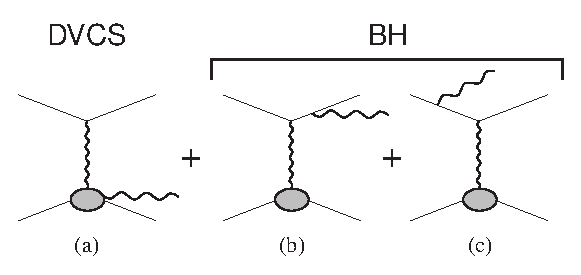
\epsfig{file=../der/diagbh.eps}}
\caption{\small{Diagrams contributing to the electroproduction of a real 
photon. The DVCS process (a) is shown along with the interfering Bethe-Heitler
diagrams (b) and (c).}} 
\label{dvcsbh}
\end{figure}
%%%%%%%%%%%%%%%%%%%%%%%%%%%%%%%%%%%%%%%%%%%%%%%%%%%%%%%%%%%%%%%%%%%%%%%%

The total amplitude $\mathcal T$ is the superposition of the BH and DVCS 
amplitudes:

\begin{eqnarray}
\left | \mathcal T \right |^2 & = & \left | \mathcal T_{BH} \right |^2+\left |
\mathcal T_{DVCS} \right |^2+ \mathcal I \\
\mathcal I & = & \mathcal T_{DVCS}^* \mathcal T_{BH} +
\mathcal T_{DVCS} \mathcal T_{BH}^* \, ,
\end{eqnarray}

\noindent 
where $\mathcal T_{DVCS}$ and $\mathcal T_{BH}$ are the amplitudes for the 
DVCS and Bethe-Heitler processes, and $\mathcal I$ denotes the interference 
between these amplitudes. The individual contributions to the total 
$e p \to e p \gamma$ cross section can be written as (up to twist-3 
contributions)~\cite{Belitsky:2001ns} as:

\begin{eqnarray}
\left| \mathcal T_{BH} \right|^2 & = & \frac{\Gamma_{BH}(x_B,Q^2,t)}{\mathcal P_1(\varphi) P_2(\varphi)}
\left\{ c_0^{BH} + \sum_{n=1}^2 c_n^{BH} \cos (n\varphi) +s_1^{BH} \sin\varphi \right\}  \, , \label{eq:epepgBH} \\
\left| \mathcal T_{DVCS} \right|^2 & = & \Gamma_{DVCS}(x_B,Q^2,t)
\left\{ c_0^{DVCS} + \sum_{n=1}^2 [ c_n^{DVCS} \cos (n\varphi) +s_n^{DVCS} \sin(n\varphi) ] \right\} \, , \label{eq:epepgDVCS} \\
\mathcal I & = & \frac{\Gamma_{I}(x_B,Q^2,t)}{\mathcal P_1(\varphi) P_2(\varphi)} ]
\left\{ c_0^{I} + \sum_{n=1}^3 [ c_n^{I} \cos (n\varphi) +s_n^{I} \sin(n\varphi) ] \right\} \, , \label{eq:epepgI}
\end{eqnarray}

\noindent 
where $\mathcal P_1(\varphi)$ and $\mathcal P_2(\varphi)$ are the BH electron 
propagators and $c_i,s_i$ are azimuthal moments in the corresponding cross 
section contributions.

Depending on whether the beam helicity or target spin is flipped, different 
GPD contributions enter the cross section azimuthal moments ($\sigma_{LU},
\sigma_{UL}$).  In practice, cross section asymmetries are experimentally 
easier to determine:

\begin{equation}
A=\frac{d\sigma^\leftarrow-d\sigma^\rightarrow}{d\sigma^\leftarrow+d\sigma^\rightarrow}\simeq\Gamma_A(x_B,Q^2,t)\frac{s_1^I \sin\varphi + s_2^I \sin 2\varphi}
{c_0^{BH}+c_0^I+\Gamma_Dc_0^{DVCS}+(c_1^{BH}+c_1^I+\Gamma_Dc_0^{DVCS})\cos\varphi} \, ,
\end{equation}

\vskip 0.3cm

\noindent 
where $\Gamma_A,\Gamma_D$ are  known kinematical prefactors. 

DVCS measurements thus allow one to separate the imaginary and real parts of 
the DVCS amplitude (\textit{cf.}\ Fig.~\ref{fig:handbag}) by measuring 
combinations of cross sections and asymmetries with respect to the beam spin 
(helicity), beam charge ($e^+/e^-$), and/or target or recoil polarization. 
The imaginary part of the amplitude probes the GPDs at $x=\xi = \xbj/2$,
the real part probes a certain integral over the quark momentum fractions. 

The different nucleon spin components of the GPDs can be extracted by 
measuring target spin asymmetries. Measurements of the $t$ ($\Delta_\perp$) 
dependence provide the information necessary for transverse nucleon imaging. 
Information about the flavor decomposition requires measurements with both 
protons and neutrons.   Additional information about the spin/flavor 
separation can come from meson production data. Studies of DVCS and meson 
production processes will require a combination of high energy and high beam 
intensity, and are generally much more challenging than traditional inclusive 
scattering experiments.

The {\tt CLAS12} setup will provide unprecedented capabilities for exploring 
nucleon structure in the valence quark region. In particular, it will provide
the  combination of high beam intensity (luminosity), high energy, high beam 
polarization, and advanced detection capabilities to provide a unique 
opportunity for studying nucleon GPDs in exclusive processes in the valence 
region.

\section{Present Experimental Results on Hard Exclusive Processes}

Measurements of exclusive processes at large momentum transfers 
have been carried out in $eN$ scattering experiments with existing 
fixed--target facilities (HERMES at DESY, JLab with 6~GeV beam 
energy) and the HERA collider. These studies have demonstrated the basic 
feasibility of such measurements, and have provided crucial evidence for 
the applicability of a GPD--based description of such processes.
They are also providing the first useful constraints for GPD phenomenology.

Experiments at fixed--target facilities aim to extract the
interference terms between the DVCS and the Bethe--Heitler (BH) amplitudes
in the $eN \to e'N\gamma$ cross section. The interference terms are 
experimentally accessible from combinations of measurements of the
spin--dependent and independent cross sections and relative asymmetries,
as well as from measurements of the beam charge dependence ($e^+ / e^-$)
of the cross section. In kinematic regions where the BH amplitude is much 
larger than the DVCS amplitude, the interference with the BH amplitude acts 
as a natural ``amplifier and filter'' for the DVCS amplitude, boosting
it to comfortably measurable levels. 

%%%%%%%%%%%%%%%%%%%%%%%%%%%%%%%%%%%%%%%%%%%%%%%%%%%%%%%%%%%%%%%%%%%%%%%%
\begin{figure}[ht]
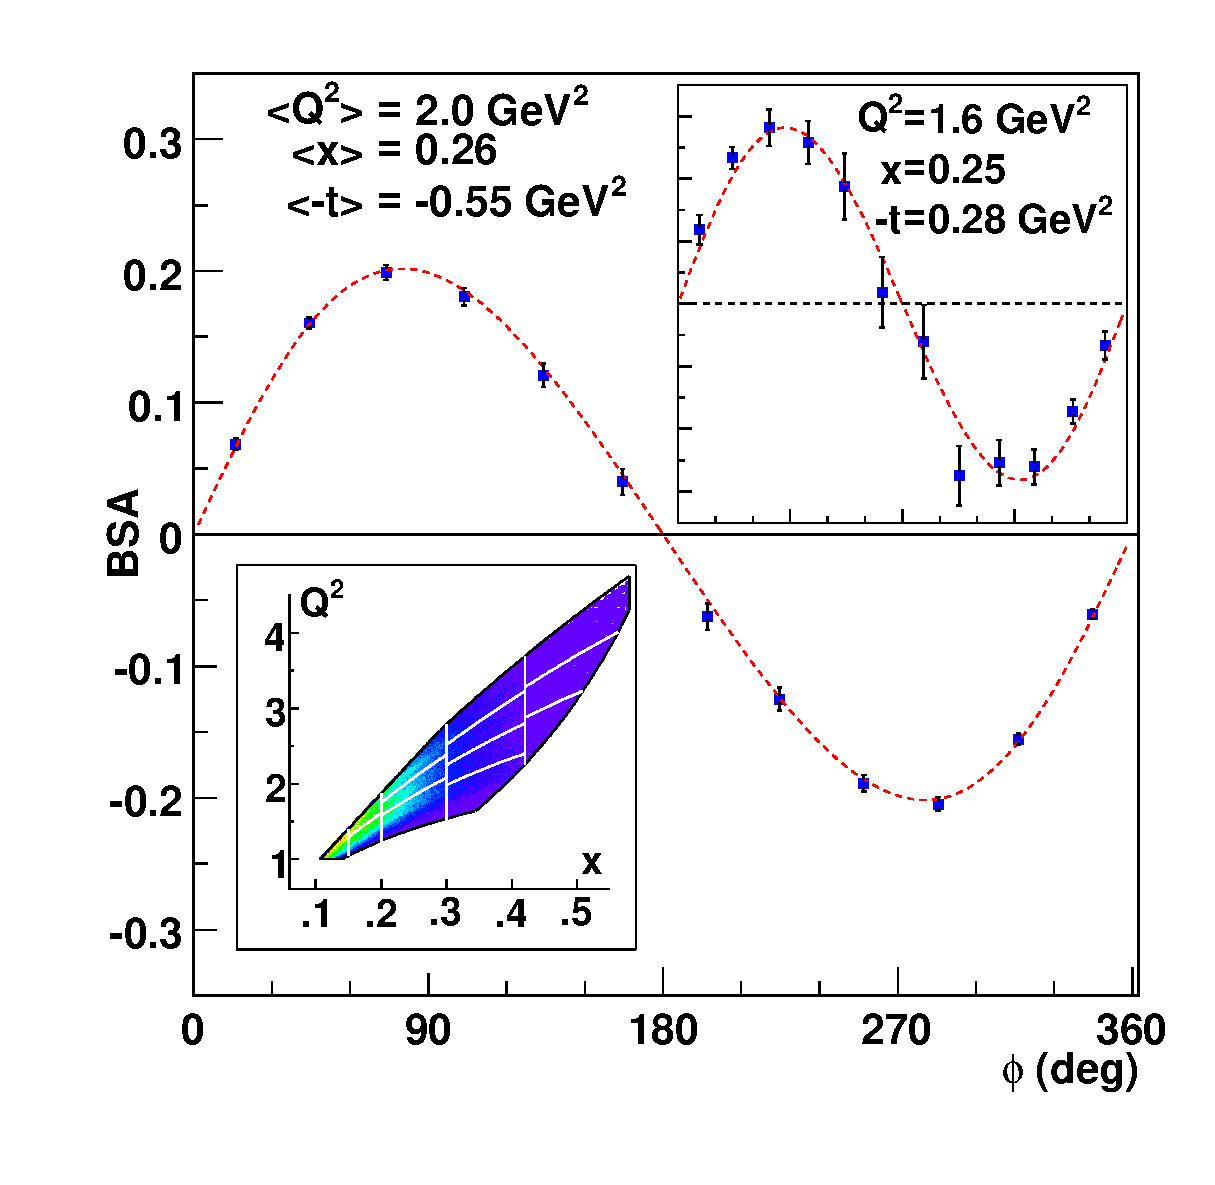
\includegraphics[width=0.99\textwidth]{../der/WP_CLAS_ALU.eps}
\caption{\small{Measurements of the beam spin asymmetry, $A_{LU}$, of the 
$eN \to e'N\gamma$ cross section from {\tt CLAS} at 6~GeV.  The plot in
the lower left corner shows the kinematic coverage in $\xbj$ and $Q^2$.
The main plot shows the beam spin asymmetry vs. $\phi$ integrated over all
kinematics (the average values are shown in the upper left of the plot.  In
the upper right of the plot, the beam spin asymmetry is shown for one of
our many kinematic points as an illustration.  The $\sin \phi$ dependence 
is characteristic of the BH-DVCS interference cross section.  The magnitude 
of the asymmetry can be related to a linear combination of the GPDs 
at $x = \xi$.}}
\label{fig:CLAS_e1}
\end{figure}
%%%%%%%%%%%%%%%%%%%%%%%%%%%%%%%%%%%%%%%%%%%%%%%%%%%%%%%%%%%%%%%%%%%%%%%%

Measurements of the beam spin asymmetry in $eN \to e'N\gamma$ have been 
performed by HERMES ($0.02 < \xbj < 0.3$)~\cite{Airapetian:2001yk}, {\tt CLAS}
\cite{Stepanyan:2001sm,JLabExp:E01-113} and Hall A ($0.15 < \xbj < 0.55$)
\cite{JLabExp:E00-110}.  Fig.~\ref{fig:CLAS_e1} shows the kinematic coverage 
of the {\tt CLAS} detector at 5.7~GeV, as well as the results for the 
asymmetry in a typical $(\xbj, Q^2)$ bin.  A new inner calorimeter was used 
to detect photons at small scattering angles.  The azimuthal angle dependence 
of the asymmetry clearly exhibits the $\sin\phi$ behavior characteristic
of the BH--DVCS interference. This asymmetry can be related to a linear 
combination of GPDs at $x = \xi$; the experimental results are consistent 
with the predictions of present GPD models. An important point is that with 
the {\tt CLAS} detector data in all $(\xbj, Q^2, t)$ bins are taken 
simultaneously, making it possible to extract information about the GPDs 
over a wide kinematic range.

While the unpolarized GPD $\cal H$ dominates the beam spin asymmetry at 
small $t$~\cite{Belitsky:2001ns}, $\sigma_{LU} \sim F_1{\cal H}-\xi F_2{\cal 
\widetilde H}$, the target single spin asymmetry at small $t$ has a 
significant contribution from the polarized GPD $\cal \widetilde H$
\cite{Belitsky:2001ns}: $\sigma_{UL} \sim F_1{\cal \widetilde H}-\xi 
F_2{\cal H}$.  Therefore, a combined analysis of the beam and target single 
spin asymmetries will allow for separation of $\cal H$ and $\cal \widetilde H$.

Recently published results by the {\tt CLAS} collaboration on the first 
measurements of the target spin asymmetry~\cite{Chen:2006na} confirmed again 
that the factorization is likely to be applicable at $Q^2$ values as low as 
2~GeV$^2$. These measurements eventually will allow one to separate the 
contributions from unpolarized and polarized nucleon GPDs.  An order of 
magnitude more data are expected from JLab during the next two years, which 
would allow for more accurate extraction of GPD parameters. 

The measurements of the DVCS cross sections and beam spin asymmetries carried 
out by JLab with 6~GeV beam energy support the theoretical expectation of 
dominance of the single-quark reaction mechanism (leading-twist approximation) 
for DVCS for momentum transfers $Q^2$ of a few GeV$^2$, essential for the GPD 
interpretation of the $eN \to e'N\gamma$ data.  They also demonstrate the 
feasibility of accurate differential measurements of the $t$-dependence of the 
cross sections needed for the GPD-based reconstruction of the spatial images 
of the nucleon.

The HERMES collaboration measured for the first time the beam charge 
asymmetry of the cross section, which probes a dispersive integral of the 
GPDs over the quark momentum fractions \cite{Airapetian:2006zr}.  DVCS 
cross sections at high $Q^2$ were measured at HERA
\cite{Chekanov:2003ya,Adloff:2001cn}, including its $t$-dependence; the 
results are well described by leading-order (LO) and next-to-leading order 
(NLO) QCD calculations incorporating QCD evolution of the GPDs, thus fully 
confirming the applicability of QCD factorization to exclusive processes 
at high energies.

\subsection{GPD Measurements with Jefferson Laboratory at 12 GeV}

{\tt CLAS12} will provide a unique combination of high beam intensity 
(luminosity), high energy, and large--acceptance detectors, which will 
enable studies of exclusive processes such as DVCS and meson production 
in the valence quark region.

%%%%%%%%%%%%%%%%%%%%%%%%%%%%%%%%%%%%%%%%%%%%%%%%%%%%%%%%%%%%%%%%%%%%%%%%
\begin{figure}[ht]
\centerline{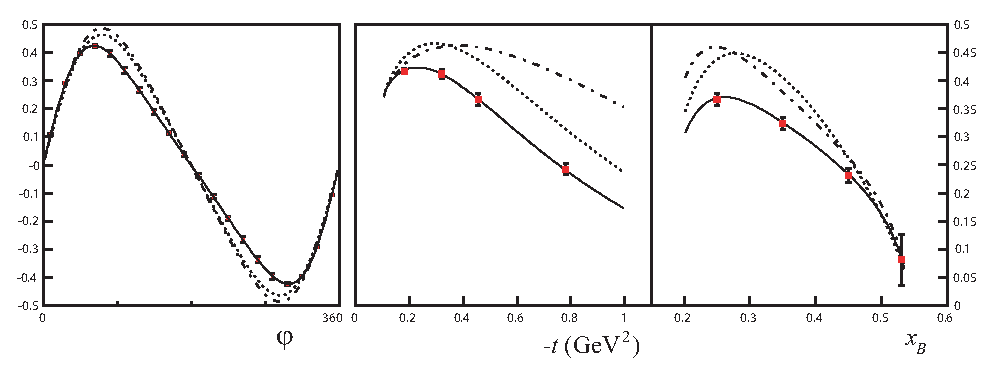
\epsfig{file=../der/asymmetry_detail.eps,width=\linewidth}}
\caption{\small{On all figures: points in red represent data with statistical 
error bars. Lines are models with different input parameters, none of which 
includes twist-3 contributions:  The full line is a model with a Regge-type 
$t$-dependence and D-term. The dotted line includes the Regge-type 
$t$-dependence but has no D-term. The dash-dotted line has the D-term but the 
$t$ dependence only comes from form factors. Left figure: Beam spin asymmetry 
(BSA) as a function of $\varphi$ for $<x_B>=0.2$, $<Q^2>=3.3$~GeV$^2$, and 
$<-t>=0.45$~GeV$^2$. Middle figure: BSA as a function of $-t$ for $<x_B>=0.2$, 
$<Q^2>=3.3$~GeV$^2$, and $\varphi=90^\circ$. Right figure: BSA as a function 
of $x_B$ for $t=0.45$~GeV$^2$, $<Q^2>=3.3$~GeV$^2$ and $\varphi=90^\circ$.}}
\label{fig:asymbig}
\end{figure}
%%%%%%%%%%%%%%%%%%%%%%%%%%%%%%%%%%%%%%%%%%%%%%%%%%%%%%%%%%%%%%%%%%%%%%%%

Detection of the photon in the {\tt CLAS} inner calorimeter, in addition 
to the recoil proton and scattered electron, provides the exclusivity 
condition crucial for complete control over different background processes. 
Using the $epX$ sample  has its own advantages with regard to background 
suppression ($\pi^0$) and azimuthal angle coverage.  The two samples probe 
$ep \to e'\gamma p$ in regions of different relative magnitudes of the DVCS 
and Bethe-Heitler amplitudes.  In this way, GPDs can be extracted using both 
absolute cross section and polarization asymmetry data. The possibility to 
use both methods in experiments at a single facility represents a crucial 
advantage of {\tt CLAS12}.

%%%%%%%%%%%%%%%%%%%%%%%%%%%%%%%%%%%%%%%%%%%%%%%%%%%%%%%%%%%%%%%%%%%%%%%%
\begin{figure}[ht]
\begin{center}
\epsfig{file=../der/tsa_phi_comp.epsi, totalheight=15cm, width=6.5cm, angle=270}
\caption{\small{(a). Target spin asymmetry versus $\varphi$ for 
$Q^2$=4.1~GeV$^2$, $x_B$=0.36, and $-t$=0.52~GeV$^2$. The black points show 
the values from Ref.~\cite{Vanderhaeghen:1999xj} using CTEQ6 PDFs with the 
estimated errors from the proposed measurement. The red solid curve is using 
MRST02 PDFs with $E=\widetilde{E}$=0, and for the blue dashed curve is 
$\widetilde{H}$ is also set to zero. (b). $\sin{\varphi}$ moments of the 
target spin asymmetry versus $-t$ at $Q^2$=4.1~GeV$^2$ and $x_B$=0.36, and 
(c). versus $x_B$ at $Q^2$=4.1~GeV$^2$ and $-t$=0.52~GeV$^2$. The projected 
error bars represent the statistical uncertainties only.}} 
\label{Fig:TsaPhiComp}
\end{center}
\end{figure}
%%%%%%%%%%%%%%%%%%%%%%%%%%%%%%%%%%%%%%%%%%%%%%%%%%%%%%%%%%%%%%%%%%%%%%%%

To separate the different spin components of the GPDs, measurements of a 
variety of polarization observables (beam and target spin) will be performed. 
The longitudinal beam single spin asymmetry, $A_{LU}$ (see 
Fig.~\ref{fig:asymbig}), will access mainly the unpolarized Dirac GPD, 
$\cal H$.  Combined analysis of the DVCS data on a longitudinally polarized 
target single spin asymmetry (see Fig.~\ref{Fig:TsaPhiComp}) with the beam 
single spin asymmetry will provide separation of contributions from 
unpolarized and polarized GPDs.  The double spin asymmetry for longitudinal 
target polarization, $A_{LL}$, provides information on the real part of the 
corresponding GPDs, complementary to beam charge asymmetries.
 
The results of these measurements can directly be translated into transverse 
spatial images of the nucleon. As an example, Fig.~\ref{fig:H_proj} shows 
the projected results for the Dirac GPD, $\cal H$, as a function of $x$ and 
$t$, and its corresponding transverse spatial representation.  Complementary 
information can be obtained about integrals of the GPDs over the quark 
momentum fraction. With the help of GPD parameterizations, this information 
can be used to construct 2-dimensional tomographic images of the nucleon.

%%%%%%%%%%%%%%%%%%%%%%%%%%%%%%%%%%%%%%%%%%%%%%%%%%%%%%%%%%%%%%%%%%%%%%%%
\begin{figure}
\begin{tabular}{cc}
\parbox[c]{0.4\textwidth}{
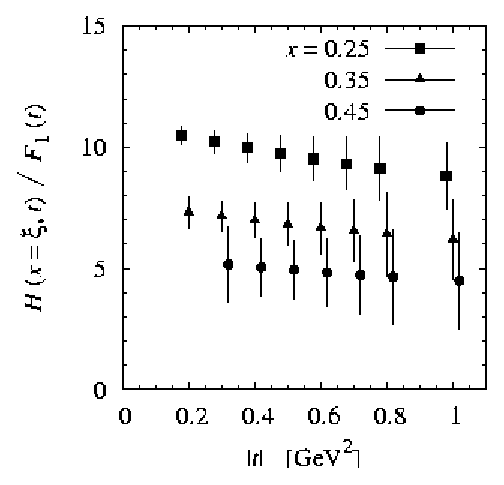
\includegraphics[width=0.4\textwidth]{../der/gpdtdep.eps}}
&
\parbox[c]{0.56\textwidth}{
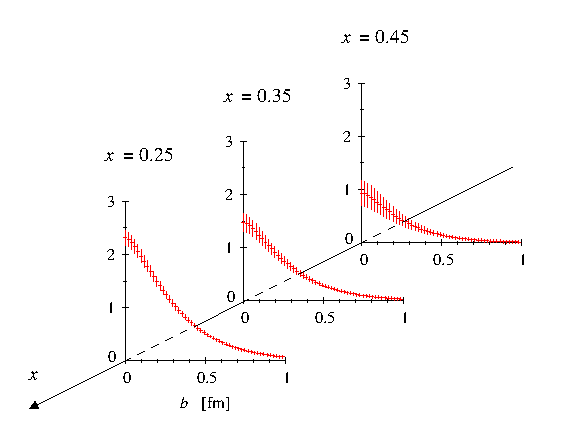
\includegraphics[width=0.56\textwidth]{../der/spatial_narrow.eps}}
\end{tabular}
\caption{\small{Left: Projected results for the Dirac GPD of the proton, 
${\cal H}(x = \xi, t)$, as a function of $x$ and $t$, as extracted from the 
DVCS beam spin asymmetry, $A_{LU}$, measured at JLab at 12~GeV. Shown is the 
ratio of the GPD to the the proton's Dirac form, $F_1(t)$.  Right: Transverse 
spatial image of the proton obtained by Fourier-transforming the measured GPD. 
The errors were estimated assuming a dipole-like $t$-dependence.}}
\label{fig:H_proj}
\end{figure}
%%%%%%%%%%%%%%%%%%%%%%%%%%%%%%%%%%%%%%%%%%%%%%%%%%%%%%%%%%%%%%%%%%%%%%%%

Additional information about the flavor structure of GPDs will come from 
ratios of meson production cross sections in channels with the same 
spin/parity quantum numbers, such as $\eta / \pi^0$ and $K^* / \rho^+$. 
These channels will be measured simultaneously with DVCS, not requiring any 
extra beam time.

Measurements of exclusive meson production in non-diffractive channels in
{\tt CLAS12} would allow for detailed studies of the spin, flavor, and 
spatial distributions of quarks in the nucleon in the valence region, 
complementing the information from DVCS measurements.  Very interesting 
information can already be gained by comparing observables for different 
mesonic channels, without detailed modeling of the GPDs.  For example, a 
comparison of $\pi^0$ and $\eta$ provides model-independent information 
about the ratio of the quark spin distributions $\Delta u$ and $\Delta d$ 
and their spatial distributions.  Comparison between $\pi^+$ and $K^+$ 
production, as well as between $\rho^+$ and $K^{*+}$, allows one to study 
$SU(3)$ flavor symmetry breaking in the nucleon's quark distributions in 
different spin/parity channels.  More information about the spatial 
distribution of quarks can be obtained from the GPD analysis of absolute 
cross sections ($\sigma_L$) in these channels.  Separation of the various 
response functions ($L$, $T$, etc.) would provide a crucial test of the 
dominance of the single-quark reaction mechanism at large $Q^2$.

Another interesting class of processes that could be studied are exclusive 
reactions with $N \to N^*$ transitions.  Such processes probe the 
``transition GPDs'' -- the probability amplitude for the nucleon to  
undergo a transition to an excited state when ``taking out'' a quark and 
``putting it back'' with different momentum. In these reactions the hard 
scattering process can be regarded as an operator inducing an $N \to N^*$ 
transition. {\tt CLAS12} is capable of performing such measurements requiring 
detection of decay products of the recoiling nucleon resonances.

\section{GPD Studies with a Transversely Polarized Target}

Asymmetries in the exclusive production of photons and vector mesons with a
transversely polarized target were identified as the most sensitive 
observables providing access to the total orbital angular momentum.  Eight 
observables, namely the first harmonics $\cos \phi$ and $\sin \phi$ of the 
interference term, are accessible in polarized beam and target experiments 
\cite{Belitsky:2001ns}.  Thus, experiments with both longitudinally and
transversely polarized targets can measure all eight Fourier coefficients
$c_{1,{\mit\Lambda}}^{\cal I}$ and $s_{1,{\mit\Lambda}}^{\cal I}$ and
with ${\mit\Lambda} = \{ {\rm unp}, {\rm LP}, {\rm TP}_x, {\rm TP}_y \}$. 

The DVCS single spin asymmetry (SSA) for a transversely polarized target is 
the most sensitive observable to the elusive GPD $\cal E$, providing access 
to the orbital angular momentum.  First results on DVCS single spin asymmetries 
from the HERMES Collaboration for transverse target polarizations~\cite{HERAUT} 
indeed indicate great sensitivity of target single spin asymmetries to the 
contribution of $u$-quarks to the total angular momentum.  The most 
sensitive to the GPD-$\cal{E}$ asymmetry appeared to be the $\cos \phi$ moment 
of the spin-dependent contribution $\sigma_{UT}$~\cite{Belitsky:2001ns},

\begin{equation}
\label{AUT}
\sigma_{UT} \sim \frac{1-x}{2-x}\frac{t}{M^2}F_2{\cal H}
+ \frac{t}{4M^2}(2-x)F_1{\cal E}.
\end{equation}

Transverse target DVCS SSA measurements in addition to unpolarized SSA and 
longitudinally polarized SSA measurements will provide the full set of data 
needed for the extraction of Compton form factors and corresponding GPDs. 
$A_{UT}$ is especially sensitive to the GPD $\cal E$, and as such will
constrain any extraction of the angular momentum $J$.

The projection curves for {\tt CLAS12} running with a transversely polarized 
target have been calculated assuming a luminosity of 
$5 \times 10^{34}$~cm$^{-2}$s$^{-1}$, with an $NH_3$ target polarization of 
85\% and a dilution factor 0.14, with 2000 hours of data taking and an 
overall efficiency 50\% (see Fig.~\ref{fig:autdvcs}).

%%%%%%%%%%%%%%%%%%%%%%%%%%%%%%%%%%%%%%%%%%%%%%%%%%%%%%%%%%%%%%%%%%%%%%%%%%%%
\begin{figure}[htbp]
\vspace{7.0cm}
\special{psfile=../der/autproj11.eps hscale=45 vscale=55 hoffset=-30 voffset=-10}
\special{psfile=../der/rhoasym_cdr.eps hscale=45 vscale=40 hoffset=210 voffset=-10}
\caption{\small Projected transverse spin asymmetry ($A_{UT}^{\sin\phi}$)
in exclusive photon production at 11~GeV.  All points correspond to different 
values of $J_u$ calculated for the bin with $<Q^2>$=2.6~GeV$^2$ and 
$<x>=0.25$ (left). Projections for the transverse target asymmetry for exclusive
$\rho^0$ production from a hydrogen target (filled squares) using {\tt CLAS12} 
are shown compared to preliminary HERMES data~\protect\cite{hermesrho}.}
\label{fig:autdvcs}
\end{figure}
%%%%%%%%%%%%%%%%%%%%%%%%%%%%%%%%%%%%%%%%%%%%%%%%%%%%%%%%%%%%%%%%%%%%%%%%%%%%

The theoretical uncertainty in the factorization procedure on the amplitude 
level for the meson sector is translated into large variations of the physical 
cross section.  However, in the single-spin asymmetry, given by the ratio
of the Fourier coefficients of the cross section, the ambiguities 
approximately cancel~\cite{Belitsky:2003tm}.  Thus, the perturbative 
predictions for this quantity are rather stable. The NLO effects result in 
${}^{+ 7 \%}_{- 18 \%}$ corrections to the LO prediction for 
$0.1 < \xbj < 0.5$.

The GPD-based calculations were performed for the case when the incoming 
virtual photon is longitudinally polarized.  The cross section for the 
transversely polarized photons is suppressed by a power of $Q$
\cite{Collins:1996fb}, but at {\tt CLAS} energies it may still be significant. 
Insensitivity to the higher-order corrections make single spin asymmetries
appropriate quantities for experimental study at JLab, and will provide an 
important test of the applicability of GPD-based predictions at JLab energies.

Even though the power corrections for the absolute cross section of exclusive
meson electroproduction analyzed in terms of generalized parton distributions
are expected to be large, there are indications of a {\it precocious scaling} 
in the ratios of observables~\cite{Belitsky:2003tm}.  The measurement of spin 
asymmetries could therefore become a major tool for studying GPDs in the 
$Q^2$ domain of a few GeV$^2$. Projections for {\tt CLAS12} for measurements 
of transverse asymmetries for vector mesons are shown in 
Fig.~\ref{fig:autdvcs}.  The transverse asymmetries for $\rho$ mesons (neutral 
and charged) are widely accepted as an important source of independent 
information on the GPD $\cal{E}$.  SSA measurements in hard exclusive processes 
will allow mapping of the underlying GPDs and will provide access to the 
orbital angular momentum of quarks.

The quark angular momentum in the nucleon, $J_q$, can be estimated if one 
uses the results of measurements of DVCS and meson production observables to 
constrain GPD parameterizations, which incorporate information about GPDs 
obtained from other processes (inclusive DIS, form factors). These 
parameterizations allow one to estimate the second moment of the GPDs, based 
on the information about the GPDs at $x_1 = x_2$ and the momentum fraction 
integrals probed in the observables. Fig~\ref{fig:autdvcs} shows the
constraints on $J_u$ and $J_d$ from DVCS and $\rho$ asymmetries, which is 
particularly sensitive to the Pauli form factor-type GPD, $\cal E$.  One sees 
that accurate measurements of the asymmetries will be able to constrain $J_q$ 
in this way. While not fully model--independent, this method of extracting 
$J_q$ will become more and more accurate as amplitude calculations and GPD 
parameterizations become more refined as a result of measurements of a 
variety of other DVCS and meson production observables.  High statistics data 
will allow us to constrain the quark angular momentum in the proton.

The data from {\tt CLAS} with a transversely polarized target focussing
on hard exclusive photon and meson production, combined with data from 
unpolarized and longitudinally polarized targets, will provide a complete set 
of measurements required for the separation of all four leading-twist,
chiral-even GPDs, and in particular, will provide a constraint on the quark 
orbital angular momentum.


\section{Summary}

GPDs unify the momentum-space parton densities measured in inclusive 
deep-inelastic $eN$ scattering with the spatial densities (form factors) 
measured in elastic scattering.  They describe correlations between the 
momentum and spatial distributions of quarks, which are revealed in 
exclusive processes in $eN$ scattering at large momentum transfer (deeply 
virtual Compton scattering, meson production).

A full program to extract GPDs from measurements requires coverage of a 
large kinematic range in $\xi$, $t$, and $Q^2$, along with measurements of 
several final states together with the use of polarized beam and polarized 
targets (both longitudinal and transverse polarization).  The 12-GeV upgrade 
of the electron accelerator and of the equipment required for the GPD program 
will provide the kinematic coverage needed for a broad program of DVCS and 
meson production measurements.  The JLab 12-GeV upgrade will allow us to map 
the nucleon GPDs in the valence quark region at large $x$, exploring its quark 
structure in unprecedented detail.

%
\chapter{Parton Distributions at Large $x$}

\section{Parton Distributions} 
\label{F2A1}

Knowledge of parton distributions forms the basis of our understanding
of hadronic matter in terms of its fundamental constituents.  However, 
extracting parton distributions in the large $x$ domain is notoriously 
difficult.  One difficulty comes from the requirement to stay away from
the region where partonic initial and final state interactions play 
important roles.  This imposes a minimum $Q^2$ threshold of at least a few 
GeV$^2$ and $W$ greater than a few GeV in addition to the large $x$ constraint.
For polarized parton distributions, an additional problem stems from the lower 
luminosity available with polarized targets.  In the unpolarized case, 
luminosities are adequate and free proton targets exist, so proton data are 
satisfactory.  For the neutron no such targets exist and deuteron is used. 
The difficulty is to control sufficiently well nuclear final state 
interactions (FSI) and binding effects to allow for a systematically accurate 
extraction of the neutron information. 

%%%%%%%%%%%%%%%%%%%%%%%%%%%%%%%%%%%%%%%%%%%%%%%%%%%%%%%%%%%%%%%%%%%%%%%%%%%
\begin{figure}[htbp]
\vspace{6.5cm}
\special{psfile=../strucfunc/largex.eps hscale=75 vscale=75 hoffset=10 voffset=-205}
\caption{\small{World data on the $d/u$ parton distribution ratio from 
unpolarized measurements of $F_2^n/F_2^p$ (left) and on the photon asymmetry 
$A_1^n$ from polarized data (right).  The substantial systematic (left) or 
statistical (right) errors at large $x$ do not permit constraints of the 
various predictions.}}
\label{fig:largex} 
\end{figure}
%%%%%%%%%%%%%%%%%%%%%%%%%%%%%%%%%%%%%%%%%%%%%%%%%%%%%%%%%%%%%%%%%%%%%%%%%%%

The consequences of these difficulties can be readily seen in 
Fig.~\ref{fig:largex}.  The lack of experimental constraints allows for a 
variety of predictions that needs to be sorted out to establish the proper
phenomenology. Studies of parton distributions have already been undertaken 
at JLab, with $x \leq 0.6$. The BONUS experiment~\cite{BONUS} gathered 
neutron data from quasi-free neutrons within unpolarized deuterons.  The 
FSI and binding effects were minimized by measuring recoiling protons and 
selecting events for which the two nucleons were not interacting.  On the 
polarized data front, data were collected up to $x \sim 0.6$ in Halls A and 
B~\cite{Zheng:2004ce, Dharmawardane:2006zd}.  An exciting outcome is the 
apparent failure of leading order (LO) pQCD to describe the data, hinting 
that the validity domain of LO pQCD is not reached yet or that quark orbital 
momentum (an important but experimentally elusive contribution to the nucleon 
spin) may be sizable. In particular, LO pQCD predicts that the $d$-quark 
polarization (lower panel Fig.~\ref{fig:E99117}) should become positive and 
approach +1 at large $x$, which is in contradiction to the data.

%%%%%%%%%%%%%%%%%%%%%%%%%%%%%%%%%%%%%%%%%%%%%%%%%%%%%%%%%%%%%%%%%%%%%%%%%%% 
\begin{figure}
\vspace{9.0cm}
\special{psfile=../strucfunc/delq_new1.eps hscale=70 vscale=60 hoffset=80 voffset=-15}
\caption{\small{Quark polarizations $( \Delta u+ \Delta\bar{u})/(u+\bar{u})$ 
and $( \Delta d+ \Delta\bar{d})/(d+\bar{d})$ as extracted from $A_1^n$, 
$A_1^p$, and $A_1^d$~\cite{Zheng:2004ce, Dharmawardane:2006zd}.  Several NLO 
fits to previous measurements are shown, while the leading-order pQCD 
predictions require both polarizations to tend to +1 as $x \to 1$.}}
\label{fig:E99117}
\end{figure}
%%%%%%%%%%%%%%%%%%%%%%%%%%%%%%%%%%%%%%%%%%%%%%%%%%%%%%%%%%%%%%%%%%%%%%%%%%% 

An 11-GeV beam will allow us to reach $x \sim 0.8$. The luminosity expected 
with an unpolarized deuterium gas target needed for the recoil proton tagging 
method is $2 \times 10^{34}$~cm$^{-2}$s$^{-1}$.  It will be about 
$10^{35}$~cm$^{-2}$s$^{-1}$ for the polarized target currently under design. 
Those luminosities and the large solid angle of {\tt CLAS12} makes it a 
superior choice to measure parton distributions at large $x$, sort out 
mechanisms of SU(6) symmetry breaking and of quark-hadron duality, and explore 
the role of quark orbital momentum.  In addition to their intrinsic interest, 
quark distributions at large $x$ are crucial for studying physics beyond the 
Standard Model at high energy colliders~\cite{Kuhlmann:1999sf}.

To extend the BONUS results to higher $x$, a proposal~\cite{BONUS12} for 
35~days of running on gaseous deuterium and 5~days on gaseous hydrogen at 
11~GeV was submitted to JLab PAC30 and conditionally approved.  The experiment 
will use the standard {\tt CLAS12} equipment with the additional recoil 
detector already used in E03-012~\cite{BONUS}.  The anticipated results can be 
seen in Fig.~\ref{fig:b12xpctd} for $F_2^n/F_2^p$ (left) and $u/d$ (right). 
Clearly the $F_2^n/F_2^p$ data obtained using the new method will allow us to 
differentiate unambiguously between different expectations for this ratio.

%%%%%%%%%%%%%%%%%%%%%%%%%%%%%%%%%%%%%%%%%%%%%%%%%%%%%%%%%%%%%%%%%%%%%%%%%%%
\begin{figure}[ht!]
\begin{center}
\centerline{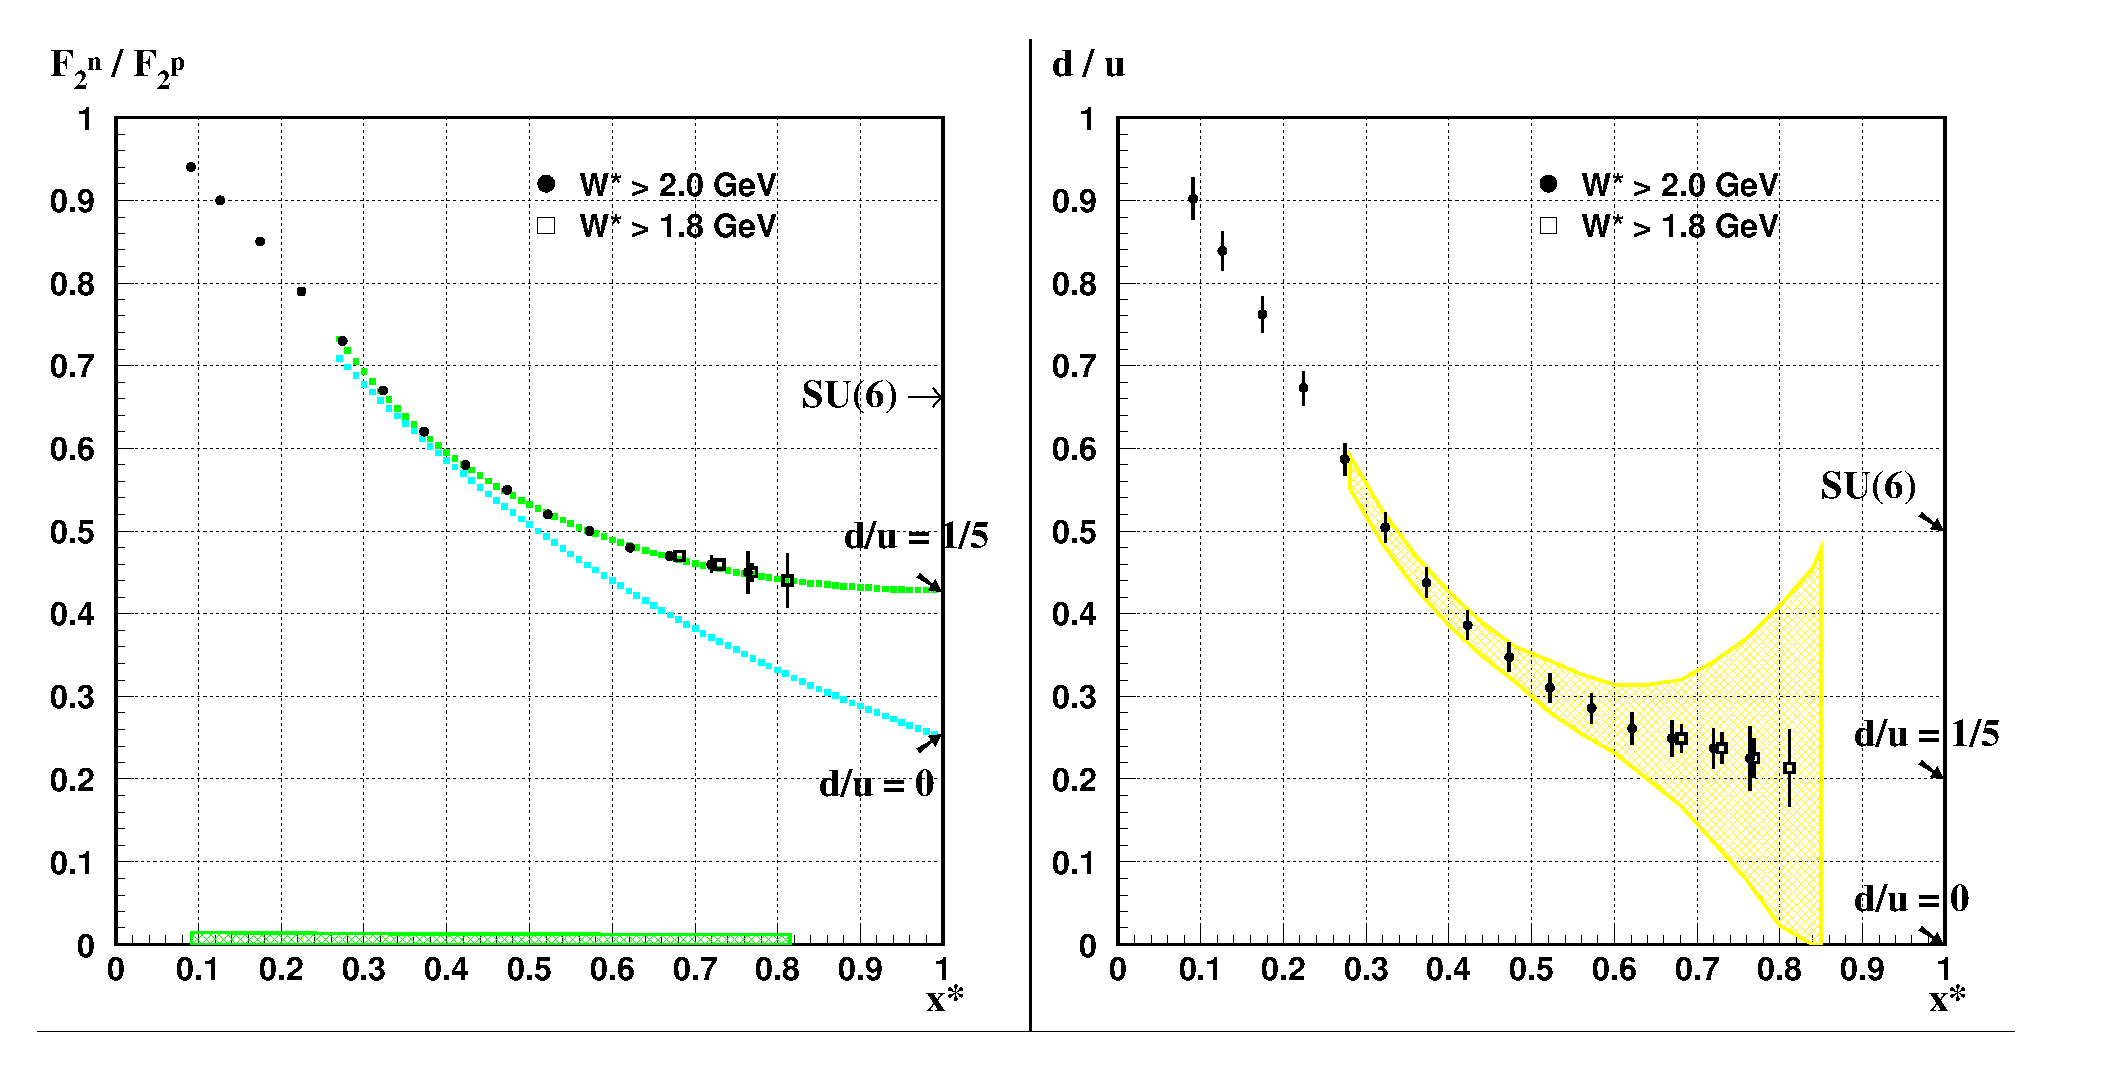
\includegraphics[scale=0.4, angle=0]{../strucfunc/bonus_12_xpctd.eps}}
\end{center}
\vspace*{-1cm}
\caption{\small{Anticipated results on $F_2^n/F_2^p$ (left) and the extracted 
$u/d$ ratio (right) for 40~days of data taking at 11~GeV with {\tt CLAS12}.  
The arrows along the ordinate indicate model predictions.  The error bars 
pertaining to filled circles are statistical with a $W>2$~GeV constraint.  
The smaller errors (with open squares) are for $W>1.8$~GeV.  The systematic 
error is indicated by the band along the abscissa on the left plot.  The two 
curves on the left plot represent hadron-parton duality based predictions 
with two different mechanisms for SU(6) symmetry breaking. The shaded band 
on the right plot indicates our present knowledge on the $d/u$ ratio.}}
\label{fig:b12xpctd}
\end{figure}
%%%%%%%%%%%%%%%%%%%%%%%%%%%%%%%%%%%%%%%%%%%%%%%%%%%%%%%%%%%%%%%%%%%%%%%%%%%

JLab PAC30 also approved E12-06-109 \cite{EG12} which will, in particular,
study polarized parton distributions at large $x$. Using standard detection 
equipment, a redesigned polarized target adapted to {\tt CLAS12} and 30 
(50)~days of running on a longitudinally polarized NH$_3$ (ND$_3$) target, 
high precision measurements can be achieved as shown in Fig.~\ref{fig:A1xpctd}. 
These data will disentangle models in the large-$x$ region.  While the results 
shown in Fig.~\ref{fig:A1xpctd} are with a $W>2$~GeV constraint, hadron-parton 
duality studies (see page \pageref{duality}) will tell us by how much this 
constraint can be relaxed, possibly increasing the $x$ range up to 0.9.  The 
expected accuracy for $(\Delta d+ \Delta\bar{d})/(d+\bar{d})$ is 
shown in Fig.~\ref{fig:ddodxpctd}.
 
%%%%%%%%%%%%%%%%%%%%%%%%%%%%%%%%%%%%%%%%%%%%%%%%%%%%%%%%%%%%%%%%%%%%%%%%%%%
\begin{figure}[ht!]
\begin{center}
\centerline{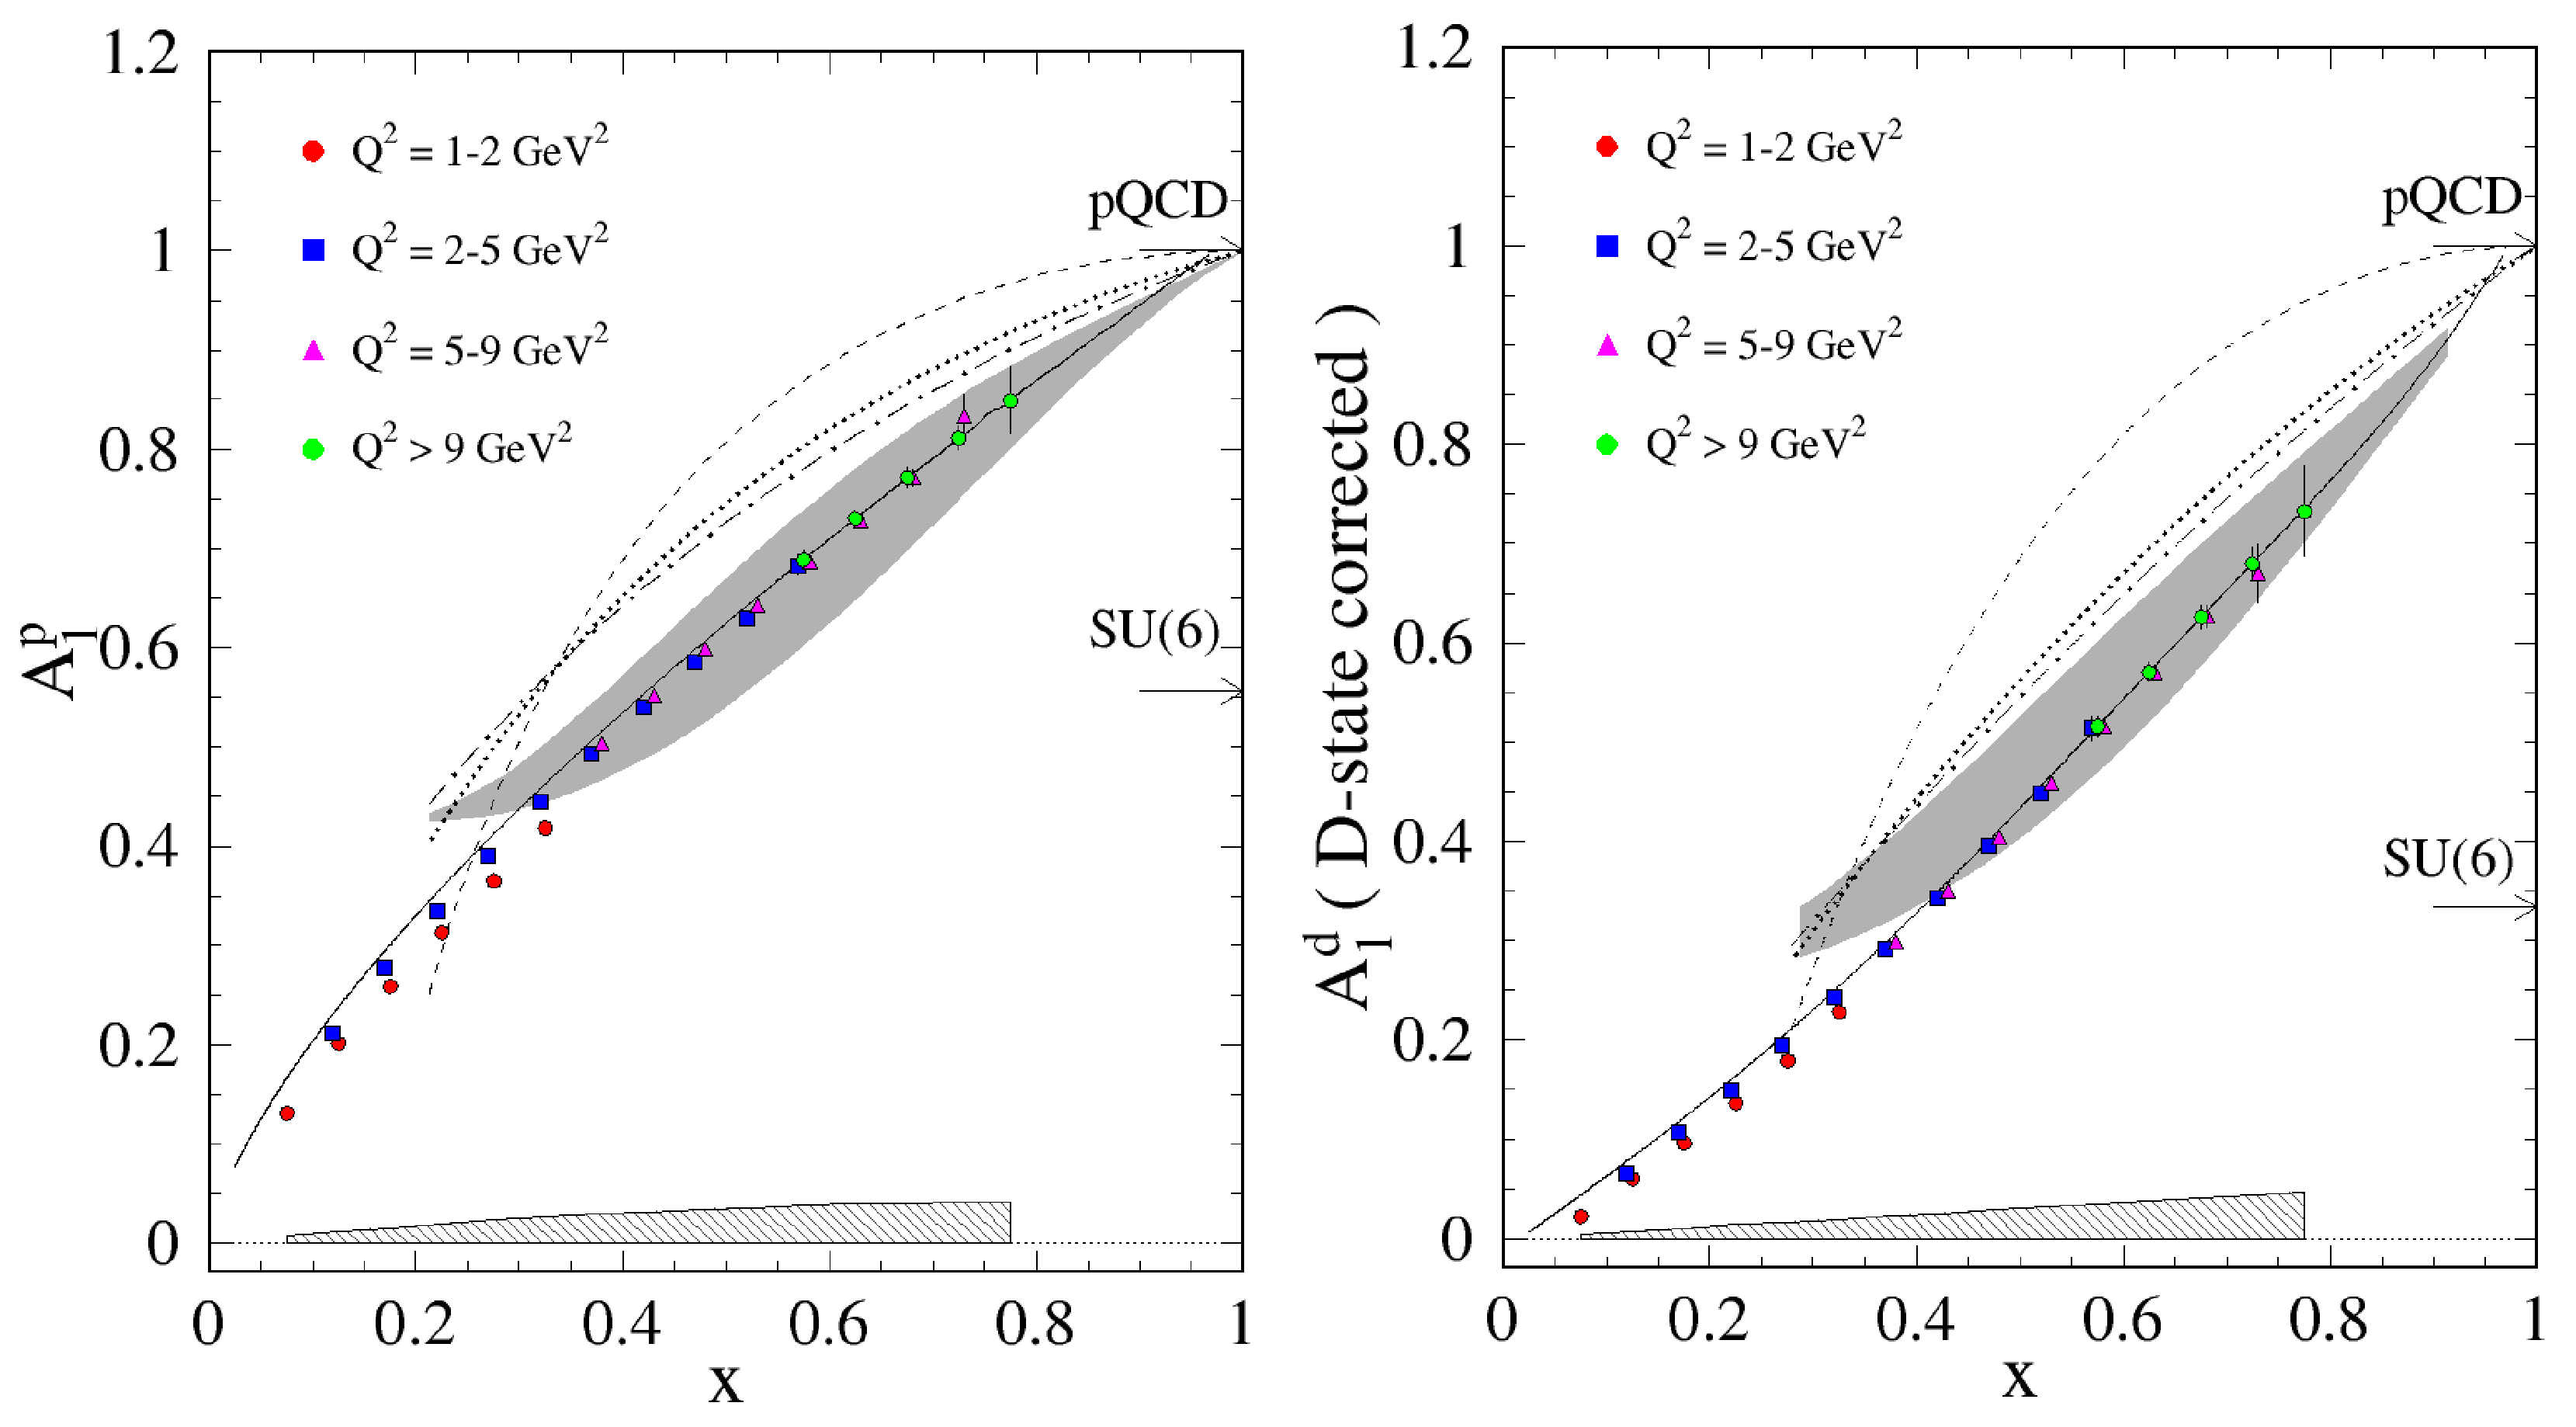
\includegraphics[scale=0.25, angle=0]{../strucfunc/A1_xpctd.eps}}
\end{center}
\vspace*{-1cm}
\caption{\small{Anticipated results on $A_1^p$ (left) and $A_1^d$ (right).
The four different symbols represent four different $Q^2$ ranges.  The 
statistical uncertainty is given by the error bars while the systematic 
uncertainty is given by the shaded band.}}
\label{fig:A1xpctd}
\end{figure}
%%%%%%%%%%%%%%%%%%%%%%%%%%%%%%%%%%%%%%%%%%%%%%%%%%%%%%%%%%%%%%%%%%%%%%%%%%%

%%%%%%%%%%%%%%%%%%%%%%%%%%%%%%%%%%%%%%%%%%%%%%%%%%%%%%%%%%%%%%%%%%%%%%%%%%%
\begin{figure}
\begin{center}
\begin{minipage}[t]{0.55\linewidth}
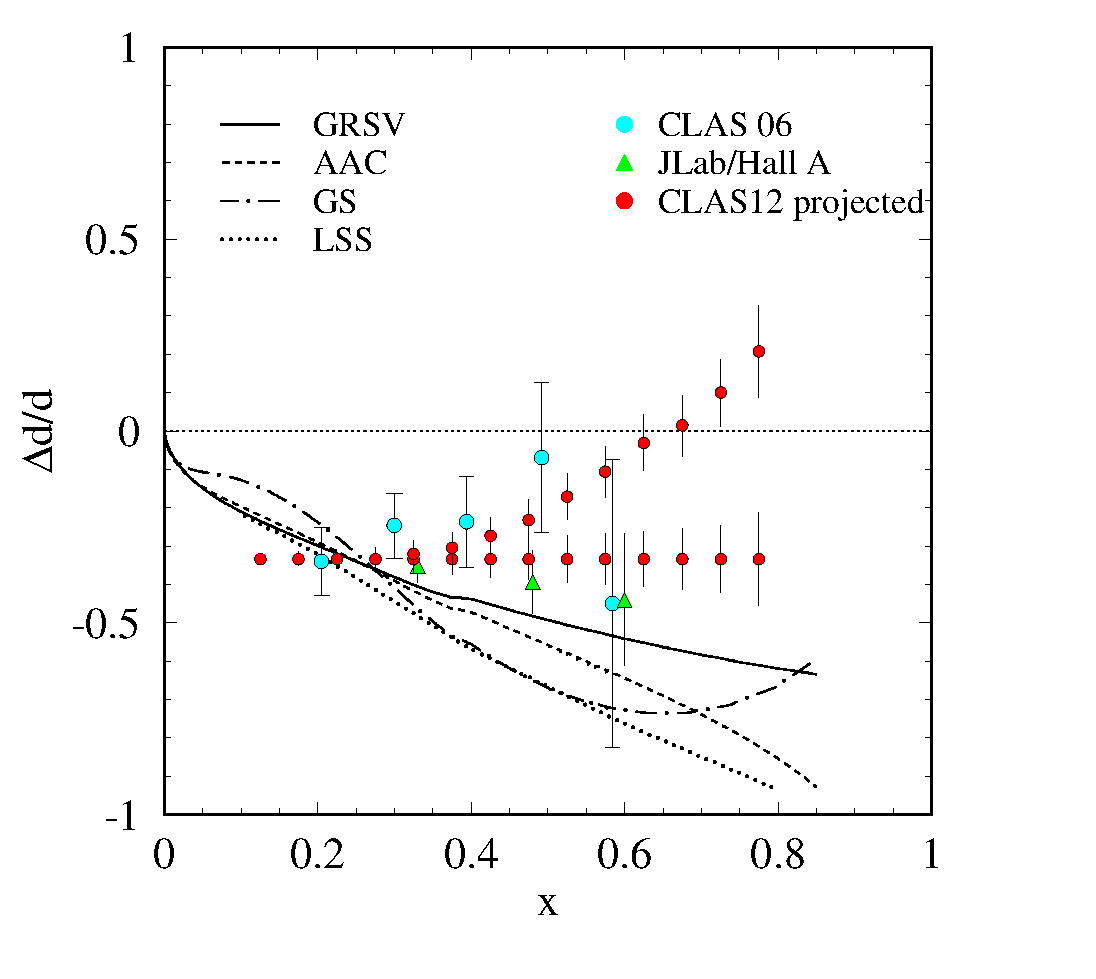
\includegraphics[scale=0.5, angle=0]{../strucfunc/ddod_xpctd.eps}
\end{minipage}\hfill
\begin{minipage}[c]{0.45\linewidth}
\vspace*{-9cm}
\caption{\small{Expected results for $(\Delta d+ \Delta\bar{d})/(d+\bar{d})$. 
The central values of the data are following two arbitrary curves to 
demonstrate how the two categories of predictions, namely the ones that 
predict $\Delta d/d$ stays negative (LO and NLO analyses of polarized 
DIS data: GRSV, LSS, AAC, GS, statistical model, and a quark-hadron duality 
scenario) and the ones predicting $\Delta d/d \to 1$ when $x \to 1$ (leading 
order pQCD and a quark-hadron duality scenario).}}
\label{fig:ddodxpctd}
\end{minipage}
\end{center}
\end{figure}
%%%%%%%%%%%%%%%%%%%%%%%%%%%%%%%%%%%%%%%%%%%%%%%%%%%%%%%%%%%%%%%%%%%%%%%%%%%


\section{Global Fit of Polarized Parton Distributions}

The large window opened by the 12-GeV upgrade over the DIS domain will permit 
constraints of global fits of the parton distributions.  The unique impact at 
large $x$ has just been discussed.  The improvement from the 12-GeV upgrade is 
also significant at low and moderate $x$, noticeably for the polarized gluon 
distribution $\Delta G$.  For a more complete picture of the precision 
achievable with the expected {\tt CLAS12} data, we have plotted in 
Fig.~\ref{pPDFs_exp} an analysis of the impact on NLO analyses.  A dramatic 
improvement can be achieved with the expected data from the {\tt CLAS12} 
proposal E12-06-109~\cite{EG12}.  We emphasize that the data will not only 
reduce the error band on $\Delta G$, but will likely allow a more detailed 
modeling of its $x$-dependence.

%%%%%%%%%%%%%%%%%%%%%%%%%%%%%%%%%%%%%%%%%%%%%%%%%%%%%%%%%%%%%%%%%%%%%%%%%%%
\begin{figure}[htbp]
\vspace{8.5cm}
\special{psfile=../strucfunc/Delu_LSS.eps hscale=55 vscale=55 hoffset=45 voffset=150}
\special{psfile=../strucfunc/Deld_LSS.eps hscale=55 vscale=55 hoffset=245 voffset=150}
\special{psfile=../strucfunc/Delg_LSS.eps hscale=55 vscale=55 hoffset=45 voffset=0}
\special{psfile=../strucfunc/Dels_LSS.eps hscale=55 vscale=55 hoffset=245 voffset=0}
\caption{\small{Expected uncertainties for $\Delta u$, $\Delta d$, $\Delta G$,
and $\Delta s$ from an NLO analysis of all world data.  The outermost line 
shows the result from the analysis by Leader, Sidorov, and Stamenov
\protect{\cite{Leader:2005ci}}.  The second line is the updated result after 
inclusion of the new EG1b data from {\tt CLAS} at 5.7~GeV
\protect{\cite{Dharmawardane:2006zd}}.  The innermost line shows the expected 
uncertainty after including the data set to be collected with {\tt CLAS12}, 
including statistical and systematic errors.}}
\label{pPDFs_exp}
\end{figure}
%%%%%%%%%%%%%%%%%%%%%%%%%%%%%%%%%%%%%%%%%%%%%%%%%%%%%%%%%%%%%%%%%%%%%%%%%%%

 
\section{Moments of Structure Functions}

Moments of structure functions provide powerful insight into nucleon 
structure.  Inclusive data at JLab have permitted evaluation of the moments 
at low and intermediate $Q^2$~\cite{Fatemi:2003yh,Yun:2002td,Chen:2005td}.  
With a maximum beam energy of 6~GeV, however, the measured strength of the 
moments becomes rather limited for $Q^2$ greater than a few GeV$^2$. The 
12-GeV upgrade removes this problem and allows for measurements to higher 
$Q^2$. 

Moments of structure functions can be related to the nucleon static properties 
by sum rules. At large $Q^2$ the Bjorken sum rule relates $\int g_1^{p-n} dx$ 
to the nucleon axial charge~\cite{Bjorken:1966jh}.  At the other end of the 
spectrum, $Q^2$ = 0, the Gerasimov-Drell-Hearn (GDH) sum rule links the 
difference of spin dependent cross sections, integrated over photon energy, 
to the anomalous magnetic moment of the nucleon~\cite{Drell:1966jv,
Gerasimov:1965et}.  The two sum rules are aspects of a general one derived 
recently by Ji and Osborne~\cite{Ji:1999mr} that is valid at any $Q^2$
and links the first moments of spin structure functions to spin-dependent 
Compton amplitudes. Low $Q^2$ is a testing ground for chiral perturbation 
theory, while large $Q^2$ data can be compared to higher-twist series derived 
within the operator product expansion (OPE) method.  Lattice QCD can calculate 
higher-twist terms, thus extending the validity domain of OPE to lower $Q^2$. 
However OPE is unusable at low $Q^2$.  To bridge the gap, lattice QCD can be 
used to compute Compton amplitudes at any $Q^2$.  Hence, the Ji and Osborne 
sum rule can be computed and compared to experiments at any $Q^2$, making it a 
unique tool to study the transition from partonic to hadronic degrees of 
freedom.

%%%%%%%%%%%%%%%%%%%%%%%%%%%%%%%%%%%%%%%%%%%%%%%%%%%%%%%%%%%%%%%%%%%%%%%%%%
\begin{figure}[htb]
\centerline{\epsfxsize=5in\epsfbox{../strucfunc/expect.eps}}
\caption{\small{Left plot: expected precision on $\Gamma_1^p$ for {\tt CLAS12}
and 30~days of running.  {\tt CLAS} EG1a~\cite{Fatemi:2003yh, Yun:2002td} data 
and preliminary results from EG1b are shown for comparison.  The data and 
systematic uncertainties do not include estimates of the unmeasured DIS 
contribution.  HERMES~\cite{Airapetian:2002wd} data, and E143~\cite{Abe:1998wq} 
and E155 data~\cite{Anthony:2000fn} from SLAC are also shown (including DIS 
contribution estimates).  The model is from Burkert and Ioffe
\cite{Burkert:1992tg,Burkert:1993ya}.  Right plot: same as the left but 
including an estimate of the DIS contribution.}}
\label{expect}
\end{figure}
%%%%%%%%%%%%%%%%%%%%%%%%%%%%%%%%%%%%%%%%%%%%%%%%%%%%%%%%%%%%%%%%%%%%%%%%%%

The left plot in Fig.~\ref{expect} shows the expected precision on the 
measured part of $\Gamma_1^p$.  The inner error bar is statistical while the 
outer one is the statistics and systematics added in quadrature.  Published 
results and preliminary results from EG1b are also displayed for comparison. 
Like the {\tt CLAS12} data, the EG1 data do not include the unmeasured DIS 
contribution.  The hatched blue band corresponds to the systematic uncertainty 
on the EG1b data points.  The red band indicates the estimated systematic 
uncertainty from {\tt CLAS12}.  The right plot in Fig.~\ref{expect} shows the 
results on $\Gamma_1^p$ and $\Gamma_1^d$ including an estimate of the 
unmeasured DIS contribution.  The systematic uncertainties for EG1 and 
{\tt CLAS12} here include the estimated uncertainty on the unmeasured DIS part 
estimated using the model from Bianchi and Thomas~\cite{Thomas:2000pf}.  As 
can be seen, moments can be measured up to $Q^2$=6~GeV$^2$ with a statistical 
accuracy improved several fold over that of the existing world data.

Higher moments are also of interest: generalized spin polarizabilities
are linked to higher moments of spin structure functions by sum rules based 
on similar grounds as the GDH sum rule. Higher moments are less sensitive to 
the unmeasured low-$x$ part, so measurements are possible up to higher $Q^2$ 
compared to first moments.  Just like the GDH/Bjorken sum rules, measurements 
of the $Q^2$-evolution allow us to study the parton-hadron transition since 
theoretical predictions exist at low and large $Q^2$~\cite{Chen:2005td}.  In 
addition, spin polarizabilities are also fundamental observables characterizing 
the nucleon structure and the only practical way known to measure them is 
through measurement of moments and application of the corresponding sum rules.

Finally, moments in the low ($\simeq$ 0.5 GeV$^2$) to moderate 
($\simeq$4~GeV$^2$) $Q^2$ range enable us to extract higher-twist parameters,
which represent correlations between quarks in the nucleon.  This extraction 
can be done by studying the $Q^2$ evolution of first moments~\cite{Chen:2005td}.
Higher twists have been consistently found to have, overall, a surprisingly 
smaller effect than expected.  Going to lower $Q^2$ enhances the higher-twist 
effects but makes it harder to disentangle a high twist from the yet higher 
ones.  Furthermore, the uncertainty on $\alpha _s$ becomes prohibitive at low 
$Q^2$.  Hence, higher twists turn out to be hard to measure, even at the 
present JLab energies.  Adding higher $Q^2$ to the present JLab data set 
removes the issues of disentangling higher twists from each other and of the 
$\alpha _s$ uncertainty.  The smallness of higher twists, however, requires 
statistically precise measurements with small point-to-point correlated 
systematic uncertainties.  Such precision at moderate $Q^2$ has not been 
achieved by the experiments done at high energy accelerators, while JLab at 
12~GeV presents the opportunity to reach it considering the expected 
statistical and systematic uncertainties of E12-06-109.  The total 
point-to-point uncorrelated uncertainty on the twist-4 term for the Bjorken 
sum, $f_2^{p-n}$, decreases by a factor of 5.6 compared to results obtained in
Ref.~\cite{Deur:2004ti}. 

\subsection{The GDH Sum Rule}

Despite its fundamental nature, the GDH sum rule has not yet been fully 
verified experimentally.  Combined results from MAMI and ELSA~\cite{GDH04}
are about 10\% above the expected value.  This is for an upper integration 
limit in photon energy of about 2.8~GeV.  With the cancellation of the fixed 
target program at SLAC and consequently of experiment E159~\cite{SLACGDH} that 
would have investigated the GDH strength at large $\nu$, JLab is now the best 
place to test the convergence of the GDH sum.  Using real photons or 
near real photons, we can measure the contribution to the GDH sum rule up to 
10.5~GeV, about 4 times the maximum energy reached at ELSA (see 
Fig.~\ref{gdhf}).  A non-convergence of the sum rule would be intriguing 
and may signal physics beyond the Standard Model.  In any case it will provide 
important insight on soft Regge physics.

%%%%%%%%%%%%%%%%%%%%%%%%%%%%%%%%%%%%%%%%%%%%%%%%%%%%%%%%%%%%%%%%%%%%%%%%%%
\begin{figure}
\begin{center}
\begin{minipage}[t]{0.6\linewidth}
\centerline{\epsfxsize=4.in\epsfbox{../strucfunc/gdhprev.eps}}
\end{minipage}\hfill
\begin{minipage}[c]{0.35\linewidth}
\vspace*{-7cm}
\caption{\small{Coverage of the GDH sum rule for low-$Q^2$ experiments with 
{\tt CLAS} and {\tt CLAS12}.  The data points are the GDH running sum from 
MAMI and ELSA at $Q^2=0$.}}
\label{gdhf}
\end{minipage}
\end{center}
\end{figure}
%%%%%%%%%%%%%%%%%%%%%%%%%%%%%%%%%%%%%%%%%%%%%%%%%%%%%%%%%%%%%%%%%%%%%%%%%%

\subsection{Moments of $F_2$ and the Precise Determination of $\alpha_s(M_Z)$}

Simulated results for the moments $\int x^n F_2 dx$  with $n \leq 8$ are 
shown in Fig.~\ref{fig:moments}.  It reveals that {\tt CLAS12} will provide 
a unique tool to extract moments of $F_2$ up to $Q^2$ values of 
10 - 14~GeV$^2$.  These can be used to extract the strong coupling constant 
$\alpha_{s}(M_{z})$.  The extraction of $\alpha_s(M_Z)$ from the scaling 
violations of the proton structure function $F_2$ is one of the most precise 
methods available up to now (see Fig.~\ref{fig:alpha}).  Simulation shows that 
a new procedure for the extraction of $\alpha_s(M_Z)$~\cite{Simula:2003vf} 
together with the {\tt CLAS12} data can allow an unprecedentedly accurate 
determination of $\alpha_s(M_Z)$ with a statistical uncertainty of 0.0008 and 
a systematic uncertainty of about 0.0007.

%%%%%%%%%%%%%%%%%%%%%%%%%%%%%%%%%%%%%%%%%%%%%%%%%%%%%%%%%%%%%%%%%%%%%%%%%%
\begin{figure}[htbp]
\vspace{8.0cm}
\special{psfile=../strucfunc/fig_moments.ps hscale=45 vscale=45 hoffset=100 voffset=-70}
\caption{\small{Expected moments of the proton structure function $F_2$ 
obtained with the {\tt CLAS12} detector simulations for a few days of 
running.  The meaning of the markers and the scale factors for each moment 
are indicated in the inset.}}
\label{fig:moments} 
\end{figure}
%%%%%%%%%%%%%%%%%%%%%%%%%%%%%%%%%%%%%%%%%%%%%%%%%%%%%%%%%%%%%%%%%%%%%%%%%%

%%%%%%%%%%%%%%%%%%%%%%%%%%%%%%%%%%%%%%%%%%%%%%%%%%%%%%%%%%%%%%%%%%%%%%%%%%
\begin{figure}[htbp]
\vspace{10.5cm}
\special{psfile=../strucfunc/alpha_s.epsi hscale=65 vscale=62 hoffset=30 voffset=-100}
\caption{\small{Existing determinations of the QCD coupling constant 
$\alpha_S(M_Z)$~\cite{alpha}.}}
\label{fig:alpha} 
\end{figure}
%%%%%%%%%%%%%%%%%%%%%%%%%%%%%%%%%%%%%%%%%%%%%%%%%%%%%%%%%%%%%%%%%%%%%%%%%%


\subsection{Quark-Hadron Duality} 
\label{duality}

The phenomenon of quark-hadron duality relates the physics of nucleon 
resonances to the dynamics of single quark scattering that governs the 
scaling structure functions at high energy.  JLab measurements of the 
unpolarized proton structure functions in the resonance region 
\cite{Niculescu:2000tk,ERIC} have sparked considerable interest in 
quark-hadron duality~\cite{Bloom:1970xb,Bloom:1971ye,DeRujula:1976tz,
Isgur:2001bt}.  While quark-hadron duality has been observed in the
spin-independent $F_2$ structure function~\cite{Bloom:1970xb,Bloom:1971ye,
Niculescu:2000tk}, it has not yet been firmly established for spin-dependent 
structure functions.  Because the $g_1$ structure function is given by a 
difference of cross sections, which need not be positive, the workings of 
duality will necessarily be more intricate for $g_1$ than for the
spin-averaged $F_2$ structure function.  The first results from the spin 
structure function measurements in Hall A~\cite{Amarian:2003jy,E01-012} and 
with {\tt CLAS}~\cite{Bosted:2006gp} indicate that, if one averages over 
the entire resonance region, duality roughly holds for $Q^2$ above 
1.5~GeV$^2$. To achieve a more precise understanding of the mechanism of 
duality, it is necessary to determine the conditions under which duality 
occurs in both polarized and unpolarized structure functions.  An upgraded 
{\tt CLAS12} would permit measurements of the structure functions in the 
DIS region with high precision.  For unpolarized parton distributions, the 
tagging technique used by the BONUS experiment~\cite{BONUS} (see 
Section~\ref{F2A1}) can also be applied to the neutron resonance region, 
where at present there are essentially no data.



%
\chapter{SIDIS and the Transverse Structure of the Nucleon}

\section{Introduction}

The spin structure of the nucleon has been of particular interest since the 
EMC~\cite{Ashman:1987hv} measurements implied that the helicity of the 
constituent quarks account for only a fraction of the nucleon spin.  The 
so-called ``spin crisis'' was subsequently confirmed by a number of other 
experiments at CERN~\cite{Adams:1997tq}, SLAC~\cite{Abe:1998wq,Anthony:1999py},
HERA~\cite{Ackerstaff:1999ey,Airapetian:2004zf}, and JLab~\cite{Fatemi:2003yh}.
Possible interpretations of this result include the contribution of the
orbital momentum of quarks and significant polarization of either the strange 
sea (negatively polarized) or gluons (positively polarized).  The 
contributions to the sum rule for the total helicity of the nucleon
include the following:

\begin{equation}
\frac{1}{2} = \frac{1}{2} \sum_q \Delta q^{val} + \Delta q^{sea}
+L_z^{val} + L_z^{sea} + L_z^{glue} + \Delta G,
\label{angmom_sumrule_a}
\end{equation}

\noindent
where $\Delta q$, $L_z$, and $\Delta G$ are respectively the quark helicity, 
the orbital angular momentum of all partons, and the gluon helicity.

Present knowledge about the spin structure of the nucleon comes mainly from 
polarized deep inelastic scattering (DIS). The polarization of the individual 
flavors and anti-flavors were mainly studied using fits to the inclusive data.
Inclusive DIS is sensitive to only the squared charges of the partons, 
and requires additional assumptions ({\it e.g.} an SU(3) symmetric sea), 
which leads to certain ambiguities.  Semi-inclusive deep inelastic scattering
(SIDIS) studies, when a hadron is detected in coincidence with the scattered 
lepton that allows so-called ``flavor tagging'', provide more direct access to 
contributions from various quarks.  In addition, they give access to the 
transverse momentum distributions of quarks, not accessible in inclusive 
scattering.  Azimuthal distributions of final state particles in semi-inclusive 
deep inelastic scattering  provide access to the orbital motion of quarks and 
play an important role in the study of transverse momentum distributions of 
quarks in the nucleon.

Significant progress has been made recently in understanding the role of 
partonic initial and final state interactions~\cite{Brodsky:2002cx,
Collins:2002kn,Ji:2002aa}.  The interaction between the active parton in
the hadron and the spectators leads to gauge-invariant transverse momentum 
dependent (TMD) parton distributions~\cite{Brodsky:2002cx,Collins:2002kn,
Ji:2002aa,Belitsky:2002sm,Boer:2003cm}.  Furthermore, QCD factorization for 
semi-inclusive deep inelastic scattering at low transverse momentum in the 
current-fragmentation region has been established in Refs.~\cite{Ji:2004wu,
Collins:2004nx}.  This new framework provides a rigorous basis to study the 
TMD parton distributions from SIDIS data using different spin-dependent and 
independent observables.  TMD distributions (see Table~\ref{tab1}) describe 
transitions of a nucleon with one polarization in the initial state to a 
quark with another polarization in the final state.

The diagonal elements of the table are the momentum, longitudinal and 
transverse spin distributions of partons, and represent well-known parton
distribution functions related to the square of the leading-twist, light-cone 
wave functions. Off-diagonal elements require non-zero orbital angular 
momentum and are related to the wave function overlap of $L$=0 and $L$=1 Fock 
states of the nucleon~\cite{Ji:2002xn}.  The chiral-even distributions 
$f_{1T}^\perp$ and $g_{1T}$ are the imaginary parts of the corresponding
interference terms, and the chiral-odd $h_1^\perp$ and $h_{1L}$ are the
real parts.  The TMDs $f_{1T}^\perp$ and  $h_{1}^\perp$, which are related to 
the imaginary part of the interference of wave functions for different orbital 
momentum states and are known as the Sivers and 
Boer-Mulders functions~\cite{Sivers:1990fh,Anselmino:1998yz,Brodsky:2002rv,
Collins:2002kn,Ji:2002aa,Belitsky:2002sm}, describe unpolarized quarks in the 
transversely polarized nucleon and transversely polarized quarks in the 
unpolarized nucleon respectively.  They vanish at tree-level in a $T$-reversal 
invariant model ($T$-odd) and can only be non-zero when initial or final state 
interactions cause an interference between different helicity states.  This 
function parameterizes the correlation between the transverse momentum of 
quarks and the spin of a transversely polarized target or the transverse spin 
of the quark, respectively.  They require both orbital angular momentum, as 
well as non-trivial phases from the final state interaction, that survive in 
the Bjorken limit.  Experimental results on the Sivers functions for up and 
down quarks so far are consistent with a heuristic model of up and down quarks 
orbiting  the nucleon in opposite directions.  The most simple mechanism that 
can lead to a Boer-Mulders function is a correlation between the spin of the 
quarks and their orbital angular momentum.  In combination with a final state 
interaction that is on average attractive, already a measurement of the sign 
of the Boer-Mulders function, would thus reveal the correlation between 
orbital angular momentum and spin of the quarks. 

%%%%%%%%%%%%%%%%%%%%%%%%%%%%%%%%%%%%%%%%%%%%%%%%%%%%%%%%%%%%%%%%%%%%%%%%%%%%%
\begin{table}
\begin{center}
\begin{tabular}{|c|c|c|c|} \hline\hline
N/q & U & L & T \\ \hline
 {U} & ${\color{blue} \bf f_1}$   & & ${\color{red} h_{1}^\perp}$ \\
\hline
 {L} & &${\color{green} \bf g_1}$ &    ${\color{red} h_{1L}^\perp}$ \\
\hline
 {T} & ${\color{blue} f_{1T}^\perp} $ &  ${\color{green} g_{1T}}$ &  ${\color{red} \bf h_1}$ \, ${\color{red} h_{1T}^\perp }$ \\
\hline\hline
\end{tabular}
\end{center}
\caption{\small{{Leading-twist transverse momentum-dependent distribution 
functions.  $U$, $L$, and $T$ stand for transitions of unpolarized, 
longitudinally polarized, and transversely polarized nucleons (rows) to 
corresponding quarks (columns).}}
\label{tab1}} 
\end{table}
%%%%%%%%%%%%%%%%%%%%%%%%%%%%%%%%%%%%%%%%%%%%%%%%%%%%%%%%%%%%%%%%%%%%%%%%%%%%%

The impact parameter space displacement of transversely polarized quark 
distributions in an unpolarized target is described by a chirally odd GPD 
\cite{Burkardt:2005hp}, and has recently been calculated for the first time 
in lattice QCD \cite{Gockeler:2005cd,Gockeler:2006zu}. The resulting transverse
flavor dipole moment for transversely polarized quarks in an unpolarized 
nucleon suggests that the Boer-Mulders functions are significantly larger 
than the Sivers functions.  Moreover, consistent with large $N_C$ predictions, 
the displacement of transversely polarized $u$ and $d$ quarks was found to be 
in the same direction, indicating the same sign for the Boer-Mulders functions
for $u$ and $d$ quarks, and suggesting a further enhancement of the
SIDIS asymmetry from the $d$ quark contribution.

Similar quantities arise in the hadronization process.  One particular case 
is the Collins $T$-odd fragmentation function $H_1^{\perp}$ 
\cite{Collins:1992kk} describing fragmentation of transversely polarized 
quarks into unpolarized hadrons.  Parton model analyses 
\cite{Efremov:2002ut,Afanasev:2003ze,Yuan:2003gu,Metz:2004je} of sub-leading 
single-spin asymmetries observed at HERMES 
\cite{Airapetian:1999tv,Airapetian:2006rx} and {\tt CLAS}~\cite{Avakian:2003pk}
lead to the introduction of new twist-3 $T$-odd distribution functions 
\cite{Collins:2004nx,Boer:2003cm}. 

The off-diagonal TMD distributions arise from interference between amplitudes 
with left- and right-handed polarization states, and only exist because of 
chiral symmetry breaking in the nucleon wave function in QCD.  Their study 
therefore provides a new avenue for probing the chiral nature of the partonic 
structure of hadrons.  The universality of the TMD correlation functions has 
been proven, resulting in a sign change for two $T$-odd TMD distributions 
between Drell-Yan and DIS~\cite{Collins:2002kn,Collins:2004nx}, an exciting 
prediction that has to be confirmed by future experiments.

The JLab 12-GeV upgrade will provide the unique combination of wide kinematic 
coverage, high beam intensity (luminosity), high energy, high polarization,
and advanced detection capabilities necessary to study the transverse momentum 
and spin correlations allowing studies of semi-inclusive processes both in the 
target and current fragmentation regions.  The study of the quark 
distributions  in the valence quark region is one of the key objectives of the 
upgrade project~\cite{CDR}.

\section{Present Experimental Results on Spin-Azimuthal Asymmetries}

In recent years, semi-inclusive deep inelastic scattering (SIDIS) has emerged 
as a powerful tool to probe nucleon structure through transverse single spin 
asymmetries (SSAs)~\cite{Airapetian:1999tv,Airapetian:2004tw,Alexakhin:2005iw}.
In contrast to inclusive deep inelastic lepton-nucleon scattering where 
transverse momentum is integrated out, these processes are sensitive to 
transverse momentum scales on the order of the intrinsic quark momentum
$P_T\sim k_\perp$.  Measurements of SSAs in SIDIS provide access to a list of 
novel physics observables including transversity ($h_1$)
\cite{Ralston:1979ys,Jaffe:1991ra}, and the time-reversal odd Sivers 
distribution function ($f_{1T}^\perp$) 
\cite{Sivers:1990fh,Anselmino:1998yz,Brodsky:2002cx,Collins:2002kn,Ji:2002aa}.

For transversely polarized targets, several azimuthal asymmetries already 
arise at leading order.  Four contributions related to the corresponding 
distribution functions were investigated in Refs.~\cite{Collins:1992kk,Mulders:1995dh,Kotzinian:1994dv,Brodsky:2002cx,Ji:2002aa,Kotzinian:1995cz}:

\begin{eqnarray}
\sigma^{\cos\phi}_{LT} &\propto& \lambda_e S_T y (1-y/2) \cos(\phi - \phi_S)\sum_{q,\bar{q}} e^2_q {x g_{1T}^q(x)} {D_1^{q}(z)}, \\
\sigma^{\sin\phi}_{UT}&\propto&             S_T (1-y)\sin(\phi+\phi_S)\sum_{q,\bar{q}} e^2_q {x h_1(x)} {H_1^{\perp q}(z)}  \nonumber  \\
       &+&             S_T (1-y+y^2/2)\sin(\phi-\phi_S)\sum_{q,\bar{q}} e^2_q {x f^{\perp q}_{1T}(x)} {D_1^{q}(z)} \nonumber\\
       &+&             S_T (1-y)\sin(3\phi-\phi_S)\sum_{q,\bar{q}} e^2_q {x h^{\perp q}_{1T}(x)} {H_1^{\perp q}(z)},
\label{sivco} 
\end{eqnarray}

\noindent 
where $\phi$ and $\phi_S$ are the azimuthal angles of the hadron and transverse 
spin in the photon frame, $x,y,z$ define the fractions of the proton momentum
carried by the struck quark, electron momentum carried by the virtual photon.
and the virtual photon momentum carried by the final state hadron, respectively.
$D_1^{q}(z)$ and $H_1^{\perp {q}}(z)$ are the spin-independent and 
spin-dependent fragmentation functions. 

%%%%%%%%%%%%%%%%%%%%%%%%%%%%%%%%%%%%%%%%%%%%%%%%%%%%%%%%%%%%%%%%%%%%%%%%%%%%%
\begin{figure}[tb]
\begin{center}
\vspace{-6.0cm}
\mbox{ 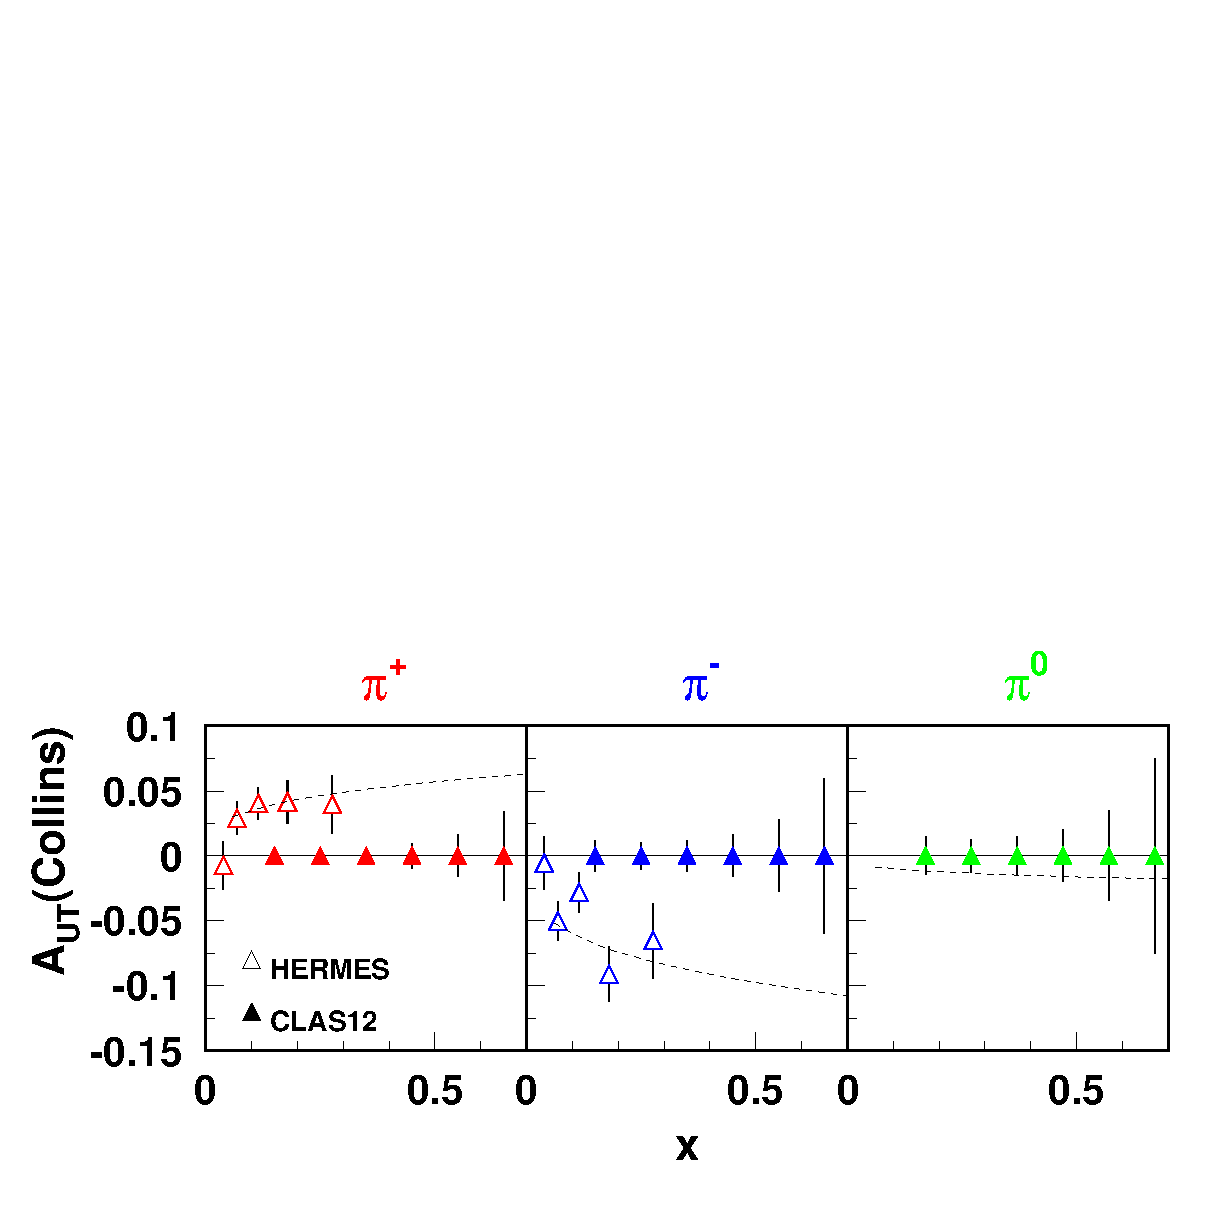
\psfig{file=../sidis/autcollins11.her.eps,height=14cm,width=14.0cm} }
\caption{\small{Projected transverse spin asymmetry from the Collins effect 
($A_{UT}^{\sin(\phi+\phi_S)}$) in single $\pi$ production with {\tt CLAS} at 
11~GeV.}} 
\label{fig:autcol}
\end{center}
\end{figure}
%%%%%%%%%%%%%%%%%%%%%%%%%%%%%%%%%%%%%%%%%%%%%%%%%%%%%%%%%%%%%%%%%%%%%%%%%%%%%

\vspace{0.2cm}\noindent

%%%%%%%%%%%%%%%%%%%%%%%%%%%%%%%%%%%%%%%%%%%%%%%%%%%%%%%%%%%%%%%%%%%%%%%%%%%%
\begin{figure}[tb]
\begin{center}
\vspace{-6.0cm}
\mbox{ 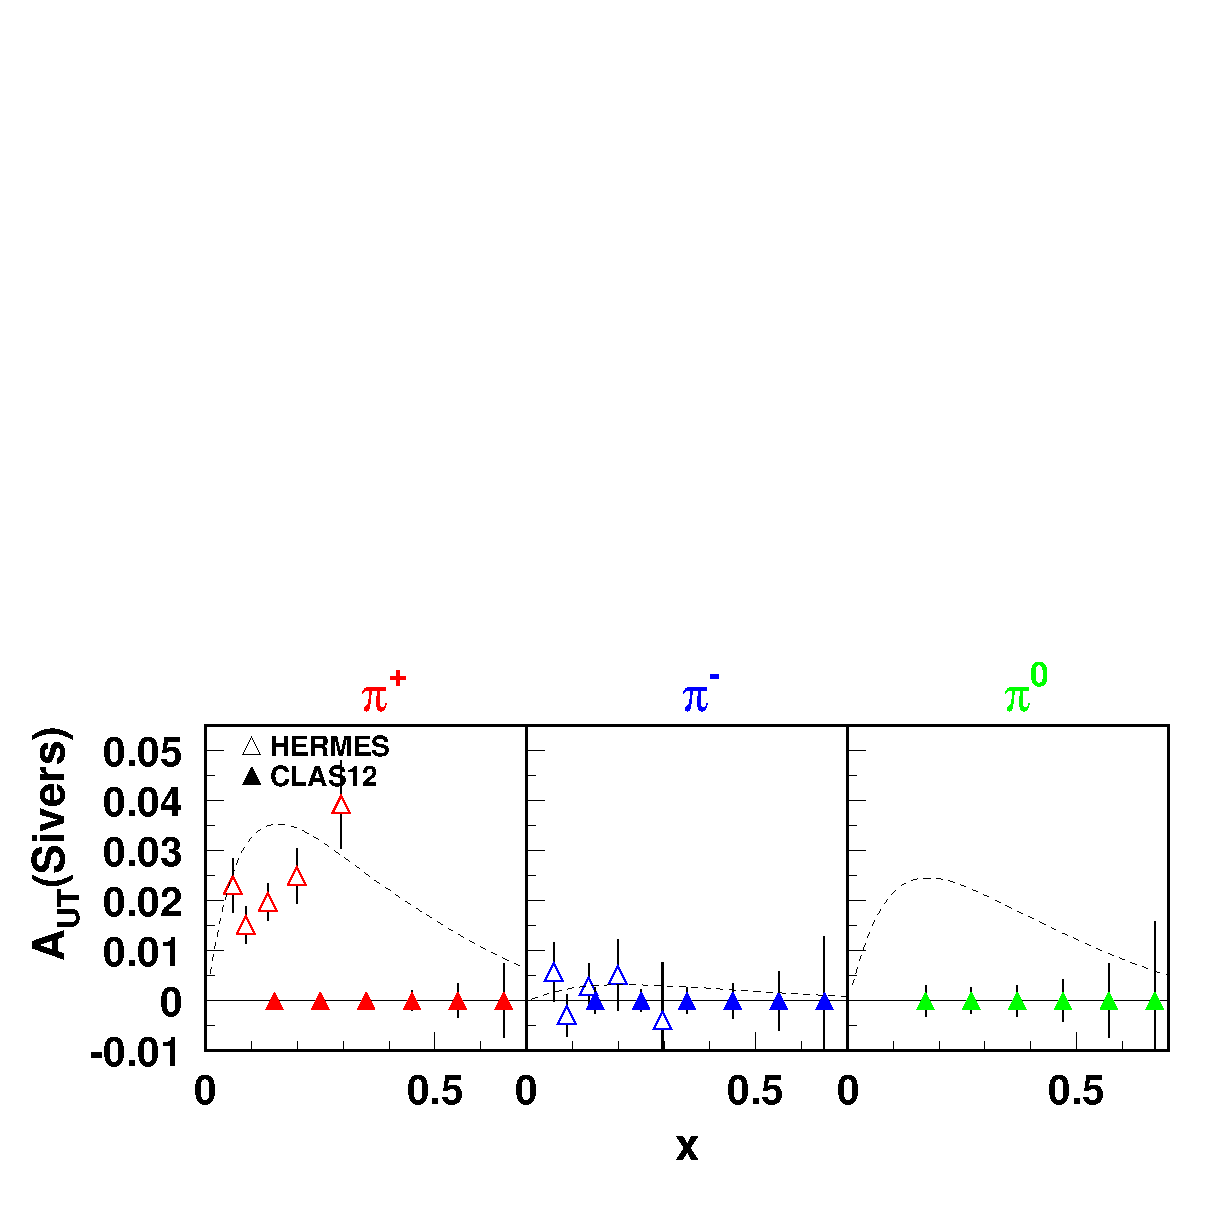
\psfig{file=../sidis/autsivers11.weiss.eps,height=14cm,width=14.0cm} }
\caption{\small{Projected transverse spin asymmetry from the Sivers effect 
($A_{UT}^{\sin(\phi-\phi_S)}$) in single $\pi$ production with {\tt CLAS12} 
at 11~GeV.}}
\label{fig:autsiv}
\end{center}
\end{figure}
%%%%%%%%%%%%%%%%%%%%%%%%%%%%%%%%%%%%%%%%%%%%%%%%%%%%%%%%%%%%%%%%%%%%%%%%%%%%

The leading-twist transversity distribution $h_1$
\cite{Ralston:1979ys,Jaffe:1991ra} and its first moment, the tensor charge, 
are as fundamental for understanding of the spin structure of the nucleon as 
are the helicity distribution $g_1$  and the axial vector charge.  The 
transversity distribution  $h_1$ is charge conjugation odd.  It does not mix 
with gluons and for non-relativistic quarks it is equal to the helicity
distribution $g_1$.  Thus, it probes the relativistic nature of quarks and it 
has a very different $Q^2$ evolution than $g_1$.  The tensor charge is 
reliably calculable in lattice QCD with $\delta \Sigma = \sum_f 
\int_0^1dx(h_1^f - \bar{h_1^f})=0.562 \pm 0.088$ at $Q^2$=2~GeV$^2$, which is 
twice as large as the value of proton axial charge~\cite{Leader:1999rh}.  A 
similar quantity ($\delta \Sigma \approx 0.6$) was obtained in the effective 
chiral quark soliton model~\cite{Kim:1996vk}. 

A detailed study of the $Q^2$ and $x_B$ dependencies as a function of the 
azimuthal angle $\phi$ will allow the separation of contributions from 
different mechanisms.  During the last few years, first results on transverse 
SSAs have become available~\cite{Airapetian:2004tw,Alexakhin:2005iw}. HERMES 
measurements for the first time directly indicated significant azimuthal 
moments generated both by Collins (Fig.~\ref{fig:autcol}) and Sivers 
(Fig.~\ref{fig:autsiv}) effects.

Spin-orbit correlations are also accessible in SIDIS with longitudinally a
polarized target, where they give rise to the Mulders leading-twist 
distribution function $h_{1L}^\perp$. It is related to the real part of
the interference of wave functions for different orbital momentum states,
and describes transversely polarized quarks in the longitudinally polarized 
nucleon.  For a longitudinally polarized target the only azimuthal asymmetry
arising in leading order is the $\sin2\phi$ moment,

\begin{equation}
\sigma^{\sin2\phi}_{UL} \propto S_L 2(1-y)\sin 2\phi\sum_{q,\bar{q}} e^2_q {x h^{\perp q}_{1L}(x)} {H_1^{\perp q}(z)}.
\end{equation}

The physics of $\sigma_{UL}$, which involves the Collins fragmentation 
function $H_1^\perp$ and Mulders distribution function $h_{1L}^\perp$, 
was first discussed by Kotzinian and Mulders in 1996 
\cite{Mulders:1995dh,Kotzinian:1994dv,Kotzinian:1995cz}.  The same 
distribution function is accessible in double polarized Drell-Yan, where it 
gives rise to the $\cos2\phi$ azimuthal moment in the cross section 
\cite{Tangerman:1994eh}.

Measurements of the $\sin2\phi$ SSA \cite{Kotzinian:1995cz}, thus allow the 
study of the Collins effect with no contamination from other mechanisms.  A 
recent measurement of the $\sin 2\phi$ moment of $\sigma_{UL}$ by HERMES 
\cite{Airapetian:1999tv} is consistent with zero.  A measurably large 
asymmetry has been predicted only at large $x$ ($x>0.2$), a region 
well-covered by JLab~\cite{Efremov:2002ut}. 

The kinematic dependence of the SSA for $\pi^+$, measured from the {\tt CLAS} 
EG1 data set at 6~GeV is consistent with predictions~\cite{Efremov:2002ut}. 
The $\pi^+$ SSA is dominated by the $u$-quarks; therefore with some assumption 
about the ratio of unfavored to favored Collins fragmentation functions, it can 
provide a first glimpse of the twist-2 Mulders TMD function.  The distribution 
function $h_{1L}^\perp$ was extracted using the $\pi^+$ target SSA 
\cite{Avakian:2005ps}, which is less sensitive to the unknown ratio of 
unfavored ($d$-quark fragmenting to $\pi^+$) to favored ($u$-quark fragmenting 
to $\pi^+$) polarized fragmentation functions (see Fig. \ref{fig:aul11.sin2}). 
The curve is the result of the calculation by Efremov {\it et al.} 
\cite{Efremov:2002ut}, using $h_{1L}^\perp$ from the chiral quark soliton 
model evolved to $Q^2$=1.5~GeV$^2$.  The extraction, however, suffers from low 
statistics and has a significant systematic error from the unknown ratio of 
the Collins favored and unfavored fragmentation functions, the unknown ratio 
of $h_{1L}^d/h_{1L}^u$, as well as from background from exclusive vector mesons.
Current statistical errors for $\pi^-$, and in particular $\pi^0$, which is 
relatively free of possible higher twist contributions \cite{Afanasev:1996mj},
are large and do not allow strong conclusions from the measured SSAs.  More 
data are required for a statistically significant measurement of the
$\sin2\phi$ moment.

The only leading-twist contribution to the unpolarized target cross section
depending on the azimuthal angle has a term with the Boer-Mulders function 
coupling to the Collins function~\cite{Collins:1992kk}:

\begin{equation}
\sigma^{\cos2\phi}_{UU} \propto 2(1-y)\cos 2\phi\sum_{q,\bar{q}} 
e^2_q {x h^{\perp q}_{1}(x)} {H_1^{\perp q}(z)}.
\end{equation}

The physics of $\sigma^{\cos2\phi}_{UU}$, which involves the Collins 
fragmentation function $H_1^\perp$ and the Boer-Mulders distribution function 
$h_{1}^\perp$, was first discussed by Boer and Mulders in 1998
\cite{Boer:1997nt}.  In recent years, the $\cos 2\phi$ asymmetry in 
leptoproduction was phenomenologically studied using different approximations 
for the Boer-Mulders function 
\cite{Oganesian:1997jq,Gamberg:2003ey,Barone:2005kt}.

Independent information on the Boer-Mulders function 
$h_1^{\perp}(x, \Vec k_T^2)$ can be obtained from the study of the $\cos 2\phi$
azimuthal asymmetry in unpolarized Drell-Yan processes, which has been
measured in $\pi N$ collisions~\cite{Falciano:1986wk,Conway:1989fs}.
In Refs.~\cite{Lu:2004hu,Lu:2005rq} this asymmetry was estimated by computing 
the $h_1^{\perp}$ distribution of the pion and of the nucleon in a quark 
spectator model~\cite{Jakob:1997wg,Bacchetta:2003rz}.  The $\cos 2\phi$ 
azimuthal asymmetry in SIDIS was computed assuming that the $\pi^+$ production 
is dominated by $u$ quarks and using the same distributions
$h_1^{\perp} (x, \Vec k_T^2)$ and $f_1 (x, \Vec k_T^2)$ used in 
Ref.~\cite{Lu:2005rq}.

The calculation of the $\cos 2 \phi$ asymmetry appeared to be in rather good 
agreement for low values of $P_T$ (up to 0.5~GeV) with SIDIS data coming 
from the ZEUS experiment~\cite{Breitweg:2000qi} at large $Q^2$ values 
($0.01<x<0.1$, $0.2<y<0.8$, $0.2<z<1$, $Q^2 > 180$ GeV$^2$) where the 
higher-twist contributions are not expected to be relevant.

It is important to note that both $\pi^+$ and $\pi^-$ azimuthal moments may
have significant contributions from exclusive vector meson production.
The fraction of $\pi^+$ in the single pion sample, coming from exclusive 
$\rho^0$ decays, is somewhat less but still significant at large $z$ and in 
particular for small $x$.  The two pion data from {\tt CLAS12} would allow us
to extract exclusive two pion asymmetries and estimate their contribution to 
the single pion SSA.

\section{TMD Measurements with JLab at 12 GeV}

Projections for target single-spin asymmetry measurements with {\tt CLAS12} 
at 11~GeV are plotted in Figs.~\ref{fig:autcol}-\ref{fig:autsiv}.  The 
projected error bars have been calculated assuming a luminosity of
$5\times 10^{34}$~cm$^{-2}$s$^{-1}$, with an $NH_3$ target polarization of 
85\% and a dilution factor of 0.14, with 2000~hours of data taking.
The asymmetry is integrated over all hadron transverse momenta.

The target single-spin asymmetry from polarized quark fragmentation
extracted for {\tt CLAS12} kinematics at 11~GeV is plotted in 
Fig.~\ref{fig:autcol}.  The estimate was done assuming $h_1 \approx g_1$ and 
an approximation for the Collins fragmentation function from 
Ref.~\cite{Efremov:2002ut}.  Additional cuts were applied on $z$ ($z>0.5$) 
and the missing mass of the $e'\pi^+$ system ($M_X(\pi^+)>1.3$~GeV). 

The extraction of the transversity from $A^{\sin\phi}_{UT}$ could be 
performed using parameterizations for the unpolarized distribution 
functions $u(x)$ and $\bar{d}(x)$ and certain approximations for the 
polarized Collins fragmentation function $H_1^{\perp}$.  The measurement of 
transversity is complicated by the presence of an essentially unknown Collins 
function.  Recently, the Collins function for pions was calculated in a chiral 
invariant approach at a low scale~\cite{Bacchetta:2002tk} and it was shown 
that at large $z$ the function rises much faster than previously predicted 
\cite{Efremov:2002ut,Kotzinian:1999dy} in the analysis using the HERMES data 
on target SSA.  It was also pointed out that the ratio of polarized and 
unpolarized fragmentation is almost scale independent~\cite{Bacchetta:2002tk}.
Significant asymmetry was measured by Belle \cite{Abe:2005zx} indicating that 
the Collins function is indeed large.  The transverse asymmetry measurements 
were performed at HERMES~\cite{Airapetian:2001eg} and COMPASS
\cite{Alexakhin:2005iw}.  The first extraction of the transversity 
distribution has been carried out recently~\cite{Anselmino:2007fs} combining 
$e^+e^-$ and semi-inclusive DIS data~\cite{Airapetian:2004tw}.  The 
statistics, however, are not enough to make statistically significant 
predictions in the valence region, where the effects are large.

Significantly higher statistics from {\tt CLAS12} data, especially in the 
large $\xbj$ region, will enable the extraction of the $\xbj$ and $Q^2$ 
dependencies for different azimuthal moments in a wide kinematic range 
allowing the source of the observed SSA to be revealed and will allow
extraction of the underlying distribution functions.

%%%%%%%%%%%%%%%%%%%%%%%%%%%%%%%%%%%%%%%%%%%%%%%%%%%%%%%%%%%%%%%%%%%%%%%%%%%
\begin{figure}[htbp]
\vspace{7.0cm}
\special{psfile=../sidis/autsivpi0.bnl.eps hscale=70 vscale=65 hoffset=30 voffset=-20}
\caption{\small{Projected transverse spin asymmetry ($A_{UT}^{\sin\phi-\phi_S}$)
in single $\pi^0$ production with {\tt CLAS12} at 11~GeV.  The curves are 
calculated using models for the Sivers function from Efremov {\it et al.}
\cite{Efremov:2004tp}, $F_{1T}=\sum_q^{u,d}e_q^2f_{1T}^{\perp q}$.}}
\label{fig:autsiv1}
\end{figure}
%%%%%%%%%%%%%%%%%%%%%%%%%%%%%%%%%%%%%%%%%%%%%%%%%%%%%%%%%%%%%%%%%%%%%%%%%%%

The measurement of the transverse asymmetry from the Sivers effect (see 
Fig.~\ref{fig:autsiv1}) with $\pi^0$ will provide a model-independent 
extraction of the Sivers function. Furthermore, measurements with proton and 
neutron targets will provide  model-independent information on flavor
partners of the Sivers function.

The transversely polarized target measurements also provide access to the 
leading-twist TMD $g_{1T}^q(x)$ appearing in convolution with the unpolarized
fragmentation function ${D_1^{q}(z)}$ in a $\cos\phi$ moment of the cross 
section.  Significant asymmetries were predicted recently for {\tt CLAS12} 
\cite{Kotzinian:2006dw} providing access also to $g_{1T}^q(x)$, describing 
longitudinally polarized quarks in the transversely polarized nucleon.
Measurements of transverse momenta of final state hadrons in SIDIS with 
longitudinally polarized targets will provide complementary to transverse 
target information, probing the longitudinal nucleon structure beyond the 
collinear approximation.  The $P_\perp$-dependence of the double-spin 
asymmetry, measured for different bins in $z$ and $x$ will provide a test of 
the factorization hypothesis and probe the transition from the non-perturbative 
to perturbative description.  At large $P_T$ ($\Lambda_{QCD}<<P_T<<Q$) the 
asymmetry is expected to be independent of $P_\perp$~\cite{Ji:2004wu}. 
There are indications that the double-spin asymmetry (see 
Fig.~\ref{a1pptdepvszq47x16}) at small $P_T$ tends to increase for $\pi^-$ 
and decrease for $\pi^+$.  A possible interpretation of the $P_T$-dependence 
of the double spin asymmetry may involve different widths of transverse 
momentum distributions of quarks with different flavor and polarization 
\cite{Anselmino:2006yc} resulting from a different orbital structure of quarks 
polarized in the direction of the proton spin and opposite to it 
\cite{Brodsky:1980zm,Brodsky:1994kg}.  This interpretation may demand a 
different width for $d$-quarks than for $u$-quarks, consistent with 
observation from lattice QCD studies of a different spread in transverse 
distances for $d$-quarks compared to $u$-quarks~\cite{Gockeler:2005cd}.
The same effect may be responsible for the relatively large $\cos\phi$ moment
of the double spin asymmetry (see Fig.\ref{a1pptdepvszq47x16}, right panel).

Detailed measurements of $A_{LL}$ and its $\cos\phi$ moment as a function 
of $P_T$ in different bins in $x,z,Q^2$ combined with measurements of
azimuthal moments of the unpolarized cross section proposed for {\tt CLAS12} 
will allow study of the flavor dependence of transverse momentum distributions.

%%%%%%%%%%%%%%%%%%%%%%%%%%%%%%%%%%%%%%%%%%%%%%%%%%%%%%%%%%%%%%%%%%%%%%%%%%%%%
\begin{figure}[htbp]
\vspace{6.8cm}
\special{psfile=../sidis/allpt11.eps hscale=42 vscale=47 hoffset=-5 voffset=-10}
\special{psfile=../sidis/allpt11cos.eps hscale=42 vscale=47 hoffset=240 voffset=-10}
\caption{\small{The double spin asymmetry $A_{LL}$ (left) and its $\cos\phi$ 
moment (right) as a function of the transverse momentum of hadrons, $P_T$,  
averaged in the $0.4<z<0.7$ range.}}
\label{a1pptdepvszq47x16}
\end{figure}
%%%%%%%%%%%%%%%%%%%%%%%%%%%%%%%%%%%%%%%%%%%%%%%%%%%%%%%%%%%%%%%%%%%%%%%%%%%%%

Projections for the resulting kinematic dependence of the leading-twist SSA  
are shown in Fig.~\ref{fig:aul11.sin2}.  Calculations were done using 
$h_{1L}^\perp$ from the chiral quark soliton model evolved to 
$Q^2$=1.5~GeV$^2$~\cite{Efremov:2002ut}, $f_1$ from GRV95~\cite{Gluck:1995yr}, 
and $D_1$ from Kretzer, Leader, and Christova~\cite{Kretzer:2001pz}. Three 
different curves correspond to $H_1^{\perp u\rightarrow \pi^+}/
H_1^{\perp u\rightarrow \pi^-}=0,-1.2,-5$~\cite{Efremov:2004hz}. Corresponding 
projected error bars for the Mulders TMD parton distribution are shown
in Fig.~\ref{fig:aul11.sin2}.  An important ingredient for the estimates are 
so-called ``Lorentz-invariance relations'' that connect $h_{1L}^{\perp}$ with 
$h_1$~\cite{Mulders:1995dh}.  Meanwhile these relations are known not to be 
valid exactly~\cite{Goeke:2003az,Goeke:2005hb}.  It is of importance to find
out experimentally to which extent such relations can provide useful 
approximations, or whether they are badly violated, since there is little 
theoretical intuition on that point.

%%%%%%%%%%%%%%%%%%%%%%%%%%%%%%%%%%%%%%%%%%%%%%%%%%%%%%%%%%%%%%%%%%%%%%%%%%%%%
\begin{figure}
\vspace{-2.0cm}
\begin{tabular}{cc}
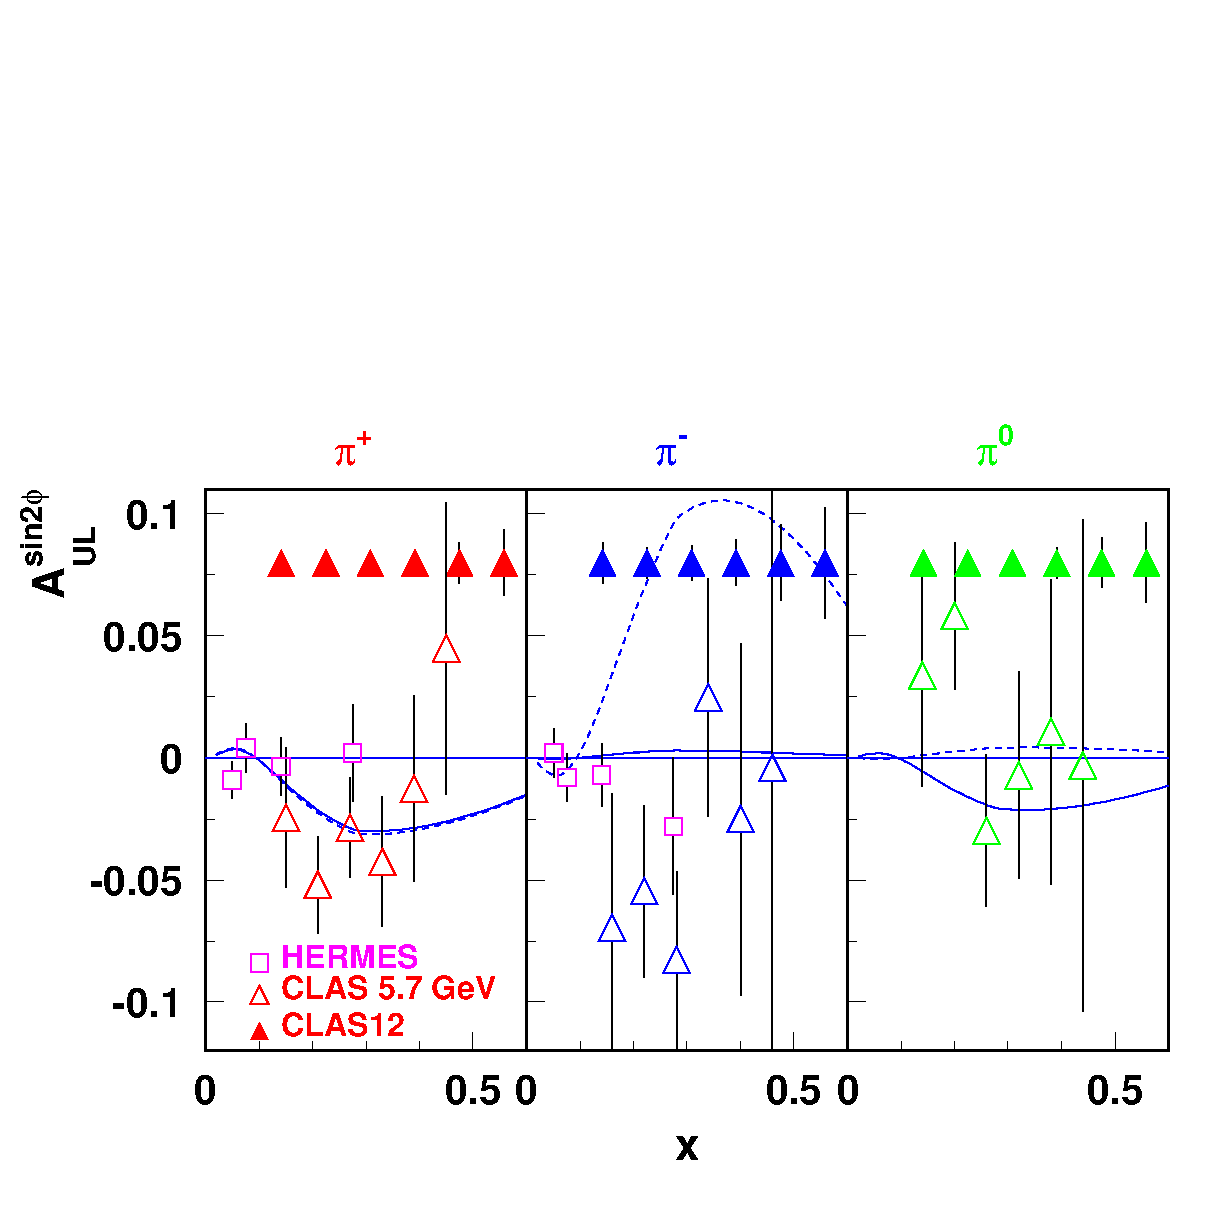
\includegraphics[height=.4\textheight,width=0.45\textwidth]{../sidis/aul11.sin2.eps}
&
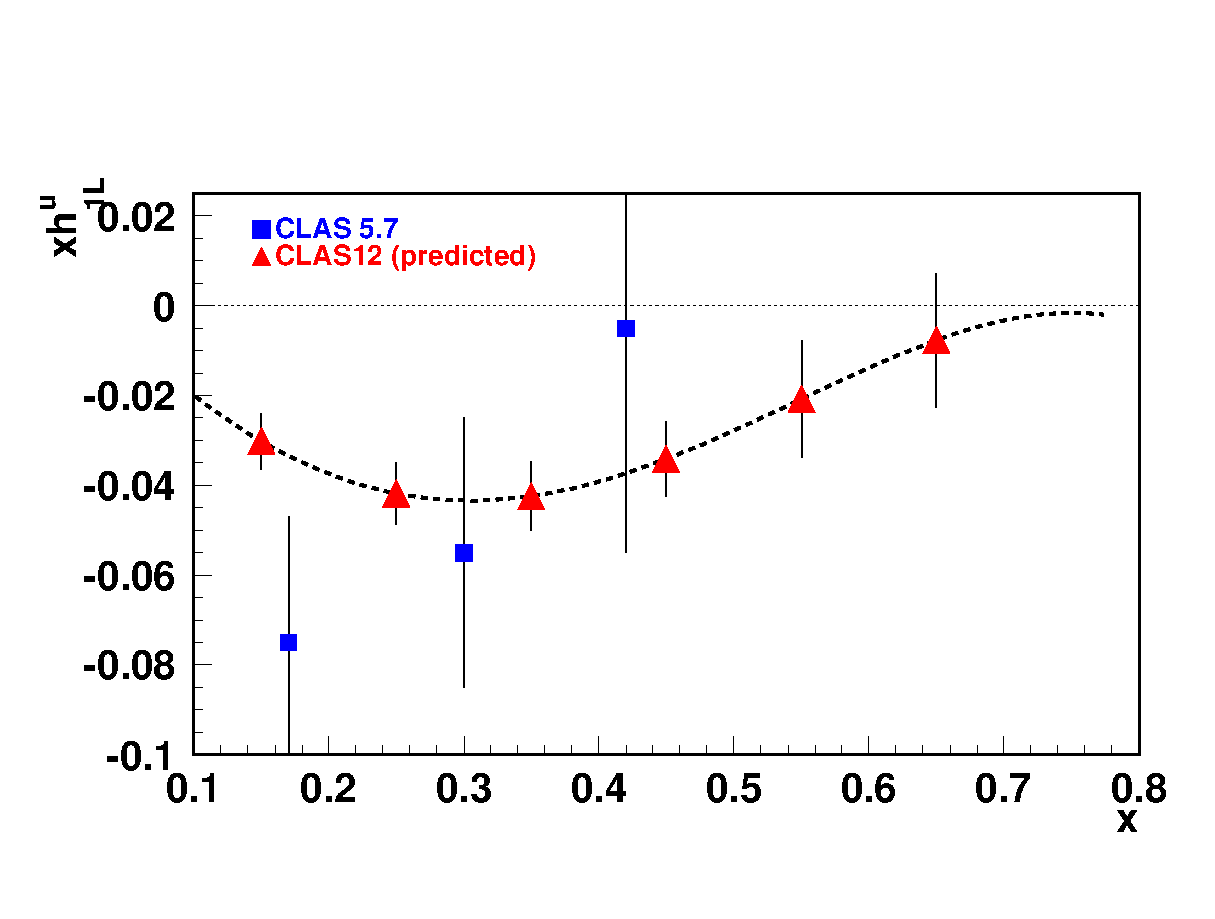
\includegraphics[height=.31\textheight,width=0.45\textwidth]{../sidis/h1lu11.eps}
\\
(a) & (b)
\end{tabular}
\caption{\small{(Left) The projected $x$-dependence of the target SSA at 
11~GeV.  The triangles illustrate the expected statistical accuracy.  The open 
squares and triangles show the existing measurement of the Mulders TMD from 
HERMES and the {\tt CLAS} 5.7~GeV EG1 data sets, respectively.  The curves 
are calculated using Ref.~\cite{Efremov:2004hz}. (Right) Projection for the
Mulders distribution function for the $u$-quark from the $\pi^+$ SSA from 
{\tt CLAS12} (predicted) compared with the {\tt CLAS} EG1 data set at 
5.7~GeV.}}
\label{fig:aul11.sin2}
\end{figure}
%%%%%%%%%%%%%%%%%%%%%%%%%%%%%%%%%%%%%%%%%%%%%%%%%%%%%%%%%%%%%%%%%%%%%%%%%%%%%

Proposed measurements of SSAs in SIDIS will pin down the corresponding TMD 
distribution and will constrain the ratio of favored to unfavored polarized 
fragmentation functions.  The new data will also allow a more precise test of 
the factorization ansatz and the investigation of the $Q^2$ dependence of  
$\sin 2\phi$, $\sin \phi$, and $\cos \phi$ asymmetries. This will enable us 
to study the leading-twist and higher-twist nature of the corresponding 
observables~\cite{Levelt:1994np,Jaffe:1991ra,Kotzinian:1999dy,Afanasev:2003ze,
Yuan:2003gu,Metz:2004je,Collins:2004nx}.

The Boer-Mulders contribution, being leading twist, is expected to survive at 
higher $Q^2$ and that can be tested at the large $Q^2$ accessible with 
{\tt CLAS12}.  At large transverse momentum, {\it i.e.} 
$P_{h\perp}\gg \Lambda_{\rm QCD}$, the transverse-momentum dependence of the 
various factors in the factorization formula~\cite{Ji:2004wu} may be 
calculated from perturbative QCD.  Following the similar arguments in 
Ji-Qiu-Vogelsang-Yuan~\cite{Ji:2006vf}, the $\cos 2\phi$ azimuthal asymmetry 
has the following behavior at $\Lambda_{\rm QCD}\ll P_{h\perp}\ll Q$,

\begin{equation}
\langle \cos 2\phi\rangle|_{P_{h\perp}\gg\Lambda_{\rm QCD}}\propto
\frac{1}{P_{h\perp}^2} \ .
\end{equation}

When the transverse momentum is compatible with the large-scale $Q$, the above 
results will be modified, because the gluon radiation from the pQCD diagram 
will dominate, and contribute to the azimuthal asymmetry not being suppressed 
by any hard scale.  At $Q^2$ values accessible at JLab ($1.0<Q^2<10$~GeV$^2$), 
however, the reduction of the Boer-Mulders asymmetry due to Sudakov form 
factors arising from soft gluon contributions~\cite{Boer:2001he} is not 
expected to be significant.

Measurement of the $P_T$ dependence of the Boer-Mulders-asymmetry (see 
Fig.~\ref{fig:aucos21mx}) will allow for checking of the predictions of a 
unified description of SSA by Ji and collaborators~\cite{Ji:2004wu,Ji:2006vf} 
and for study of the transition from a non-perturbative to a perturbative 
description.  The $\cos 2 \phi$ asymmetry for semi-inclusive deep inelastic 
scattering in the kinematic regions of {\tt CLAS12} is predicted to be 
significant (a few percent on average) and tends to be larger in 
the small-$x$ and large-$z$ region. The preliminary data from {\tt CLAS} at 
6~GeV indeed indicate large azimuthal moments both for $\cos\phi$ and 
$\cos 2\phi$.

%%%%%%%%%%%%%%%%%%%%%%%%%%%%%%%%%%%%%%%%%%%%%%%%%%%%%%%%%%%%%%%%%%%%%%%%%%%%%
\begin{figure}[htbp]
\vspace{6.9cm}
\special{psfile=../sidis/auucos21mxnew.eps hscale=60 vscale=57 hoffset=50 voffset=-5}
\caption{\small{The $\cos2\phi$ moment (Boer-Mulders asymmetry) for pions
as a function of $x$ and $P_T$ for $Q^2>2$~GeV$^2$ (right) with {\tt CLAS12} 
at 11~GeV from 2000~hours of running.  Values are calculated assuming
$H_1^{\perp u\rightarrow \pi^+}=-H_1^{\perp u\rightarrow \pi^-}$.}}
\label{fig:aucos21mx}
\end{figure}
%%%%%%%%%%%%%%%%%%%%%%%%%%%%%%%%%%%%%%%%%%%%%%%%%%%%%%%%%%%%%%%%%%%%%%%%%%%%%

The combined analysis of the future {\tt CLAS12} data on 
$\langle \cos 2 \phi \rangle$ and of the previous ZEUS measurements in the 
high-$Q^2$ domain (where higher-twist effects are negligible) will provide 
information on the Boer-Mulders function, shedding light on the correlations 
between transverse spin and transverse momenta of quarks.  Significantly 
increasing the kinematic coverage at large $Q^2$ and $P_T$, {\tt CLAS12}
(see Fig.~\ref{fig:aucos21mx}) will map the quark TMDs in the valence region
allowing study of the transition from a non-perturbative description at small 
$P_T$ to a perturbative description at large $P_T$.
 
Measured single and double spin asymmetries for all pions in a large range of 
kinematic variables ($x_B$, $Q^2$, $z$, $P_{\perp}$, and $\phi$) combined with 
measurements with unpolarized targets will provide detailed information on the 
flavor and polarization dependence of the transverse momentum distributions of 
quarks in the valence region, and in particular, on the $x_B$, $z$, and 
$P_{\perp}$ dependence of the leading TMD parton distribution functions of $u$ 
and $d$ quarks.  Such measurements across a wide range of $x$, $Q^2$, and $P_T$ 
would allow for detailed tests of QCD dynamics in the valence region 
complementing the information obtained from inclusive DIS.  They would also 
serve as novel tools for exploring nuclear structure in terms of the quark and 
gluon degrees of freedom of QCD.

\section{Summary}

In summary, with upgraded energy and luminosity, {\tt CLAS12} can study 
single- and double-spin asymmetries, involving essentially unexplored 
chiral-odd and time-odd distributions functions, including transversity
\cite{Ralston:1979ys,Jaffe:1991ra}, Sivers~\cite{Sivers:1990fh,Brodsky:2002cx,
Collins:2002kn,Ji:2002aa}, Boer-Mulers~\cite{Boer:1997nt}, and Collins
\cite{Collins:1992kk} functions, providing detailed information on the quark 
transverse momentum and spin correlations~\cite{Collins:1992kk,Kotzinian:1994dv,
Mulders:1995dh,Brodsky:2002rv,Jaffe:2002pj}.

Measurements of semi-inclusive processes combined with inclusive and 
exclusive measurements with an upgraded JLab will allow us to study the quark 
structure of the nucleon with unprecedented detail.  Understanding of 
spin-orbit correlations, together with independent measurements related to the 
spin and orbital angular momentum of the quarks, will help to construct a more 
complete picture of the nucleon in terms of elementary quarks and gluons going 
beyond the simple collinear partonic representation.


\chapter{Properties of QCD from the Nuclear Medium}

\section{Introduction}

While the strong interaction seems to be well described by QCD at high
energies, in the non-perturbative domain it remains largely unsolved
and untested. Further, little is known from experiment about the
space-time characteristics of QCD at any energy scale. Exploration of
the QCD phase diagram for hot, dense matter is a large effort in QCD
physics, and these studies can take advantage of pQCD, however, a
QCD-based description of cold, dense matter still represents a 
formidable challenge. Lattice QCD, in combination with chiral effective 
theory, will partly address the non-perturbative physics and the hot, 
dense matter, but space-time processes and non-zero baryon density are 
still inaccessible via lattice techniques.

New experimental access to a number of properties and consequences of
QCD will become available at 12~GeV. Properties of deconfined quarks,
such as their lifetimes and energy loss, can be extracted. The time
evolution of $q\bar{q}$ pairs can be deduced from studies of color
transparency. The process in which hadrons are formed out of energetic 
quarks can be characterized, both in terms of formation times and 
formation mechanisms. The properties of strongly interacting nucleons 
and their connections to cold, dense matter can be accessed with 
precision over a broad kinematic range, potentially connecting to 
astrophysical systems such as neutron stars. These are exciting 
prospects that will provide profound new insights into the space-time 
characteristics of fundamental QCD processes and the nature of cold 
QCD matter.

\boldmath
\subsection{$p_T$ Broadening and the Lifetime of Deconfined Quarks}
\unboldmath

The confinement of quarks into hadrons is the most important
manifestation of the non-Abelian character of QCD. Achieving a
quantitative understanding of confinement is one of the highest
priority endeavors of nuclear and hadronic physics, and ranks as 
one of the great quests of modern science. The effort to understand
confinement is multi-pronged, typically involving hadron spectroscopy
interpreted through the use of models and lattice calculations, which
aim to characterize the effective potential between quarks. In
addition to the effective potential, another important piece of
confinement is the process of color neutralization, wherein a
deconfined colored quark finds colored partners, such that the
resulting system is a color singlet. Experimental access to the
characteristics of the deconfined quark can be obtained using
semi-inclusive deep inelastic scattering on nuclei in specific
kinematic regions.

In deep inelastic scattering (DIS) kinematics with $x>0.1$, quark-pair 
production by the virtual photon is suppressed~\cite{DDBH} and the target 
quark absorbs all of its energy and momentum. Thus, neglecting the 
intrinsic quark momentum, the initial quark energy is $\nu$ and its 
direction is given by the direction of the virtual photon. The quark 
propagates for some distance until its color is neutralized, at which 
point it is contained in a ``pre-hadron'' that subsequently evolves into 
a fully formed hadron~\cite{KNPH}. In the event that the neutralization 
takes place outside of a nuclear target, the interactions of the struck 
quark with the nuclear medium are limited to partonic-level multiple 
scattering, primarily due to the emission of medium-stimulated gluons
\cite{XGXNW}. This multiple scattering broadens the distribution of 
momentum transverse to the virtual photon direction, which is observable 
by measurement of the final state hadron's $p_T^2$ distribution. 
Subtracting the intrinsic quark $p_T^2$ distribution as measured in 
deuterium yields the basic observable of $p_T$ broadening: 

\begin{equation}
\Delta p_T^2=p_T^2(A)-p_T^2(^2H).
\end{equation}

One property of the deconfined quark that can be accessed is its
lifetime, known as the production time $\tau_p$~\cite{SJBAHM88}. 
This is accessed by studying the dependence of $p_T^2$ on $\nu$ for 
several nuclei. Since $\tau_p$ is time dilated in proportion to $\nu$,
the $\nu$ dependence of $p_T^2$ for a series of nuclei of known
dimensions can be deconvoluted to reliably yield an estimate of
$\tau_p$. While measurements with a 5-GeV electron beam have
demonstrated the feasibility of the method~\cite{EG2,Haf06}, with an 11-GeV 
beam a much wider range in $\nu$ will be accessible. An example of a
measurement of this type is shown in Fig.~\ref{pt2}, where
$\Delta p_T^2$ is shown for three nuclei in a range of $\nu$ from 2 to
9~GeV. 

%%%%%%%%%%%%%%%%%%%%%%%%%%%%%%%%%%%%%%%%%%%%%%%%%%%%%%%%%%%%%%%%%%%%%%%%%%%
\begin{figure}[htbp]
\vspace{7.5cm}
\special{psfile=../nuclear/pt2.ps hscale=60 vscale=60 hoffset=45 voffset=-10} 
\caption{\small{A plot of $\Delta p_T^2$ vs. $\nu$ for three different 
nuclei.  Plateaus are observed in the carbon and iron targets for larger 
values of $\nu$, indicating the production length $\tau_p$ is longer than 
the full thickness of either nucleus, but still less than that of the lead 
nucleus.}}
\label{pt2}
\end{figure}
%%%%%%%%%%%%%%%%%%%%%%%%%%%%%%%%%%%%%%%%%%%%%%%%%%%%%%%%%%%%%%%%%%%%%%%%%%%

A second property of the deconfined quark is the rate of its loss of
energy due to gluon emission. This partonic energy loss has a simple
relationship to $\Delta p_T^2$ under certain simplifying assumptions.
This energy loss can be written as:

\begin{equation}
{dE\over{dx}} \approx \frac{3}{4} \alpha_s \Delta p_T^2.
\end{equation}

\noindent
This energy loss has been estimated previously using the Drell-Yan
reaction~\cite{DY1,DY2}, although theoretical ambiguities have hampered the
extraction.  In addition, energy loss by gluon radiation is the primary 
evidence for the quark-gluon liquid discovered at RHIC~\cite{RHIC} 
through the phenomenon known as jet suppression or mono-jet production
\cite{STAR}. Thus these measurements have important interdisciplinary 
connections. In a simple picture, the energy loss can be estimated
simply from data such as that shown in Fig.~\ref{pt2} from the functional 
form and the known properties of the nucleus.  A picture such as that 
shown in Fig.~\ref{pt2} implies the observation of the novel result that 
the total energy loss is proportional to the square of the distance 
traveled through the medium, a result long predicted~\cite{BDPS}.  This 
implies a coherence behavior in QCD analogous to the QED effect known as 
the Landau-Pomeranchuk-Migdal (LPM) effect, in which electron
bremsstrahlung is suppressed by coherent scattering from multiple
scattering centers~\cite{LPM1,LPM2,Migdal}. 

Models for the energy loss of quarks typically contain a parameter called 
the transport coefficient or jet quenching parameter, $\hat{q}$.  While 
difficult to calculate in lattice QCD, this parameter can be calculated 
for a hot medium~\cite{LRW} using the AdS/CFT correspondence that 
connects nonperturbative phenomena in hot, strongly coupled gauge theories 
onto calculable problems in a dual gravity theory~\cite{ADSCFT1,ADSCFT2,ADSCFT3}.
While this technique cannot be applied to a cold medium, an extrapolation 
procedure such as that employed by Baier {\it et al.}~\cite{BAIER1,BAIER2} could 
potentially extrapolate from hot to cold media. 

\boldmath
\subsection{Color Transparency and the Time Evolution of $q\bar{q}$ Pairs}
\unboldmath

The color transparency (CT) phenomenon illustrates the power of exclusive 
reactions to isolate simple elementary quark configurations.  For a hard 
exclusive reaction, such as vector meson electroproduction on the nucleon, 
the scattering amplitude at large momentum transfer is suppressed by 
powers of $Q^2$ if the hadron contains more than the minimal number of 
constituents.  This is derived from the QCD-based quark counting rules. 
Therefore, the hadron containing valence quarks only, participates in the 
scattering.  Moreover, each quark, connected to another one by hard gluon 
exchange carrying momentum of order $Q$, should be found within a distance 
of order $1/Q$. Therefore, at large $Q^2$ one selects a very special 
configuration of the hadron wave function where all connected quarks are 
close together, forming a small size color neutral configuration called 
a Point Like Configuration (PLC).  Such an object is unable to emit or 
absorb soft gluons.  Therefore, its strong interaction with the other 
nucleons becomes significantly reduced, and then the nuclear medium 
becomes more transparent.  The nucleus offers a unique laboratory to study 
quark dynamics.  Indeed, the nucleus can be used as a revealing medium of 
the evolution in time of elementary configurations in the hadron wave 
function.  The time necessary for a quark to cross distances typical of 
the confined systems is of the order of 1~fm.  By taking into account the 
relativistic time dilation factor, the characteristic time scale 
corresponds to length scales on the order of a few fm.  The only medium 
available at this scale is the nucleus, offering to us a new generation of 
experiments where the nucleus functions as bubble chamber!

Experimentally, we would like to understand this spectacular phenomenon by 
studying the hadron attenuation as it propagates through the nuclear 
medium.  These measurements will allow us to not only access the special 
configuration of the hadron wave function, but also to study how this 
configuration dresses with time to form the fully complex asymptotic wave 
function of the hadron.  This puts us in the heart of the dynamics of 
confinement.  Furthermore, the onset of CT is related to the onset of 
factorization, which is an important requirement for accessing Generalized 
Parton Distributions (GPDs) in deep exclusive meson production. The 
$\rho^0$ meson is our hadron of choice because it offers many advantages. 
It is believed that the onset of CT is expected at lower $Q^2$ in the 
($q\bar{q}$) system than in the ($qqq$) system, as it is much more probable 
to produce a small-size system of two quarks than one of three quarks
\cite{Blat}.  In addition, the $\rho^0$ is a vector meson similar to 
the virtual photon. Therefore its production mechanism is fairly well 
understood because the virtual photon fluctuates into a ($q\bar{q}$) pair 
which then materializes into the $\rho^0$ meson. The size of the 
produced ($q\bar{q}$) can be directly connected to the virtuality of the 
photon. Therefore, smaller sizes can be reached at larger $Q^2$.

More than two decades of experimental investigations have lead to only 
one clear signal of CT at high energies.  It was observed in experiment 
E791~\cite{Aita} at Fermilab.  The $A$-dependence of the diffractive 
dissociation into di-jets of 500~GeV pions scattering coherently from 
carbon and platinum targets was measured.  It was found that the cross 
section can be parameterized as $\sigma = \sigma_{0} A^{\alpha}$, with 
$\alpha$ = 1.6.  This result is quite consistent with theoretical 
calculations~\cite{Bert1,Bert2,Bert3} including CT and obviously 
inconsistent with a cross section proportional to $A^{2/3}$, which is 
typical of inclusive pion-nucleus interactions.  At moderate energies, 
the situation is more complicated.  No evidence of CT was found in 
quasi-free $A(e,e'p)$ reactions~\cite{eep1,eep2,eep3,eep4} even for $Q^2$ 
values as large as 8~GeV$^2$.  While the outcome of quasielastic $(p,2p)$ 
scattering from nuclei~\cite{p2p1,p2p2,p2p3} 
was very controversial due to the fact that the results do not support a 
monotonic increase in transparency with $Q^2$ as predicted by CT, the 
transparency increases for $Q^2$ from 3 to 8~GeV$^2$, but then decreases 
for higher $Q^2$, up to 11~GeV$^2$.  This subsequent decrease was 
explained as a consequence of soft processes that interfere with 
perturbative QCD in free $pp$ scattering but which are suppressed in the 
nuclear medium~\cite{ral}.  Other measurements studied the attenuation 
of the $\rho^0$ vector meson in the nuclear medium via exclusive $\rho^0$ 
lepto-production off nuclei.  The results from the two measurements
\cite{meso1,meso2} are very suggestive of a CT signal, but they are 
statistically limited.

The exclusive, diffractive, incoherent electroproduction of vector mesons 
off nuclei has been suggested~\cite{kop02} as a sensitive way to detect 
CT.  In the laboratory frame, the photon fluctuation can propagate over 
a distance $l_c$ known as the coherence length.  The coherence length can 
be estimated relying on the uncertainty principle and Lorentz time dilation 
as $l_c = 2 \nu/(Q^2 + M^2_{q\bar{q}})$, where $\nu$ is the energy of the 
virtual photon in the laboratory frame, (-$Q^2$) is its squared mass, and 
$M_{q\bar{q}}$ is the mass of the ($q\bar{q}$) pair.  In the case of 
exclusive $\rho^0$ electroproduction, the mass of the ($q\bar{q}$) is 
dominated by the $\rho^0$ mass.  The produced small-size, colorless 
hadronic system will then propagate through the nuclear medium with 
reduced attenuation because its cross section is proportional to its size. 
The effect of the nuclear medium on the particles in the initial and final 
states can be characterized by the nuclear transparency $T_A$.  $T_A$ is 
defined as the ratio of the measured exclusive cross section to the cross 
section in the absence of initial and final state interactions.  It can be 
measured by taking the ratio of the nuclear per-nucleon ($\sigma_A/A$) to 
free nucleon ($\sigma_N$) cross sections:

\begin{equation}
T_A = \frac{\sigma_A}{A\sigma_N}.
\end{equation}

The signal of CT would be an increase of the nuclear transparency as 
$Q^2$ increases.  It was shown by the HERMES collaboration~\cite{acker} 
that the nuclear transparency increases when $l_c$ varies from long to 
short compared to the size of the nucleus.  This is due to the fact that 
the nuclear medium seen by the ($q\bar{q}$) fluctuation becomes shorter. 
Thus the ($q\bar{q}$) pair interacts less.  This situation occurs when 
$Q^2$ increases at fixed $\nu$.  This so-called coherence length effect 
(CL) can mimic the CT signal.  Therefore one should keep $l_c$ fixed while 
measuring the $Q^2$ dependence of the nuclear transparency.

{\tt CLAS12} is the ideal detector for such measurements.  It offers large 
acceptance, good particle identification, and high luminosity. Using 
an 11-GeV electron beam, one can extend the $Q^2$ region up to
5.5~GeV$^2$. An indication of the quality of the data that can be
obtained is shown in Fig.~\ref{res}. 
The nuclear transparency for several targets (C, Fe, and Sn) could be 
measured.  This is important in order to study the formation time of the 
hadron as it propagates through different nuclear sizes.  These 
measurements would also be a natural extension of a previous {\tt CLAS} 
experiment~\cite{koko}, where the preliminary results indicate a clear 
evidence of a CT signal despite the limited $Q^2$ range to 2~GeV$^2$.

%%%%%%%%%%%%%%%%%%%%%%%%%%%%%%%%%%%%%%%%%%%%%%%%%%%%%%%%%%%%%%%%%%%%%%%
\begin{figure}[htbp]
\vspace{9.0cm}
\special{psfile=../nuclear/tr_err_fe.eps hscale=70 vscale=65 hoffset=40 voffset=0}
\caption{\small{A plot indicating the expected error bars for the 11-GeV 
measurements of nuclear transparency for $\rho_0$ production on Fe from 
incoherent $\rho$ electroproduction (12 days of beam time), and the 
predictions of Ref.~\cite{kop02}.}}
\label{res}
\end{figure}
%%%%%%%%%%%%%%%%%%%%%%%%%%%%%%%%%%%%%%%%%%%%%%%%%%%%%%%%%%%%%%%%%%%%%%%

\section{Hadron Attenuation and the Formation Time of Color Fields}

In the preceding discussion, the focus was on the kinematics in which the 
color of the quark is neutralized outside the nucleus.  In those kinematics 
one learns about the properties of the propagating quark through its 
partonic-level multiple scattering in the medium. In this section the focus 
is on the case when the color neutralization happens within the nuclear 
medium, creating a color singlet object referred to as a pre-hadron. The 
pre-hadron evolves to a full hadron over a period of time $\tau_f$, the 
formation time.  The pre-hadron and the final hadron can both interact with 
the nuclear medium and the most probable interaction is a highly inelastic 
reaction. Relative to the same kinematics on deuterium, in a heavy nucleus 
these interactions move hadron flux at high energies to lower energies (or
lower $z$) and higher multiplicities. This is referred to as hadron 
attenuation. It is quantitatively measured by the hadronic multiplicity 
ratio $R_M^h$:
    
\begin{equation}
R_M^h = \frac{(N_h^{DIS,A})/(N_e^{DIS,A})}
{(N_h^{DIS,^2H})/(N_e^{DIS,^2H})},
\end{equation}

\noindent
where $N_h^{DIS,A}$ is the number of hadrons of species $h$ produced
in DIS kinematics on nucleus $A$, $N_e^{DIS,A}$ is the number of DIS
electrons from nucleus $A$, and the denominator refers to the same
quantities for deuterium $^2H$~\cite{HERMES}. $R_M^h$ may in principle
depend on a number of kinematic variables such as $Q^2$, $\nu$, $z$,
$p_T$, and $\phi$. Isolating the multi-variable dependence of $R_M^h$
is a powerful discriminator between models based on different physical
pictures. At the current time, two different physical pictures
dominate model descriptions. The first~\cite{WANG,ARLEO} assumes that 
hadronization takes place outside the nucleus. The second
\cite{KNPH,MOSEL} assumes that hadronization can take place inside the 
nucleus, and cite the interaction of the pre-hadron as the main cause of 
the attenuation.  Both approaches provide adequate descriptions of the 
HERMES data, which is statistics limited to one or at most two dimensional
analyses. A full multi-dimensional analysis spanning a wide kinematic
range is feasible with {\tt CLAS12}, and such an analysis will be certain 
to strongly constrain theoretical descriptions. In addition to spanning a
range of kinematic variables, it is feasible to measure a wide range
of hadron masses with varied flavor content, as may be seen in
Table~\ref{table:hadron_list}, which lists hadrons with $c\tau$ greater
than nuclear dimensions for which measurements with {\tt CLAS12} are
feasible. With a dataset of this quality and breadth, a comprehensive
program to extract hadron formation lengths is practical to carry
out. Such a program will yield insights into the systematic behavior
of how hadrons form, a heretofore unknown sector of nonperturbative
QCD in the spacetime domain.  

%%%%%%%%%%%%%%%%%%%%%%%%%%%%%%%%%%%%%%%%%%%%%%%%%%%%%%%%%%%%%%%%%%%%%%%
\begin{table}[htbp]
\begin{center}
\begin{tabular}{||c|c|c|c|c|c||} \hline \hline
hadron & $c\tau$ & mass & flavor  & detection & Production rate\\
       &         &(GeV) & content &  channel &  per 1k DIS events\\ \hline \hline
$\pi^0$ & 25 nm & 0.13 & $u\bar{u}d\bar{d}$ & $\gamma\gamma$ & 1100 \\ \hline
$\pi^+$ & 7.8 m & 0.14 &   $u\bar{d}$ & direct & 1000 \\ \hline
$\pi^-$ & 7.8 m & 0.14 &   $d\bar{u}$  & direct & 1000 \\ \hline
$\eta$ & 0.17 nm & 0.55 & $u\bar{u}d\bar{d}s\bar{s}$&$\gamma\gamma$ & 120 \\ \hline
$\omega$ & 23 fm & 0.78 &  $u\bar{u}d\bar{d}s\bar{s}$ & $\pi^+\pi^-\pi^0$ & 170 \\ \hline
$\eta'$ & 0.98 pm & 0.96 &  $u\bar{u}d\bar{d}s\bar{s}$ & $\pi^+\pi^-\eta$ & 27 \\ \hline
$\phi$ & 44 fm & 1.0 &  $u\bar{u}d\bar{d}s\bar{s}$ & $K^+K^-$ & 0.8 \\ \hline
$f1$ & 8 fm & 1.3 &  $u\bar{u}d\bar{d}s\bar{s}$ & $\pi\pi\pi\pi$ & - \\ \hline
$K^+$ & 3.7 m & 0.49 &  $u\bar{s}$ & direct & 75 \\ \hline
$K^-$ & 3.7 m & 0.49 &  $\bar{u}s$ & direct & 25 \\ \hline
$K^0$ & 27 mm & 0.50 &  $d\bar{s}$ & $\pi^+\pi^-$ & 42 \\ \hline
$p$ & stable & 0.94 &  $ud$ & direct & 530 \\ \hline
$\bar{p}$ & stable & 0.94 &  $\bar{u}\bar{d}$ & direct & 3 \\ \hline
$\Lambda$ & 79 mm & 1.1 &  $uds$ & $p\pi^-$ & 72 \\ \hline
$\Lambda(1520)$ & 13 fm & 1.5 &  $uds$ & $p\pi^-$ & - \\ \hline
$\Sigma^+$ & 24 mm & 1.2 &  $us$ & $p\pi^0$ & 6 \\ \hline
$\Sigma^0$ & 22 pm & 1.2 &  $uds$ & $\Lambda\gamma$ & 11 \\ \hline
$\Xi^0$ & 87 mm & 1.3 &  $us$ & $\Lambda\pi^0$ & 0.6 \\ \hline
$\Xi^-$ & 49 mm & 1.3 &  $ds$ & $\Lambda\pi^-$ & 0.9 \\ \hline \hline	
\end{tabular}
\end{center}
\caption{\small{Final-state hadrons potentially accessible for formation 
length and transverse momentum broadening studies in {\tt CLAS12}. The 
rate estimates were obtained from the LEPTO event generator for an 11-GeV 
incident electron beam. (The criteria for selection of these particles 
was that $c\tau$ should be larger than the nuclear dimensions, and their 
decay channels should be measurable by {\tt CLAS12}.)}}
\label{table:hadron_list}  
\end{table}
%%%%%%%%%%%%%%%%%%%%%%%%%%%%%%%%%%%%%%%%%%%%%%%%%%%%%%%%%%%%%%%%%%%%%%%

\boldmath
\subsection{$D(e,e'p_s)$ and the Quark Structure of Neutrons in a Cold
Dense Medium}
\unboldmath

For a complete understanding of QCD at hadronic scales, we need to 
learn more about the interplay between the internal (quark) structure 
of nucleons and the interaction between two nucleons. In particular, it 
is of high interest whether nucleons in close proximity to each other
(effectively at non-equilibrium high density) change their internal 
structure or perhaps even lose their separate identity to fuse into a 
``six quark cluster''~\cite{Carlson}.  Some less dramatic modifications 
of the nucleon structure that have been proposed include off-shell 
effects~\cite{MT}, $Q^2$ rescaling effects, and the suppression of
small-size configurations (PLCs) in the nucleon wave function
\cite{FS81,FS85}.  Deuterium is the optimal system to study such 
``tightly bound pairs'', since there are no additional nucleons 
interacting with the pair under study and the pair is at rest in the lab, 
with completely defined kinematics.  While the probability for a small 
inter-nucleon distance configuration in deuterium is rather small 
compared to heavier nuclei, such configurations can be ``tagged'' by the 
emission of a fast proton in the backward hemisphere relative to the 
momentum transfer vector.  We therefore propose to measure the reaction 
$D(e,e'p_b)X$ with coincident detection of the scattered electron in the 
forward part of {\tt CLAS12} and the fast (above 300~MeV) backwards 
proton in the central detector.

In the simple spectator picture, the backwards-moving proton does not 
participate in the scattering process and can serve as a tag of the 
initial state momenta of both nucleons.  By measuring the momentum of
this backward proton, we can correct the observed electron kinematics 
for the initial motion of the unobserved struck neutron and extract the 
modified neutron structure function $F_2^{n(eff)}(x, Q^2, p^2)$.
The emphasis here is not on nearly on--shell neutrons, but rather on
the opposite kinematic extreme of fast--moving neutrons, where off-shell
effects and other internal structure changes are much more pronounced.
We can extract the dependence of the structure function 
$F_2^{n(eff)}(x, Q^2, p^2)$ at fixed $x$ and $Q^2$ on the spectator
momentum $p$ in the range from about 70~MeV to 700~MeV.  We will 
simultaneously cover a large range in $x$ and $Q^2$, allowing us to make 
detailed comparisons with the different models mentioned above, including 
the rather striking change in the shape of the structure function $F_2$ 
predicted for a non-trivial six quark configuration~\cite{Carlson}.

For the proposed experiment, we will use {\tt CLAS12} in the standard
configuration, with a liquid-deuterium target and the fully 
instrumented central detector to tag the backward proton. We estimated 
the expected number of counts for a 20-day run with full luminosity
(10$^{35}$ cm$^{-2}$s$^{-1}$). The results are shown in Fig.~\ref{deeps}
as a function of the ``ordinary'' Bjorken variable $x = Q^2/2m\nu$
in the lab and for several bins in the light cone fraction $\alpha$ of
the backward proton. One can clearly see the kinematic shift due to the 
motion of the struck neutron, which we can fully correct using the proton 
kinematics.  We clearly will have good statistics for a large range in 
$x$ and in $\alpha$ (the highest bin corresponds to more than
600~MeV momentum opposite to the direction of the $q$ vector),
drastically extending the kinematic coverage and statistical precision
of the existing data from the analog experiment at 6~GeV (E94-102)
\cite{e94102}.

%%%%%%%%%%%%%%%%%%%%%%%%%%%%%%%%%%%%%%%%%%%%%%%%%%%%%%%%%%%%%%%%%%%%%%%
\begin{figure}[htbp]
\vspace{8.6cm}
\special{psfile=../nuclear/deeps.eps hscale=65 vscale=55 hoffset=35 voffset=-15}
\caption{\small{Kinematic coverage in Bjorken--$x$ and proton light-cone 
fraction $\alpha_S$ for the proposed experiment. The count rates have
been estimated for a 20-day run with the standard {\tt CLAS12} 
configuration.}}
\label{deeps}
\end{figure}
%%%%%%%%%%%%%%%%%%%%%%%%%%%%%%%%%%%%%%%%%%%%%%%%%%%%%%%%%%%%%%%%%%%%%%%

\section{$x>1$ and the Properties of Cold Dense Matter} 

Measurements with $x>1$ have been demonstrated to provide insight into
the properties of nucleon-nucleon correlations~\cite{EGIYAN,ARRINGTON}. 
With {\tt CLAS12}, the combination of increased luminosity and large 
acceptance promises to permit investigation of the hadronic final states 
associated with $x>>1$, which means that the properties of cold nuclear 
matter fluctuating ephemerally to conditions of high density can be 
accessed experimentally.  Together with theoretical extrapolations to 
equilibrium conditions, one can hope to explore such exotica as stable 
strange matter as an equilibrium component of neutron stars. A
possible experimental avenue to explore these ideas is to measure
strangeness production on a series of nuclei in $x>1$ kinematics. A
significant enhancement in kaon production increasing with $x$ may be
a signature that can be connected to equilibrium conditions at high
nuclear density which have a persistent strangeness component. These
studies complement investigations in heavy-ion reactions~\cite{GSI}
where kaon yields have recently been shown to be consistent with
thermal production in high-density nuclear matter. These exclusive or
semi-inclusive studies with $x>1$ are the natural next step following
the inclusive experiments to date. 

\subsection{The Polarized EMC Effect and the Quark Structure of Nuclei}

The well known ``EMC effect'', which shows a modification of the
$F_2$ structure function in nuclei relative to the proton, has been
a puzzle for over two decades.  Nearly 1000 papers have been written
on the subject to try to explain the EMC effect and its associated
phenomena.  The best models generally use a modification of the nucleon 
structure within the nuclear medium to explain the effect.  It is
known from lattice QCD that the region surrounding a baryon or a meson
has a suppressed chiral condensate, and it is reasonable to infer that
the nuclear medium continues this pattern.  In a quantum field theory
picture of the nucleus, the structure of bound baryons is dominantly
affected by the scalar field of the nucleus, which essentially
polarizes the nucleon and modifies its structure, particularly that of
the lower component of the relativistic wave function.  Calculations of
the polarized EMC effect indicate it is approximately twice as big as
the unpolarized effect~\cite{CLOET}.  A plot indicating the achievable
uncertainties is shown in Fig.~\ref{p_emc}.

%%%%%%%%%%%%%%%%%%%%%%%%%%%%%%%%%%%%%%%%%%%%%%%%%%%%%%%%%%%%%%%%%%%%%%%
\begin{figure}[htbp]
\vspace{6.5cm}
\special{psfile=../nuclear/REMC.eps hscale=60 vscale=60 hoffset=70 voffset=-15}
\caption{\small{A plot of the polarized EMC effect for an 11-GeV beam, 40\% 
target polarization, 80\% beam polarization, and 70 PAC days measured in 
{\tt CLAS12}. The two curves are for the two dominant structure function 
multipoles for this ($J^{\pi}=3/2^-$) nucleus; the solid line is for $K=1$ 
and the dashed line is for $M=J$.}}
\label{p_emc}
\end{figure}
%%%%%%%%%%%%%%%%%%%%%%%%%%%%%%%%%%%%%%%%%%%%%%%%%%%%%%%%%%%%%%%%%%%%%%%

\chapter{Spectroscopy}

\section{Introduction}

Spectroscopy of hadrons (mesons and baryons) is one of the key tools
for studying the theory of strong interactions, Quantum Chromodynamics 
(QCD), in the non-perturbative ({\it i.e.} confinement) regime. Hadron 
spectroscopy has been an essential component of the physics program with 
{\tt CLAS}~\cite{clas3pi,clas-d,clas-p,Tho01,McN04,Pri04,Guo07,5st}. To 
date, a large amount of experimental data on electromagnetic production of 
hadrons has been collected by {\tt CLAS}. However, more data will be 
necessary to guide improvements in hadronic phenomenology and to compare 
with lattice QCD calculations.

The majority of the data obtained so far with {\tt CLAS} is restricted to
the lowest mass states formed with the lightest quarks, up, down, and 
strange. A complete picture of QCD in the strong-coupling (non-perturbative) 
regime requires extension of hadron spectroscopy studies to higher masses 
and/or higher transferred momenta. Fulfillment of this task requires 
upgrading the electron beam energy to about 12~GeV, along with the necessary 
upgrade of the detector package, with a large-acceptance spectrometer being 
an obvious choice for studies of multi-particle final states.

The key experiments in hadron spectroscopy that we plan for the upgraded 
{\tt CLAS} detector ({\tt CLAS12}) will study reactions produced by both 
quasi-real and virtual photons.  They include:

\begin{itemize}

\item Studies of high-mass mesonic states (consisting of ordinary mesons, 
hybrids, and mesons with exotic $J^{PC}$) using H$_2$ and light nuclear 
targets;

\item Higher mass baryon production, {\it e.g.} $\Sigma$ and $\Xi$ baryons; 

\end{itemize}

Along with traditional bremsstrahlung photon beams, we are planning to 
use quasi-real photons produced when electrons are scattered at very 
forward angles ({\it i.e.} scattering angles $<$1.5$^\circ$). We plan to 
use a small-angle forward electron tagger in coincidence with the detection 
of multi-particle final states with the {\tt CLAS12} detector to study 
electroproduction at $Q^2$ values of $<10^{-2}$~GeV$^2$.  
{\it Electroproduction at these very small values of $Q^2$ using 
unpolarized electrons is equivalent to photoproduction using partially 
linearly polarized photons}~\cite{Dom69}.

The physics program using the very small-angle electron scattering
facility will take advantage of polarized photons and relatively high
photon fluxes. The use of high precision, high intensity electron beams 
will allow us to achieve the required luminosities on very thin targets 
({\it i.e.} gas targets) without jeopardizing the signal to accidental 
ratio. In turn, this will allow detection of low-energy recoils ({\it e.g.} 
coherent scattering experiments) and spectators ({\it e.g.} scattering 
off of the neutron in the deuteron). High-flux, linearly polarized
photon beams, together with the use of the nearly $4\pi$ coverage for 
hadronic final states of {\tt CLAS12}, will allow the study of hadron 
spectroscopy in a competitive and complementary experimental environment 
to the already planned {\tt GlueX} coherent bremsstrahlung production 
experiment in Hall D.

\section{Physics Motivation}

Perhaps the most fundamental question of interest to hadron physicists
is that of understanding the mechanism of confinement. It has been more
than thirty years since QCD was postulated as the theory of strong
interactions.  While much progress has been made in understanding
perturbative phenomena, the non-perturbative regime, the regime of
hadrons, their excitations, and their couplings, has remained largely
impervious to our varied assaults.  Only recently, with improvements 
to calculations of lattice QCD, has it become possible to make 
predictions of the spectrum of hadrons~\cite{morningstar,mathur}
directly from QCD, based on very few parameters (such as the bare quark 
masses). New experimental efforts to determine the hadron spectra are 
timely and are important for theoretical progress in non-perturbative QCD.

In order for this lattice effort to make significant progress in addressing 
confinement, and in order for this investment to pay off, lattice 
calculations for the masses and couplings of baryons and mesons must be 
compared with information extracted from precision experiments. Lattice 
QCD is not only capable of studying masses of bound systems of quarks 
and gluons, but it can also give insight into a space-time picture of 
electromagnetic interactions of these systems through studying the $Q^2$ 
dependence of electro-excitation form factors. We can have confidence that 
lattice calculations are indeed simulating QCD only when it successfully
reproduces a wide range of hadron properties. Some of the precision
experiments needed have been, and are being, carried out at Jefferson
Lab, and at other facilities around the world.

While mesons and baryons may be viewed differently, their phenomenology 
reflects common aspects of strong interaction dynamics. Searching for 
mesons with exotic quantum numbers gives us an opportunity to capture 
gluons as constituent particles that have their own identity, along with 
quarks, in forming hadronic bound states. On the other hand, considering 
interactions between three quarks in a baryon, one finds that the presence 
of meson-type quark correlations may be crucial in describing baryon 
properties, reflecting fundamental features of the QCD vacuum. In addition, 
multi-quark configurations in baryons are possible.

A number of legitimate questions about why this research is important
might be asked. For instance, some may question the need for more
experiments in hadron spectroscopy, since many experiments have already
addressed some of the issues discussed here. However, the experimental
coverage is incomplete. Many individual experiments have been carried out
with the aim of addressing single aspects of hadron phenomenology. Like a
map drawn by many hands, the picture of hadrons that has emerged is
incomplete in some areas, and inconsistent in others.  The goal of further
experimentation in this area is compelling: to continue our efforts to
arrive, as far as possible, at a clear, complete, and consistent
description of hadrons and their properties.

In order to understand the dynamics of QCD in the confinement region, a 
systematic study of many states, including their couplings to other states, 
is needed. Many of the current experiments at JLab, in combination with a 
systematic analysis effort, will have (in principle) information primarily 
on non-strange baryons, the nucleons and the Deltas. This information is 
not sufficient for us to arrive at a complete and consistent picture of 
the dynamics of QCD in the confinement region. Information on hyperons is
a crucial element needed for constructing such a picture. For instance,
the SU(3) singlet $\Lambda$s play key roles in identifying the states of
the 70-plets and the 20-plets.  At present, only one paper from {\tt CLAS} 
on the excited $\Lambda^*$s~\cite{barrow} has been published, and 
this study was statistically limited by the low production cross 
sections at the currently available beam energies.  Other studies of the 
excited hyperon states are in progress at {\tt CLAS} and further work can 
be done with the availability of higher energies. 

Some information on hyperons can be extracted from ongoing experiments,
but the kinematic reach of the current JLab accelerator at present does 
not allow the kind of systematic study that is essential.  The higher 
energies provided by the upgraded facility will allow for more detailed 
analysis of the spectrum and interactions of the hyperons, through 
processes like $\gamma N \to K \bar{K} N$ and $\gamma N \to KK\Xi$. 

The proposed {\tt CLAS12} experimental program is in step with current 
developments in hadronic phenomenology and lattice QCD, where the main 
thrust is a comprehensive study of the spectrum of conventional hadrons,
along with hybrid and exotic mesons and baryons. 

\section{Meson Spectroscopy}

A complete mapping of meson resonances in the mass region of 1 to 3~GeV
will be particularly important for a better understanding of the QCD 
confinement mechanism. QCD predicts the existence of several new types 
of states beyond the naive quark model, {\it e.g.}: glueballs, hybrids, 
and multi-quark $q\bar{q} q\bar{q}$ states~\cite{Is85,Ko85}.  Gluons play 
a central role in strongly interacting matter -- quark confinement is due 
to gluonic forces. The clearest most fundamental experimental signature for 
the presence of dynamics of gluon degrees of freedom is the spectrum of 
gluonic excitations of hadrons. Gluonic excitations of mesons with 
``exotic'' quantum numbers, {\it i.e.} quantum numbers not accessible 
to the $q\bar{q}$ system, would be the most direct evidence for these
states. Determining the properties of such states would shed light on
the underlying dynamics of quark confinement.

The identification of these states has been difficult, as high-mass
resonances are generally broad and overlapping, and often have similar
quantum numbers (mixing). Photoproduction cross sections are small, so
statistics have been limited. Ideally, for a complete mapping of the
mesons in this mass region, we will need to study each resonance
through as many decay channels and production mechanisms as possible
in order to disentangle mixing. To determine meson quantum numbers, we
use partial wave analysis (PWA) (in a broad sense, fits to the angular
distributions of final states). A complete PWA requires high event
statistics, as well as high resolution and geometrical acceptance of
the detector. Meson spectroscopy at {\tt CLAS12}, using the low-$Q^2$ 
tagger, will fulfill many of these stipulations.

\subsection{Coherent Photoproduction on Light Nuclei}
\label{he4}

In the electromagnetic production of $t$-channel meson resonances
at moderate energies, the main physics background arises from
associated production of baryon resonances that decay into the same
final state particles.  Often these particles in both production reactions
occupy the same phase space, and therefore, it becomes impossible to
separate them using kinematic cuts. The contribution of baryon
resonances to the final state makes PWA analysis rather complicated. The 
production of meson resonances coherently on nuclear targets, when the
recoiling nucleus remains intact, is a {\it clean} way to eliminate
baryon resonances. A particular case of such processes is coherent 
production off of light nuclei, {\it e.g.} $^3$H, $^3$He, and $^4$He. For
these reactions, the recoiling nuclei can be detected in order to ensure 
that they remain intact.

We propose a program to study charged and neutral meson resonances in
the coherent production reactions on light nuclei,
$\gamma^* \,^3{\rm H}  \to \,^3{\rm He}\,M^-$, 
$\gamma^* \,^3{\rm He} \to \,^3{\rm H} \,M^+$, and
$\gamma^* \,^4{\rm He} \to \,^4{\rm He}\,M^0$, 
using the {\tt CLAS12} detector and the 12-GeV electron beam. 
{\it The key feature of these measurements is the detection of the 
recoiling nuclei}.

For meson masses from 1 to 3~GeV, the minimum transferred momentum, 
$t_{min}$, at beam energies up to 10~GeV, ranges from 0.02 to 0.2~GeV$^2$. 
At these transferred momenta, reduction of yields due to the nuclear form 
factor is expected to be only a factor of a few, while the energy obtained 
by the recoiling nucleus, 5 to 30~MeV for $^3$H, $^3$He, and $^4$He, will 
be enough to detect them using thin gas targets. Such experiments can 
only be conducted with high-intensity electron beams, where the low density 
of the target can be compensated for by a high flux of quasi-real photons. 
High precision electron beams, with sub-millimeter cross sections, will 
allow us to use a small diameter target cell, consequently to have thin 
windows at high pressure, a critical component for the detection of 
low-energy recoiling particles.  {\it Electron scattering at very small 
angles is a unique technique for experiments on thin targets.}

Besides the elimination of baryon resonances, coherent production on
nuclei has other advantages as well. In many cases it imposes constraints
on the allowed helicity states of the produced meson, and on the possible
exchange particles. These will significantly aid the PWA.

Examples of such reactions include coherent production of $\pi \eta$ and
$\pi \eta'$ final states on $^4$He~\cite{stephe4}.  The attractive
feature of these final states is that in the $P$-wave they have
exotic quantum numbers, $J^{PC}=1^{-+}$. Photoproduction of $\pi \eta$
and $\pi \eta'$ on the nucleon proceeds only via C-odd $\rho$ or
$\omega$ exchanges. Since $^4$He has isospin 0, only $\omega$ exchange
is allowed, and as $^4$He has spin 0, the helicity of the final state
(at small angles) should be equal to the helicity of the incoming photon 
(SCHC).

\subsection{Electroproduction on the Proton at Very Small Q$^2$} 

The general idea of PWA is to parameterize the intensity distribution
in the space of quantum numbers available to the observed final
states. The intensity distribution is written as a sum of interfering
and non-interfering amplitudes (partial waves). A maximum likelihood
fit is done to the intensity distribution by a set of given partial
waves and reasonable assumptions of the production mechanism.  The
goodness of the fit is related to the statistics (number of events per
binned data), the rank of the production matrix, and the number of
parameters to be fitted. The fit could then be improved by using
higher statistics or (equivalently) by reducing the rank of the fit by
having more information about the production mechanism.

The knowledge of photon polarization simplifies the PWA by giving
direct information on the production mechanism, and therefore, reducing
the rank of the fit. In electroproduction at very low $Q^2$, we will
be able to measure, on an event-by-event basis, the linear polarization
of the photons.

Spectroscopy studies of mesons have started with {\tt CLAS} at lower 
energies~\cite{Ad01}.  Preliminary results of these experiments show the 
viability of such studies using the current {\tt CLAS} configuration, 
where PWA of simple final states ($\pi\pi\pi$) has already been carried 
out successfully.  However, with the limited acceptance of the present 
{\tt CLAS} and only circular polarization of the electron beam, there are 
many analysis ambiguities created by the assumptions on the production 
mechanism and the baryon backgrounds. These ambiguities will be mostly 
resolved when using linearly polarized, high-energy (greater than 8~GeV) 
photons, and larger acceptances. At higher energies we will be able to map 
out the mesons in the interesting 1 to 3~GeV mass range and, most 
importantly, to better kinematically differentiate mesons from baryons. More
specifically, we plan to study mesons decaying into multiple final states 
({\it e.g.} $\rho \pi$, $\eta \pi$, $\phi \eta$, $b_1 \pi$, $KK^*$, $\cdots$).

\section{Baryon Spectroscopy and Structure}

Ground and excited baryon states provide a wealth of information on
non-perturbative QCD in addition to that available using mesons.  First, 
baryons are the simplest systems that manifest the non-abelian nature of 
QCD.  This results in a complex internal structure whose degrees of 
freedom and dynamics may depend on the distance scale probed.  Second, 
the predicted mass spectrum involves many transitions to a variety of 
spin-flavor multiplets (56, 70 and 20-plets) which partially overlap in 
excitation energy.  Some of these states have not yet been seen.  
Understanding and unraveling this rich structure requires experimental 
data of high precision using a variety of exclusive channels, final 
hadronic state invariant masses and photon virtualities.  The enhanced 
kinematic range available at 12~GeV will make feasible a study of the 
evolution of baryon structure and quark binding mechanisms in the 
transition between QCD strong coupling and asymptotic freedom.  

Recent experimental measurements of transition form factors~\cite{Bur1,Joo02} 
have provided a better understanding of the role played by the nucleon's 
meson cloud in baryon excitation at low to moderate $Q^2$.  For the
$N \to \Delta(1232)$ transition, there is evidence of strong longitudinal 
photocouplings and helicity non-conservation out to $Q^2$=6~GeV$^2$, which 
is consistent with significant meson cloud contributions.  There is also 
substantial evidence that meson-baryon interactions may dominate 
quark-gluon dynamics for $Q^2<1$~GeV$^2$ in the $P_{11}(1440)$ (Roper) 
and $D_{13}(1520)$ transitions.  This interpretation has been substantiated
by dynamical meson-baryon calculations~\cite{Lee04} and chiral quark models.
On the other hand, for the $S_{11}(1535)$ transition, the pion cloud plays 
a lesser role, and the transition form factor scales with $Q^2$ as expected 
from scattering off bare quarks.  

Computations using the Dyson-Schwinger equation~\cite{Bha03}, as well as 
explicit lattice QCD calculations~\cite{Bow02}, show a dynamical dressing 
of bare quarks which persists down to distances equivalent to 
$Q^2$=4~GeV$^2$.  Baryon structure physics at 6~GeV is thus limited to 
the regime where the meson cloud obscures the direct view of the quark 
and gluon structure in baryons.  A recent lattice calculation~\cite{Tak04} 
of the QCD action clearly shows a compact Y-shaped structure binding the 3 
valence quarks in the nucleon. To access the genuine gluon dominated QCD 
interaction thus requires a short distance probe, either high $Q^2$ for 
light quark systems, or the photoproduction of heavy quark baryons.

\subsection{Cascades}

The double-strangeness cascades have several advantages when it comes to 
baryon spectroscopy.  First, two of the three valence quarks are heavier 
($m_s \simeq$ 100~MeV) than light quarks, which reduces the uncertainties 
in extrapolations of lattice gauge calculations for the cascade mass.  
Second, the width of the cascades are typically about a factor of ten 
smaller than their $N^*$ counterparts.  Third, the detached decay vertices 
for many cascades allows experiments to more easily separate cascades 
from various backgrounds.  These advantages can only be utilized if there 
is a sufficient beam energy to produce the $\Xi$s in reasonable quantities.

Recently, experiments with the {\tt CLAS} detector have shown that the 
ground state $\Xi$ and the first excited $\Xi^*$ can be clearly seen
\cite{Pri04} in photoproduction from the proton.  The Particle Data Group
\cite{pdg} shows that there are many excited $\Xi^*$s with fairly narrow 
widths based on older bubble-chamber or hadronic-beam experiments.  However, 
in some cases, the data for $\Xi^*$s is not very consistent (some experiments 
that have reported a $\Xi^*$ should have seen other $\Xi^*$s in their mass 
window, but did not).  In addition, of the 22 $\Xi$ candidates expected in 
the SU(3) multiplets, only six are well-established.

Lattice gauge theory will be a useful theoretical tool to tell us the 
relative masses of the $\Xi^*$ states~\cite{jlab-lat1,jlab-lat2,jlab-lat3}.  
An important goal of lattice QCD is to correctly identify the quantum numbers 
of states, and especially to separate high-spin excitations, which is a 
particularly delicate problem in the baryon sector. It has been realized, for 
instance, by the LHP (lattice QCD) Collaboration, that studying the 
hadronic spectrum around the strange quark mass, instead of attempting to 
attain the lightest possible quark masses in the computations, allows one 
to reach the above goal in shorter times.  In addition it can take advantage 
of a more straightforward, and tractable, behavior of the states such as 
cascade baryons in quenched chiral perturbation theory. Unfortunately,
experimental information about these states is incomplete, and our
proposal aims at filling this gap.

Because the $\Xi^*$ states are expected to have narrow widths, the
experimental determination of their masses should be rather simple.
However, the cross section for cascade production decreases dramatically 
as the beam energy goes down~\cite{eg3}, and a systematic study of cascades 
is only possible with beams of 6~GeV or higher.  Data on $\Xi^*$s, which 
can be compared with the spectrum calculated from lattice QCD, will be 
greatly enhanced by the energy upgrade.  Furthermore, measurements of the 
various decay branches of the $\Xi^*$s will be useful to compare with 
theoretical models.  There is a richness of physics here that cannot be 
passed up.
 
\section{Summary}

The simultaneous study of both mesons and baryons using the upgraded 
{\tt CLAS12} detector with 12-GeV electron beams is our goal.  By using a 
small-angle forward electron tagger, a high flux of polarized photons 
is obtained. This allows thin gas targets to be used, making possible
detection of low-energy recoils and spectators.

The physics to be learned is motivated by a combination of lattice QCD 
and phenomenology.  Lattice calculations are useful for understanding of 
the non-perturbative structure of QCD vacuum, spectroscopy, and dynamics 
of bound systems of quarks and gluons.  At the same time, a consistent 
experimental program aimed at describing hadron properties requires a 
broad systematic approach (not limited only to quantities the lattice can
presently calculate). In order to understand the dynamics of confinement, 
many states and their decays must be studied.  Furthermore, a proper 
partial wave analysis should include both baryon and meson amplitudes 
applied to high statistics data over a wide range of kinematic phase space.  
This program is limited at the current beam energies, but will be hugely 
improved with the linearly polarized, quasi-real photons at {\tt CLAS12}, 
along with the energy upgrade.  Using a combination of lattice QCD and 
systematics, the physics of mass spectroscopy and possible exotic mesons 
and baryons can be investigated.  Individual experiments have been (are 
being) designed (and will be presented to the PAC) to show specifically 
how this program will be carried out and how the measurements are connected 
with the physics of confinement.

\chapter{Baryon Form Factors}
\label{sec:title}

\section{Introduction}
\label{sec:intro}

The structure of the nucleon is a defining problem for nuclear physics.  
The most basic observables that reflect the composite nature of the 
nucleon are its EM form factors (FFs).  Indeed, historically the first 
direct indication that the nucleon is not elementary came from 
measurements of these quantities in elastic $ep$ scattering~\cite{HOF}. 
The elastic electric and magnetic FFs characterize the distributions of 
charge and magnetization in the nucleon as a function of spatial resolving 
power. The transition FFs reveal the nature of the excited states of the 
nucleon.  Further, these quantities can be described and related to other 
observables through the use of generalized parton distributions (GPDs).  
Therefore, this topic connects strongly to other thrusts of the 12-GeV 
program and is central to answering one of the questions in the DOE 
Nuclear Physics Long Range Plan, `What is the structure of the nucleon?'
\cite{scirev}.

\section{Context and Motivation}
\label{sec:motivation}

The nucleon elastic FFs are defined via matrix elements of the EM current, 
$J_{\mu} = \overline \psi \gamma_{\mu} \psi$, as:

\begin{equation}
\langle N(P') | J_{\mu}(0) | N(P) \rangle
= \overline u(P')
\left( \gamma_{\mu} F_1(Q^2)
     + {i\sigma_{\mu\nu} q^{\nu} \over 2 M} F_2(Q^2)
\right) u(P),
\end{equation}

\noindent
where $P$ and $P'$ are the initial and final nucleon momenta, and 
$q = P - P'$ is the 4-momentum transferred to the nucleon, with 
$Q^2 = -q^2$.  The Sachs electric and magnetic FFs are defined in terms 
of $F_1$ and $F_2$ as:
\vskip -0.6cm
\begin{eqnarray}
G_E(Q^2) &=& F_1(Q^2) - (Q^2/4M^2)\ F_2(Q^2),	\\
G_M(Q^2) &=& F_1(Q^2) + F_2(Q^2)\ .
\end{eqnarray}
\vskip -0.3cm
\noindent
EM transition FFs may be similarly defined.  In this case the final state 
is no longer a nucleon, but rather may be a resonance state: 
$\langle R(P') | J_{\mu}(0) | N(P) \rangle$.

The elastic FFs at low $Q^2$ approximately follow a dipole form, 
$G_D(Q^2) \propto 1/(1 + Q^2/Q_0^2)^2$, with $Q_0^2 \approx 0.71$~GeV$^2$.  
This behavior can be qualitatively understood in a VMD picture where the 
virtual photon interacts with the nucleon after fluctuation into a virtual 
vector meson.  Deviations from this form have been observed (see 
Fig~\ref{fig:ff_fig1}), and it is important to understand their nature.
At asymptotically large $Q^2$, the elastic FFs can be described 
in terms of perturbative QCD~\cite{LB}.  Here the short wavelength of the 
highly virtual photon enables the quark substructure of the nucleon to be 
cleanly resolved.

Just where the perturbative behavior sets in is still an open question.
Evidence from recent experiments at JLab and elsewhere suggests that 
non-perturbative effects still dominate the FFs for $Q^2 < 10$~GeV$^2$.
The $Q^2$ dependence of $G_E$ and $G_M$, which is expected to be the same 
in perturbative QCD, is observed to be rather strong in the $G_E/G_M$ 
ratio for the proton out to $Q^2 \approx 6$~GeV$^2$~\cite{GEMJL1,GEMJL2}.

Understanding the transition from the low to high $Q^2$ regions is vital
not just for determining the onset of perturbative behavior.  FFs 
in the transition region are very sensitive to mechanisms of spin-flavor 
symmetry breaking, which cannot be described {\em in principle} within 
perturbation theory.  A classic example is the electric FF of the 
neutron, $G_E^n$~\cite{GEN}, which is identically zero in a simple valence 
quark picture, and whose non-zero value can only be understood in terms of
non-perturbative mechanisms, such as the hyperfine interaction between
quarks~\cite{IKS} or a pion cloud~\cite{THOMAS}.

Theoretical guidance on the FFs in the transition region can
be obtained from lattice QCD.  These calculations will have achieved a 
high degree of accuracy by the time {\tt CLAS12} is taking data~\cite{LQCD}
and challenging these fundamental calculations with high-precision data 
for both the proton and the neutron out to high $Q^2$ will be an important 
test.

%%%%%%%%%%%%%%%%%%%%%%%%%%%%%%%%%%%%%%%%%%%%%%%%%%%%%%%%%%%%%%%%%%%%%%%
\begin{figure}[htbp]
\vspace{5.7cm}
\special{psfile=../formfactors/gmn_highlight_plot.eps hscale=55 vscale=50 hoffset=85 voffset=-5}
\caption{\small{The normalized elastic proton and neutron magnetic form
factors (${G_M}_n/G_{D}\mu_n$, ${G_M}_p/G_{D}\mu_p$)~\cite{BOSTED95,chw1}. 
The proton data have been shifted upward by 0.3 for clarity.  Note the lack 
of high-quality data for the neutron at large $Q^2$.  The red circles are 
preliminary results from the {\tt CLAS} E5 data set.  The dark green circles 
are anticipated results for a 45-day {\tt CLAS12} measurement.}}
\label{fig:ff_fig1}
\end{figure}
%%%%%%%%%%%%%%%%%%%%%%%%%%%%%%%%%%%%%%%%%%%%%%%%%%%%%%%%%%%%%%%%%%%%%%%

The $Q^2$ dependence of the nucleon elastic FFs reflects the dynamics of 
the quark constituents in a region where confinement plays an important 
role.  Because the EM current couples to the charged quark constituents, 
one can decompose the FFs into a sum over the quark contributions 
$G_{E,M}(Q^2) = \sum e_q\ G^{(q)}_{E,M}(Q^2)$, where $e_q$ is the quark 
charge and the sum is over the valence quarks.  To determine 
$G^{(q)}_{E,M}$ from each individual quark flavor requires measurement of 
the FFs of both the proton and neutron. However, at present, precision 
data at high $Q^2$ exists only for the proton (see Fig.~\ref{fig:ff_fig1}), 
which extends beyond 30~GeV$^2$.  

Recent work on GPDs has provided a unifying framework within which both 
FFs and structure functions can be simultaneously embedded
\cite{JI,Radyushkin:1997ki}.  
GPDs hold the promise of providing a 3D image of the nucleon (two spatial, 
one momentum), but require a variety of measurements.  The elastic and 
transition FFs can be related to each other in dynamical quark models of 
the nucleon, and more rigorously, in the large $N_C$ limit of QCD. 
Therefore, within this new framework, they measure different combinations 
of the same set of GPDs and provide an essential constraint on theory.  In 
particular, the elastic FFs are related to the $0^{th}$ moments of the 
GPDs, {\it e.g.} $H^q(x,\xi,t)$ is given by~\cite{JI}:

\begin{equation}
\int_{-1}^1 \sum_q H^q(x,\xi;t) dx = F_1(t),
\end{equation}

\noindent
where $t$ is the momentum transfer, $x$ is the longitudinal momentum 
fraction, $\xi$ is the skewness, and the sum is over the valence quarks.
The various FF measurements accessible in {\tt CLAS12} are therefore 
interrelated and can be interpreted within a unified analysis.  They 
complement and support other deeply virtual exclusive reactions that 
are part of the JLab 12-GeV program.

From another perspective, the interplay between FFs and structure 
functions is central to the phenomenon of quark-hadron duality
\cite{BG,Niculescu:2000tk,RUJ,JU,JM}, and the transition from quark to 
hadron degrees
of freedom in QCD.  FFs obtained in exclusive reactions can be related 
through local quark-hadron duality to deep-inelastic structure functions 
measured in inclusive processes.  For elastic scattering, the FFs can be 
used to predict the behavior of structure functions in the limit $x \to 1$
\cite{BG,DY,WEST,MEL}, which is a difficult region to access experimentally.  
For example, the $F_1$ structure function of the nucleon at large $Q^2$ 
\cite{BG,MEL} is proportional to $dG_M^2(Q^2) / dQ^2$.  Conversely, from 
data on structure functions at very large $x$, one can extract the elastic 
FFs as a function of $Q^2$ and compare them directly with data
\cite{Niculescu:2000tk,RUJ}.  One can similarly use quark-hadron duality 
to study not 
just the elastic case, but the entire spectrum of excited final states, 
and more generally, the transition from resonance production to scaling in 
deep-inelastic scattering~\cite{CM}.  

Nucleon ground and excited states represent different eigenstates of the 
Hamiltonian, therefore to understand the interactions behind nucleon 
formation from the fundamental constituents, the structure of both the 
ground and excited states should be studied. Nucleon resonances are clearly 
seen in inelastic inclusive structure functions off nucleons.  Moreover, 
the $Q^2$ evolution of the non-resonant parts of the inclusive structure 
functions may be described reasonably well by QCD-based approaches
\cite{Me05}, while the evolution of the $N^*$ excitation strength with 
$Q^2$ strongly depends on the quantum numbers of the excited state
\cite{Bur1}.  Therefore, $N^*$ states contain important 
information on binding interactions, which is complementary to that 
obtained from the studies of the ground state.  

Obviously the data on the $Q^2$-evolution of $N^*$ electrocouplings offer 
just phenomenological information.  Lattice simulations represent the most 
straightforward way to relate this phenomenology to fundamental QCD. Lattice 
studies of $N^*$ states are making steady progress 
\cite{Ri05,Me03,Burc04,alexandrou03,alexandrou04}, and on the time scale for 
the 12-GeV upgrade, we may expect lattice predictions for the $Q^2$-evolution 
of the electrocouplings of the lightest $N^*$s in each partial wave. This is 
an important goal in the current activity of the Theory Center at JLab.

Recent QCD calculations on the lattice~\cite{ichie02} show evidence 
for a ``Y-shape'' color-flux tube, indicating a genuine 3-body force 
for baryons with stationary quarks as shown in Fig.~\ref{fig:mercedes}.
This 3-body force is a unique feature of a 3-quark baryon system in QCD.
Lattice simulations~\cite{Ta04} also relate the fundamental QCD Lagrangian 
to quark confinement potentials, which are responsible for the formation 
of the ground state and a variety of excited nucleon states, and determine 
the behavior of the $N^*$ EM FFs as a function of $Q^2$.  These FFs may 
be estimated in various models~\cite{Az90,Ca95,aiello98,CRob06,me02}, which 
are potentially capable of relating them to the binding potential and 
quark-quark interactions at various distance scales. 

%%%%%%%%%%%%%%%%%%%%%%%%%%%%%%%%%%%%%%%%%%%%%%%%%%%%%%%%%%%%%%%%%%%%%%%%%%%%%%%
\begin{figure}[ht]
\vspace{5.1cm}
\special{psfile=../formfactors/epsfigs/ichie_top.eps hscale=135 vscale=130 hoffset=40 voffset=-115}
\caption{\small{Lattice QCD calculation of the 3D color-flux distribution 
for a baryon. The calculation was carried out to study the abelian color-flux 
distribution in a static 3-quark system. The ``Y-shape'' configuration is 
evident, indicating the presence of a genuine 3-body force. The graph shows 
high density at the quark locations and in the center. The $\Delta$-shaped 
flux configuration, characteristic of 2-body forces, would have a depletion 
in the center.}}
\label{fig:mercedes}
\end{figure}
%%%%%%%%%%%%%%%%%%%%%%%%%%%%%%%%%%%%%%%%%%%%%%%%%%%%%%%%%%%%%%%%%%%%%%%%%%%%%%%

The {\tt CLAS} $N^*$ program with energies up to 6~GeV has already 
provided valuable data on resonance electrocouplings
\cite{Bur1,Bu05}.  Further extension of this research with 
{\tt CLAS12} in the $Q^2$ region up to 10~GeV$^2$ will open new 
opportunities to study $N^*$ states at still unexplored distance scales, 
where considerable contributions from the bare quark core are expected.

Studies of {\tt CLAS} data on nucleon resonance transitions at increasingly 
short distances have resulted in strong empirical evidence of large 
meson-baryon dressing contributions to the resonance excitations at large 
and medium distances. This is particularly evident in the region of the 
$\gamma^*N\Delta$ transition where constituent quark models using point-like 
$\gamma^*$-$q$ couplings are unable to explain the much larger strength of 
the magnetic dipole transition from what is predicted from quark 
contributions alone~\cite{Bur1}.

The JLab Excited Baryon Analysis Center (EBAC) is developing an approach
capable of evaluating contributions of meson-baryon dressings to $N^*$ 
electrocouplings based on coupled-channels analyses of the world data 
\cite{Lee06}.  Isolating hadronic dressing effects, we eventually get 
information on bare quark core contributions.  Preliminary studies have 
shown that these contributions become increasingly important as $Q^2$ 
increases.
    
%%%%%%%%%%%%%%%%%%%%%%%%%%%%%%%%%%%%%%%%%%%%%%%%%%%%%%%%%%%%%%%%%%%%%%%%%%%%%
\begin{figure}[ht]
\vspace{5.3cm}
\special{psfile=../formfactors/epsfigs/asym_1.ps hscale=42 vscale=30 hoffset=115 voffset=-49}
\caption{\small{Helicity amplitudes $A_{1/2}(Q^2)$ scaled by $Q^3$ for the 
Roper $P_{11}(1440)$ (triangles), $S_{11}(1535)$ (circles), $D_{13}(1520)$ 
(squares), and $F_{15}(1680)$ (stars). At the highest $Q^2$ the dependence is 
consistent with a flat behavior.}}
\label{fig:asym_1}
\end{figure}
%%%%%%%%%%%%%%%%%%%%%%%%%%%%%%%%%%%%%%%%%%%%%%%%%%%%%%%%%%%%%%%%%%%%%%%%%%%%%

In Fig.~\ref{fig:asym_1} we show recent results from {\tt CLAS} data on 
$\vec{e} p \rightarrow en\pi^+$ in terms of the leading, helicity-conserving 
$A_{1/2}$ amplitudes to the excitation of the $P_{11}(1440)$, $D_{13}(1520)$, 
$S_{11}(1535)$, and $F_{15}(1680)$.  The amplitudes are multiplied by $Q^3$, 
the expected dependence for point-like coupling to the quarks.  The quantity 
$Q^3 \cdot A_{1/2}(Q^2)$ is consistent with a constant for all resonances 
above $Q^2$=3~GeV$^2$, an encouraging sign that a considerable contribution 
from the bare quark core may be reached with the energy upgrade.

This regime in $N^*$ excitations is governed by light front wave 
functions (LFWFs)~\cite{Br04}. The data on $N^*$ electrocouplings at high 
$Q^2$ enable us for the first time to access LFWFs for excited nucleon states. 
Substantial progress has been made in calculations of LFWFs from first 
principles in QCD, including lattice gauge theory~\cite{Del00}, transverse 
lattice~\cite{MBu02}, and discretized light front quantization~\cite{Pa85}. 
All of these developments offer promising avenues to relate data on $N^*$ 
electrocouplings at high $Q^2$ to fundamental QCD.   

The studies of $N^*$ electrocouplings at high $Q^2$ are of considerable
interest for various 12-GeV upgrade research programs.  Data on $N^*$
electrocouplings are needed in the studies of inclusive structure functions 
at large $x_b$ for reliable treatment of resonant contributions. Credible 
estimates of the resonant parts in various meson electroproduction amplitudes 
at high $Q^2$ may allow us to extend GPD studies toward the $N^*$-excitation 
region.

\section{Form Factor Measurements}
\label{sec:clas}

The program we describe here is part of a broad assault on the nucleon
elastic and transition FFs at JLab~\cite{chw1,GEMJL1,GEMJL2}.  All four 
elastic FFs are needed to untangle the physics including the different 
quark contributions.  In the upgraded {\tt CLAS12} we have proposed 
measuring $G_M^n$ out to $Q^2$=13~GeV$^2$ using a ratio method described 
below.  A proposal (PR12-07-104) for this experiment was approved by the 
JLab PAC in 2007 \cite{PAC32}.  Another proposal to measure the ratio 
$G_E^p/G_M^p$ in the upgraded Hall A (PR12-07-109) was also approved to 
push our knowledge of $G_E^p$ out to $Q^2$=13~GeV$^2$~\cite{PAC32}.  There 
are plans to measure $G_E^n$ in the upgraded Hall A out to $Q^2$=7.2~GeV$^2$ 
and to explore the baryon transition FFs with {\tt CLAS12} and in Hall C.  
The $N^*$ program in {\tt CLAS12} will measure the electrocouplings of 
almost all the known $N^*$ states up to $Q^2$=10~GeV$^2$.  The {\tt CLAS12} 
detector, coupled with the unprecedented quality of the upgraded CEBAF beam, 
will be the only facility worldwide capable of accessing the $N^*$ transition 
EM FFs in the unexplored domain of high $Q^2$, from 5 to 10~GeV$^2$.  

\subsection{Nucleon Elastic Form Factors}
\label{sec:elasff}

The FF $G_M^n$ will be accessible out to $Q^2 \approx 13$~GeV$^2$
(see Fig.~\ref{fig:ff_fig1}) by extending the method used in JLab 
experiment E94-017~\cite{E94-017}.  An unpolarized cryogenic 
liquid-deuterium target is employed as a ``neutron target'', and the 
ratio of $e$-$n$ events to $e$-$p$ events off deuterium is measured.  A 
cut on $W$ selects quasi-elastic (QE) kinematics, and in the conceptual 
limit where the $n$ and $p$ are considered as free in the deuteron, 
the $e$-$n$/$e$-$p$ ratio can be directly related to the free FFs of the 
nucleons. Using the more accurately determined proton FFs and an estimate 
of $G_E^n$, one extracts $G_M^n$ from the deuteron QE cross section.

There are a number of factors that affect the accuracy of the measured
$G_M^n$. While these are the same for low and high $Q^2$, their relative 
importance changes. As long as $G_M^n$ is much larger than $G_E^n$, 
uncertainty of the latter does not contribute significantly to the
uncertainty in $G_M^n$. The proton FFs must be well known.  In QE 
kinematics, corrections to the ratio due to the binding of the nucleons 
within the deuteron will become increasingly smaller at high $Q^2$.  At 
$Q^2 \approx 4$~GeV$^2$ the correction was found to be $\sim$0.2\%
\cite{sj1,ha1,jlthesis}.

The neutron detection efficiency, which must be known accurately in this 
method, will be more stable at high $Q^2$.  The intrinsic detection 
efficiency in the calorimeter reaches a nearly constant value for neutron 
momenta above $\sim$1.75~GeV~\cite{jlthesis}.  The detection efficiency 
was continuously monitored in E94-017 using a novel dual-cell 
deuterium-hydrogen target which allowed two target cells to be 
simultaneously in the beam.  The neutron detection efficiency was thereby 
continuously measured using the exclusive reaction $p(e,e'\pi^+)n$ from 
the proton target.  Our preliminary studies of this method in {\tt CLAS12} 
are promising.  

Two factors are expected to become more important at high $Q^2$.  The 
first is the QE scattering rate becomes small relative to inelastic 
processes nearby in the $W$ spectrum. The tails of these processes become 
an important contamination beneath the region of QE scattering.  The 
second effect is the kinematic broadening of the $W$ peak.  Taking these 
two effects together will reduce the QE peak in the $W$ spectrum for 
$Q^2>~8$~GeV$^2$, independent of experimental resolution.  Previous 
measurements of $G_M^n$ at high $Q^2$, using inclusive electron scattering, 
encountered this limitation~\cite{ROCK}.  These difficulties can be 
overcome in {\tt CLAS12} using two types of cuts that do not introduce 
bias into the ratio measurement. First, the angle between the virtual 
photon and the detected nucleon is very small for QE kinematics. 
Eliminating angles that are not consistent with the QE process removes 
much of the inelastic background.  Second, the hermiticity of {\tt CLAS12}, 
and its increased capability for detection of neutrals, means that events 
with in-time charged particles that are inconsistent with QE scattering 
can be vetoed with high efficiency, as can neutral hit pairs reconstructing 
to the $\pi^0$ mass.  The events of interest can be separated from 
inelastic events.  The expected quality of the measurements feasible is 
seen in Fig.~\ref{fig:ff_fig1}. The errors are dominated by systematics 
even at the highest $Q^2$ as a result of the increased luminosity limit 
from the upgraded detectors. 

\subsection{Electromagnetic Transition Form Factors}
\label{sec:tranff}

As the first step in the {\tt CLAS12} $N^*$ program, we plan to 
determine in combined analysis of the single and double pion
electroproduction, the electrocouplings for almost all well established 
$N^*$ states at high $Q^2$ from 5 to 10~GeV$^2$. Together, $1\pi$ and
$2\pi$ processes account for a major part of the total meson 
electroproduction cross section in the $N^*$ excitation region. 
Moreover, they are strongly coupled due to hadronic FSI~\cite{Mo06}. 
Therefore, data on 1$\pi$ and 2$\pi$ production amplitudes are needed for 
credible evaluation of $N^*$ electrocouplings in any meson electroproduction 
channel.  Phenomenological studies have clearly shown that in both of these 
major channels, the resonant/non-resonant amplitude ratio increases with 
$Q^2$~\cite{Pr06}.

The {\tt CLAS} Collaboration has already produced the most extensive,
high quality data available for 1$\pi$ and 2$\pi$ electroproduction
\cite{Bur1,Bu05}. Two phenomenological approaches
\cite{Az03a,Az03b} were developed for extraction of the $N^*$ 
electrocouplings from the single pion data.  In Ref.~\cite{Az03a} the 
electrocouplings were determined based on almost model-independent 
dispersion relations. The Unitary Isobar Model~\cite{Az03b} enables a 
good description of all multipoles with $l<4$ up to $W$=2.0~GeV. In 
Fig.~\ref{fig:p11d13states} we present the $P_{11}(1440)$ and 
$D_{13}(1520)$ electrocouplings for the first time determined from 
{\tt CLAS} data on single pion electroproduction. It was shown in 
Ref.~\cite{Pr06}, that the approaches of Refs.~\cite{Az03a,Az03b} may 
be extended for analysis of the data at high $Q^2$ available with an 
11~GeV beam.

%%%%%%%%%%%%%%%%%%%%%%%%%%%%%%%%%%%%%%%%%%%%%%%%%%%%%%%%%%%%%%%%%%%%%%%%%%%%%
\begin{figure}[ht]
\vspace{6.0cm}
\special{psfile=../formfactors/epsfigs/p11_1440.eps hscale=38 vscale=31 hoffset=40 voffset=0} 
\special{psfile=../formfactors/epsfigs/d13_1520.eps hscale=38 vscale=31 hoffset=235 voffset=0} 
\caption{\small{Helicity amplitudes for the $P_{11}(1440)$ (left) and  
$D_{13}(1520)$ (right) states from analysis of {\tt CLAS} $1\pi$ (red 
points) and $2\pi$ (blue points) data. Also shown are the combined 
1$\pi$/2$\pi$ data at $Q^2$=0.65~GeV$^2$ (magenta points). The PDG
photocouplings are in black.}}
\label{fig:p11d13states}
\end{figure}
%%%%%%%%%%%%%%%%%%%%%%%%%%%%%%%%%%%%%%%%%%%%%%%%%%%%%%%%%%%%%%%%%%%%%%%%%%%%%

The measurements of the $\pi^+\pi^-p$ exclusive channel with {\tt CLAS}  
provided for the first time an entire set of unpolarized single-differential 
cross sections, and consisted of 9 single-differential cross sections in each 
($W$,$Q^2$) bin ~\cite{Mo06,clas3pi}.  The JLab-MSU collaboration has 
developed~\cite{Mo06,Bu04} a phenomenological model (JM06) with tree-diagram 
mechanisms and additional phenomenological terms to analyze $\pi^+\pi^-p$ 
electroproduction data sets from the available world data. Several new 
mechanisms were established for the first time. A reasonable description 
of the {\tt CLAS} and world data was achieved. $P_{11}(1440)$ and 
$D_{13}(1520)$ electrocouplings determined from analysis of recent {\tt CLAS} 
2$\pi$ data are shown in Fig.~\ref{fig:p11d13states}.  They are consistent 
with those extracted from the $1\pi$ data, as well as with those obtained in 
combined 1$\pi$/2$\pi$  analysis~\cite{Az05}.  Analysis of the data on 
2$\pi$ electroproduction allowed us for the first time to obtain accurate 
information on electrocouplings for several high-lying states, which decay 
preferably with 2$\pi$ emission.  The JM06 approach may be used for the 
evaluation of $N^*$ electrocouplings in still unexplored areas of high $Q^2$.

%%%%%%%%%%%%%%%%%%%%%%%%%%%%%%%%%%%%%%%%%%%%%%%%%%%%%%%%%%%%%%%%%%%%%%%%%%%%%
\begin{figure}[htbp]
\vspace{6.0cm}
\special{psfile=../formfactors/epsfigs/d13_high.epsi hscale=37 vscale=30 hoffset=40 voffset=-40}
\special{psfile=../formfactors/epsfigs/f15_high.epsi hscale=37 vscale=30 hoffset=225 voffset=-40} 
\caption{\small{Projected $A_{1/2}$ electrocouplings for the $D_{13}(1520)$
and $F_{15}(1685)$ states (open circles) expected from {\tt CLAS12} 
1$\pi$/2$\pi$ data.  Preliminary results from {\tt CLAS} 1$\pi$ data (blue) 
and combined 1$\pi$/2$\pi$ analysis at $Q^2$=0.65~GeV$^2$~\cite{Az05} (red) 
are shown. Previous world data are shown in black.}}
\label{fig:f15projection}
\end{figure}
%%%%%%%%%%%%%%%%%%%%%%%%%%%%%%%%%%%%%%%%%%%%%%%%%%%%%%%%%%%%%%%%%%%%%%%%%%%%%

A combined fit of all observables in 1$\pi$/2$\pi$ exclusive channels within 
the framework of a coupled-channels formalism would enable us to determine 
the most reliable data on $N^*$ electrocouplings.  We are going to carry out 
a coupled-channels analysis within the framework of the most advanced 
approach~\cite{Lee06}, for the first time fully accounting for FSI complexity 
both in the 2-body and 3-body final states.

Extensive simulation of $1\pi$ and $2\pi$ electroproduction measurements 
with {\tt CLAS12} were carried out in Ref.~\cite{Pr06}. It was found that 
a 60-day measurement would provide observables of the same or better 
quality than those measured with the {\tt CLAS} detector at lower photon
virtuality. The expected $A_{1/2}$ electrocouplings for the $D_{13}(1520)$ 
and $F_{15}(1685)$ states are shown in Fig.~\ref{fig:f15projection}.

%

\vfil
\eject

\bibliography{../der/der,../strucfunc/strucfunc,../sidis/sidis,../nuclear/nucl_ref,../formfactors/ff_ref,../Spectroscopy/spec_ref}

\end{document}
























